\documentclass[11pt,a4paper]{article}

% ========================================
% PACKAGES
% ========================================
\usepackage[utf8]{inputenc}
\usepackage[T1]{fontenc}
\usepackage{lmodern}  % Better font support for larger sizes
\usepackage[english]{babel}  % Change to your language
\usepackage[margin=2.5cm]{geometry}

% Mathematics
\usepackage{amsmath, amssymb, amsthm}
\usepackage{mathtools}

% Graphics and colors
\usepackage{graphicx}
\usepackage{xcolor}
\usepackage{tikz}
\usetikzlibrary{positioning, arrows.meta, shapes.geometric, calc}
\usepackage{pgfplots}
\pgfplotsset{compat=1.18}
\usepackage[most]{tcolorbox}

% Lists and formatting
\usepackage{enumitem}
\usepackage{parskip}
\usepackage{fancyhdr}

% Code listings (if needed)
\usepackage{listings}
\usepackage{algorithm}
\usepackage{algorithmic}

% CJK support for Chinese, Japanese, Korean characters
\usepackage{CJKutf8}

% Hyperlinks
\usepackage{hyperref}
\hypersetup{
    colorlinks=true,
    linkcolor=blue,
    urlcolor=blue,
    citecolor=blue
}

% ========================================
% THEOREM ENVIRONMENTS
% ========================================
\theoremstyle{definition}
\newtheorem{definition}{Definition}[section]
\newtheorem{example}{Example}[section]
\newtheorem{exercise}{Exercise}[section]

\theoremstyle{plain}
\newtheorem{theorem}{Theorem}[section]
\newtheorem{lemma}[theorem]{Lemma}
\newtheorem{proposition}[theorem]{Proposition}
\newtheorem{corollary}[theorem]{Corollary}

\theoremstyle{remark}
\newtheorem*{remark}{Remark}
\newtheorem*{observation}{Observation}

% ========================================
% CUSTOM COMMANDS
% ========================================
\newcommand{\R}{\mathbb{R}}
\newcommand{\N}{\mathbb{N}}
\newcommand{\Z}{\mathbb{Z}}
\newcommand{\Q}{\mathbb{Q}}
\newcommand{\C}{\mathbb{C}}

% ========================================
% HEADER AND FOOTER
% ========================================
\setlength{\headheight}{14pt}
\pagestyle{fancy}
\fancyhf{}
\lhead{\leftmark}
\rhead{NLP}
\cfoot{\thepage}
\renewcommand{\sectionmark}[1]{\markboth{#1}{}}

% ========================================
% TABLE OF CONTENTS DEPTH
% ========================================
\setcounter{tocdepth}{2} % Show only parts, sections, and subsections

% ========================================
% DOCUMENT INFORMATION
% ========================================
\title{\textbf{Natural Language Processing}\\
\large Artificial Intelligence}
\author{Jacopo Parretti}
\date{I Semester 2025-2026}

% ========================================
% DOCUMENT
% ========================================
\begin{document}

% Custom title page
\begin{titlepage}
    \begin{center}
        \vspace*{2cm}
        
        % University/Course info at top
        {\large\textsc{Artificial Intelligence}}
        
        \vspace{0.4cm}
        \textcolor{blue!60!black}{\rule{0.5\textwidth}{1pt}}
        
        \vspace{2.5cm}
        
        % Main title with modern spacing
        {\fontsize{36}{44}\selectfont\bfseries Natural Language\\[0.5cm] Processing}
        
        \vspace{1.5cm}
        
        % Subtitle with clean design
        \begin{tcolorbox}[
            colback=blue!3!white,
            colframe=blue!40!black,
            width=0.6\textwidth,
            arc=1mm,
            boxrule=0.8pt,
            left=15pt,
            right=15pt,
            top=10pt,
            bottom=10pt
        ]
            \centering
            {\large\textit{Lecture Notes}}\\[0.3cm]
            \textcolor{gray}{Master's Program in Artificial Intelligence}
        \end{tcolorbox}
        
        \vfill
        
        % Clean course details
        \begin{tcolorbox}[
            enhanced,
            colback=white,
            colframe=gray!30,
            width=0.5\textwidth,
            arc=0mm,
            boxrule=0.5pt,
            left=20pt,
            right=20pt,
            top=12pt,
            bottom=12pt,
            shadow={2mm}{-2mm}{0mm}{black!10}
        ]
            \centering
            {\small\textcolor{gray!70}{\textbf{ACADEMIC YEAR}}}\\[0.4cm]
            {\Large 2025--2026}
        \end{tcolorbox}
        
        \vspace{2cm}
        
        % Author
        {\LARGE\textsc{Jacopo Parretti}}
        
        \vspace{1.5cm}
        
    \end{center}
\end{titlepage}

\newpage
\tableofcontents
\newpage

\part{String Similarity and Edit Distance}

\section{Minimum Edit Distance}
We are going to deal with this main driving point: the definition of Minimum Edit Distance.

\textbf{The question: are this 2 texts the same?}

When is the case when 2 texts are the same? Of course when every single character is the same. 
What if we would like to understand if 2 texts are pretty close (not the same)?

Single characters in the text could be different in position.

\subsection{How similar are two strings?}

The fundamental question in edit distance is: how can we measure the similarity between two strings? This problem appears in many different applications across various domains of computer science and computational linguistics.

\subsubsection{Spell Correction}
In spell correction systems, we need to find the closest valid word to a misspelled input. For example, if the user typed "graffe", we need to determine which word in our dictionary is most similar.

Possible candidates:
\begin{itemize}
    \item graf
    \item graft
    \item grail
    \item giraffe
\end{itemize}

By computing the edit distance between "graffe" and each candidate, we can identify that "giraffe" is likely the intended word (requiring only one deletion).

\subsubsection{Computational Biology}
In bioinformatics, sequence alignment is crucial for comparing DNA, RNA, or protein sequences. By aligning sequences, we can identify regions of similarity that may indicate functional, structural, or evolutionary relationships.

Example: Align two sequences of nucleotides:

\texttt{AGGCTATCACCTGACCTCCAGGCCGATGCCC}

\texttt{TAGCTATCACGACCGCGGTCGATTTGCCCGAC}

Resulting alignment (dashes represent insertions/deletions):
\begin{verbatim}
-AGGCTATCACCTGACCTCCAGGCCGA--TGCCC---
TAG-CTATCAC--GACCGC--GGTCGATTTGCCCGAC
\end{verbatim}

The alignment reveals matching regions (shown in the same positions) and differences between the sequences.

\subsubsection{Other Applications}
String similarity and edit distance algorithms are fundamental tools in many NLP tasks:
\begin{itemize}
    \item \textbf{Machine Translation}: Comparing source and target language phrases, finding similar translations in translation memories
    \item \textbf{Information Extraction}: Matching entity names with variations (e.g., "IBM" vs "I.B.M." vs "International Business Machines")
    \item \textbf{Speech Recognition}: Correcting recognition errors by finding the closest valid word or phrase to the acoustic model output
\end{itemize}

\subsection{Edit Distance}

The \textbf{minimum edit distance} between two strings is defined as the minimum number of editing operations needed to transform one string into the other.

\subsubsection{Edit Operations}

\begin{tcolorbox}[colback=blue!5!white,colframe=blue!75!black,title=\textbf{Three Basic Edit Operations}]
There are three basic editing operations:
\begin{itemize}
    \item \textbf{Insertion}: Add a character at any position in the string
    \begin{itemize}
        \item Example: $\text{cat} \rightarrow \text{cart}$ (insert 'r')
    \end{itemize}
    
    \item \textbf{Deletion}: Remove a character from any position in the string
    \begin{itemize}
        \item Example: $\text{cart} \rightarrow \text{cat}$ (delete 'r')
    \end{itemize}
    
    \item \textbf{Substitution}: Replace one character with another
    \begin{itemize}
        \item Example: $\text{cat} \rightarrow \text{bat}$ (substitute 'c' with 'b')
    \end{itemize}
\end{itemize}
\end{tcolorbox}

\subsubsection{Key Concept}
The edit distance measures the \textit{minimum} number of these operations required to transform one string into another. This metric provides a quantitative measure of string similarity: the smaller the edit distance, the more similar the strings are.

\textbf{Important note}: Each operation has a cost (typically 1), and we seek the sequence of operations that minimizes the total cost. Different variants of edit distance may assign different costs to different operations (e.g., Levenshtein distance uses uniform costs, while other variants may weight substitutions differently).

\subsubsection{Example: Alignment of Two Strings}

To better understand edit distance, let's examine how two strings can be aligned to show their differences. Consider the strings "INTENTION" and "EXECUTION":

\begin{center}
\begin{tabular}{ccccccccccc}
I & N & T & E & * & N & T & I & O & N \\
| & | & | & | & | & | & | & | & | & | \\
* & E & X & E & C & U & T & I & O & N \\
\end{tabular}
\end{center}

In this alignment:
\begin{itemize}
    \item The asterisk (*) represents a gap, indicating an insertion or deletion operation
    \item Vertical bars (|) connect corresponding positions between the two strings
    \item Characters that match are aligned vertically (E, T, I, O, N)
    \item Characters that differ indicate substitution operations
\end{itemize}

\textbf{Operations needed to transform "INTENTION" to "EXECUTION":}
\begin{enumerate}
    \item Delete 'I' at position 1
    \item Substitute 'N' with 'E' at position 2
    \item Substitute 'T' with 'X' at position 3
    \item Keep 'E' (match)
    \item Insert 'C' at position 5
    \item Substitute 'N' with 'U' at position 6
    \item Keep 'T' (match)
    \item Keep 'I' (match)
    \item Keep 'O' (match)
    \item Keep 'N' (match)
\end{enumerate}

This gives us a total edit distance of \textbf{5 operations} (1 deletion + 3 substitutions + 1 insertion).

\subsubsection{Cost Variants: Standard vs Levenshtein}

The total distance depends on how we assign costs to each operation:

\begin{tcolorbox}[colback=green!5!white,colframe=green!75!black,title=\textbf{Standard Edit Distance (uniform costs)}]
\begin{itemize}
    \item Each operation (insertion, deletion, substitution) costs 1
    \item Total distance for INTENTION $\rightarrow$ EXECUTION: \textbf{5}
    \item Calculation: $1 \text{ (deletion)} + 3 \times 1 \text{ (substitutions)} + 1 \text{ (insertion)} = 5$
\end{itemize}
\end{tcolorbox}

\begin{tcolorbox}[colback=orange!5!white,colframe=orange!75!black,title=\textbf{Levenshtein Distance (weighted substitution)}]
\begin{itemize}
    \item Insertion costs 1
    \item Deletion costs 1
    \item Substitution costs 2 (considered as a deletion + insertion, hence a "double error")
    \item Total distance for INTENTION $\rightarrow$ EXECUTION: \textbf{8}
    \item Calculation: $1 \text{ (deletion)} + 3 \times 2 \text{ (substitutions)} + 1 \text{ (insertion)} = 8$
\end{itemize}
\end{tcolorbox}

\textbf{Why the difference?} In the Levenshtein variant, a substitution is viewed as conceptually equivalent to deleting a character and then inserting a different one, thus costing twice as much. This distinction is important when choosing which distance metric to use for a particular application.

\subsection{Alignment in Computational Biology}

In computational biology, sequence alignment is a fundamental technique for comparing DNA, RNA, or protein sequences. The goal is to identify regions of similarity and understand evolutionary relationships.

\subsubsection{The Alignment Problem}

\textbf{Given a sequence of bases:}

\texttt{AGGCTATCACCTGACCTCCAGGCCGATGCCC}

\texttt{TAGCTATCACGACCGCGGTCGATTTGCCCCGAC}

\textbf{An alignment:}

\begin{verbatim}
-AGGCTATCACCTGACCTCCAGGCCGA---TGCCC---
TAG-CTATCAC--GACCGC--GGTCGATTTGCCCCGAC
\end{verbatim}

\subsubsection{Alignment Objective}

\textbf{Given two sequences, align each letter to a letter or gap.}

The alignment process involves:
\begin{itemize}
    \item \textbf{Matching}: Aligning identical bases (e.g., A with A, G with G)
    \item \textbf{Mismatches}: Aligning different bases (substitutions)
    \item \textbf{Gaps}: Represented by dashes (-), indicating insertions or deletions (indels)
\end{itemize}

\textbf{Key considerations:}
\begin{itemize}
    \item The alignment should maximize the number of matches
    \item Minimize the number of mismatches and gaps
    \item Gaps are penalized because insertions and deletions are relatively rare evolutionary events
    \item Different scoring schemes can be used: match scores, mismatch penalties, and gap penalties
\end{itemize}

This alignment problem is directly related to edit distance: finding the optimal alignment is equivalent to finding the minimum edit distance between the two sequences.

\subsection{Other Uses of Edit Distance in NLP}

Edit distance is a versatile tool used across many NLP applications beyond spell correction and sequence alignment.

\subsubsection{Evaluating Machine Translation and Speech Recognition}

Edit distance can be used to evaluate the quality of machine translation and speech recognition systems by comparing the system output with a reference (correct) translation or transcription.

\textbf{Example:}

\textbf{R} (Reference): Spokesman confirms senior government adviser was appointed

\textbf{H} (Hypothesis): Spokesman said the senior adviser was appointed

\begin{center}
\begin{tabular}{cccc}
S & I & D & I \\
\end{tabular}
\end{center}

Where:
\begin{itemize}
    \item \textbf{S} = Substitution ("confirms" $\rightarrow$ "said")
    \item \textbf{I} = Insertion ("the" inserted)
    \item \textbf{D} = Deletion ("government" deleted)
    \item \textbf{I} = Insertion (extra word)
\end{itemize}

The edit distance provides a quantitative measure of how different the hypothesis is from the reference, which is crucial for evaluating system performance.

\subsubsection{Named Entity Extraction and Entity Coreference}

Edit distance helps identify when different text strings refer to the same entity, even when they are written differently.

\textbf{Examples:}
\begin{itemize}
    \item \textcolor{red}{\textbf{IBM Inc.}} announced today
    \item \textcolor{red}{\textbf{IBM}} profits
    \item \textcolor{red}{\textbf{Stanford Professor Jennifer Eberhardt}} announced yesterday
    \item for \textcolor{red}{\textbf{Professor Eberhardt}}...
\end{itemize}

\textbf{Applications:}
\begin{itemize}
    \item \textbf{Entity Extraction}: Recognizing that "IBM Inc." and "IBM" refer to the same company
    \item \textbf{Coreference Resolution}: Understanding that "Stanford Professor Jennifer Eberhardt" and "Professor Eberhardt" refer to the same person
    \item \textbf{Entity Linking}: Matching entity mentions across documents despite variations in how they are written
\end{itemize}

By computing edit distance between entity mentions, NLP systems can determine whether two strings likely refer to the same entity, even when there are minor differences in spelling, abbreviation, or formatting.

\subsection{How to Find the Minimum Edit Distance?}

Finding the minimum edit distance is a search problem: we need to find the optimal path (sequence of edits) from the start string to the final string.

\subsubsection{Search Problem Formulation}

\begin{tcolorbox}[colback=purple!5!white,colframe=purple!75!black,title=\textbf{Edit Distance as Search Problem}]
The problem can be formulated as a search through a space of possible edit sequences:
\begin{itemize}
    \item \textbf{Initial state}: The word we're transforming (source string)
    \item \textbf{Operators}: The three edit operations available:
    \begin{itemize}
        \item Insert a character
        \item Delete a character
        \item Substitute a character
    \end{itemize}
    \item \textbf{Goal state}: The word we're trying to get to (target string)
    \item \textbf{Path cost}: What we want to minimize — the number of edits (or weighted sum of edit costs)
\end{itemize}
\end{tcolorbox}

\subsubsection{Search Space Example}

Consider transforming "intention" to "execution". From the initial state "intention", we can apply different operators:

\begin{center}
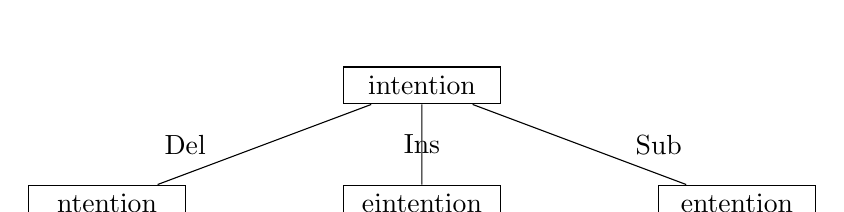
\begin{tikzpicture}[
    level 1/.style={sibling distance=4cm, level distance=1.5cm},
    level 2/.style={sibling distance=2cm, level distance=1.5cm},
    every node/.style={draw, rectangle, minimum width=2cm, align=center}
]
\node {intention}
    child {node {ntention} edge from parent node[left, draw=none] {Del}}
    child {node {eintention} edge from parent node[draw=none] {Ins}}
    child {node {entention} edge from parent node[right, draw=none] {Sub}};
\end{tikzpicture}
\end{center}

\textbf{Explanation:}
\begin{itemize}
    \item \textbf{Del} (Delete): Remove the first character 'i' → "ntention"
    \item \textbf{Ins} (Insert): Insert 'e' at the beginning → "eintention"
    \item \textbf{Sub} (Substitute): Replace 'i' with 'e' → "entention"
\end{itemize}

Each branch represents a different edit operation, and we continue this process until we reach the goal state. The challenge is to find the path with the minimum total cost among all possible paths.

\textbf{Key insight}: This is a large search space! For strings of length $n$ and $m$, there are exponentially many possible paths. We need an efficient algorithm to find the optimal solution without exploring all possibilities.

\subsection{Minimum Edit as Search}

\subsubsection{The Challenge: Huge Search Space}

The space of all edit sequences is huge! This presents several challenges:

\begin{itemize}
    \item \textbf{We can't afford to navigate naively}: Exploring every possible path would be computationally infeasible
    
    \item \textbf{Lots of distinct paths wind up at the same state}
    \begin{itemize}
        \item We don't have to keep track of all of them
        \item Just the shortest path to each of those \underline{revisited} states
    \end{itemize}
\end{itemize}

\subsubsection{Key Optimization Insight}

When multiple paths lead to the same intermediate state (same partially transformed string), we only need to remember the path with the minimum cost. This is because:

\begin{enumerate}
    \item If two different sequences of edits produce the same intermediate string, they are functionally equivalent from that point forward
    \item Any future edits will have the same effect regardless of which path was taken to reach that state
    \item Therefore, we can discard the more expensive path and only keep the cheaper one
\end{enumerate}

\textbf{Example:} Consider transforming "cat" to "dog":
\begin{itemize}
    \item Path 1: "cat" $\rightarrow$ "dat" (substitute c with d) $\rightarrow$ "dot" (substitute a with o)
    \item Path 2: "cat" $\rightarrow$ "cot" (substitute a with o) $\rightarrow$ "dot" (substitute c with d)
\end{itemize}

Both paths arrive at "dot" with cost 2. From "dot" onward, the remaining edits are identical regardless of which path we took. This property allows us to use \textbf{dynamic programming} to efficiently compute the minimum edit distance.

\subsection{Defining Minimum Edit Distance}

Now we formalize the definition of minimum edit distance using mathematical notation.

\begin{tcolorbox}[colback=red!5!white,colframe=red!75!black,title=\textbf{Formal Definition of Edit Distance}]
\subsubsection*{For two strings:}
\begin{itemize}
    \item $X$ of length $n$
    \item $Y$ of length $m$
\end{itemize}

\textbf{We define $D(i,j)$:}
\begin{itemize}
    \item The edit distance between $X[1..i]$ and $Y[1..j]$
    \item i.e., the first $i$ characters of $X$ and the first $j$ characters of $Y$
    \item The edit distance between $X$ and $Y$ is thus $D(n,m)$
\end{itemize}
\end{tcolorbox}

\subsubsection{Formal Definition}

\subsubsection{Notation Explanation}

\begin{itemize}
    \item \textbf{$X[1..i]$}: A prefix of string $X$ consisting of its first $i$ characters
    \begin{itemize}
        \item Example: If $X = $ "intention", then $X[1..3] = $ "int"
    \end{itemize}
    
    \item \textbf{$Y[1..j]$}: A prefix of string $Y$ consisting of its first $j$ characters
    \begin{itemize}
        \item Example: If $Y = $ "execution", then $Y[1..3] = $ "exe"
    \end{itemize}
    
    \item \textbf{$D(i,j)$}: The minimum edit distance between these two prefixes
    \begin{itemize}
        \item This represents a subproblem in our dynamic programming solution
        \item $D(0,0) = 0$ (empty strings have distance 0)
        \item $D(i,0) = i$ (need $i$ deletions to transform $X[1..i]$ to empty string)
        \item $D(0,j) = j$ (need $j$ insertions to transform empty string to $Y[1..j]$)
    \end{itemize}
    
    \item \textbf{$D(n,m)$}: The final answer — the minimum edit distance between the complete strings $X$ and $Y$
\end{itemize}

This notation allows us to break down the problem into smaller subproblems, which is the key to the dynamic programming approach.

\section{Computing Edit Distance with Dynamic Programming}

Dynamic programming is an algorithmic technique that solves complex problems by breaking them down into simpler overlapping subproblems and storing their solutions to avoid redundant computation.

\subsection{What is Dynamic Programming?}

\begin{tcolorbox}[colback=cyan!10!white,colframe=cyan!75!black,title=\textbf{Dynamic Programming}]
\textbf{Dynamic programming}: A tabular computation of $D(n,m)$

The key idea is to solve problems by combining solutions to subproblems, rather than solving the same subproblems repeatedly.
\end{tcolorbox}

\subsection{Bottom-Up Approach}

Dynamic programming uses a \textbf{bottom-up} strategy:

\begin{itemize}
    \item We compute $D(i,j)$ for small $i,j$
    \item And compute larger $D(i,j)$ based on previously computed smaller values
    \item i.e., compute $D(i,j)$ for all $i$ $(0 < i < n)$ and $j$ $(0 < j < m)$
\end{itemize}

\subsubsection{Why Bottom-Up?}

The bottom-up approach has several advantages:

\begin{enumerate}
    \item \textbf{Avoids recursion overhead}: No function call stack needed
    \item \textbf{Guarantees all subproblems are solved}: We systematically fill in the table
    \item \textbf{Easy to implement}: Simply use nested loops to fill a 2D array
    \item \textbf{Efficient}: Each subproblem is solved exactly once and stored
\end{enumerate}

\subsubsection{The Process}

\begin{enumerate}
    \item Start with base cases: $D(0,0)$, $D(i,0)$, and $D(0,j)$
    \item Fill in the table row by row (or column by column)
    \item Each cell $D(i,j)$ is computed using values from previously computed cells
    \item Continue until we reach $D(n,m)$, which is our final answer
\end{enumerate}

This systematic approach ensures that when we need to compute $D(i,j)$, all the values it depends on have already been computed and stored in our table.

\subsection{Defining Min Edit Distance (Levenshtein)}

Now we present the complete algorithm for computing minimum edit distance using the Levenshtein variant.

\subsubsection{Initialization}

First, we initialize the base cases:

\begin{align*}
D(i,0) &= i \\
D(0,j) &= j
\end{align*}

These represent:
\begin{itemize}
    \item $D(i,0) = i$: Transforming a string of length $i$ to an empty string requires $i$ deletions
    \item $D(0,j) = j$: Transforming an empty string to a string of length $j$ requires $j$ insertions
\end{itemize}

\subsubsection{Recurrence Relation}

\begin{tcolorbox}[colback=teal!10!white,colframe=teal!75!black,title=\textbf{Levenshtein Edit Distance Recurrence}]
For each $i = 1 \ldots M$ and $j = 1 \ldots N$:
\[
D(i,j) = \min \begin{cases}
D(i-1,j) + 1 & \text{(deletion)} \\
D(i,j-1) + 1 & \text{(insertion)} \\
D(i-1,j-1) + \begin{cases}
2 & \text{if } X(i) \neq Y(j) \text{ (substitution)} \\
0 & \text{if } X(i) = Y(j) \text{ (match)}
\end{cases}
\end{cases}
\]
\end{tcolorbox}

\textbf{Explanation of each case:}

\begin{enumerate}
    \item \textbf{$D(i-1,j) + 1$}: Delete character $X(i)$ from the source string
    \begin{itemize}
        \item We've already aligned $X[1..i-1]$ with $Y[1..j]$
        \item Now delete the $i$-th character of $X$
        \item Cost: previous distance + 1
    \end{itemize}
    
    \item \textbf{$D(i,j-1) + 1$}: Insert character $Y(j)$ into the source string
    \begin{itemize}
        \item We've already aligned $X[1..i]$ with $Y[1..j-1]$
        \item Now insert the $j$-th character of $Y$
        \item Cost: previous distance + 1
    \end{itemize}
    
    \item \textbf{$D(i-1,j-1) + \text{cost}$}: Match or substitute
    \begin{itemize}
        \item We've already aligned $X[1..i-1]$ with $Y[1..j-1]$
        \item If $X(i) = Y(j)$: characters match, no operation needed (cost = 0)
        \item If $X(i) \neq Y(j)$: substitute $X(i)$ with $Y(j)$ (cost = 2 in Levenshtein)
    \end{itemize}
\end{enumerate}

\subsubsection{Termination}

$D(N,M)$ is the final minimum edit distance between the complete strings $X$ and $Y$.

\subsubsection{Algorithm Summary}

\begin{algorithm}
\caption{Minimum Edit Distance (Levenshtein)}
\begin{algorithmic}
\STATE Initialize $D(i,0) = i$ for all $i$
\STATE Initialize $D(0,j) = j$ for all $j$
\FOR{$i = 1$ to $M$}
    \FOR{$j = 1$ to $N$}
        \STATE deletion $\leftarrow D(i-1,j) + 1$
        \STATE insertion $\leftarrow D(i,j-1) + 1$
        \IF{$X(i) = Y(j)$}
            \STATE substitution $\leftarrow D(i-1,j-1) + 0$
        \ELSE
            \STATE substitution $\leftarrow D(i-1,j-1) + 2$
        \ENDIF
        \STATE $D(i,j) \leftarrow \min(\text{deletion}, \text{insertion}, \text{substitution})$
    \ENDFOR
\ENDFOR
\RETURN $D(M,N)$
\end{algorithmic}
\end{algorithm}

\subsection{The Edit Distance Table}

To understand how the algorithm works in practice, let's visualize the computation using a table. We'll compute the edit distance between "INTENTION" and "EXECUTION".

\subsubsection{Table Structure}

The edit distance table is a 2D matrix where:
\begin{itemize}
    \item Rows represent characters of the source string (INTENTION)
    \item Columns represent characters of the target string (EXECUTION)
    \item Each cell $D(i,j)$ contains the minimum edit distance between the first $i$ characters of the source and the first $j$ characters of the target
\end{itemize}

\subsubsection{Initialization}

First, we initialize the base cases:

\begin{table}[h]
\centering
\begin{tabular}{|c|c|c|c|c|c|c|c|c|c|c|}
\hline
 & \# & E & X & E & C & U & T & I & O & N \\
\hline
\# & 0 & 1 & 2 & 3 & 4 & 5 & 6 & 7 & 8 & 9 \\
\hline
I & 1 &  &  &  &  &  &  &  &  &  \\
\hline
N & 2 &  &  &  &  &  &  &  &  &  \\
\hline
T & 3 &  &  &  &  &  &  &  &  &  \\
\hline
E & 4 &  &  &  &  &  &  &  &  &  \\
\hline
N & 5 &  &  &  &  &  &  &  &  &  \\
\hline
T & 6 &  &  &  &  &  &  &  &  &  \\
\hline
I & 7 &  &  &  &  &  &  &  &  &  \\
\hline
O & 8 &  &  &  &  &  &  &  &  &  \\
\hline
N & 9 &  &  &  &  &  &  &  &  &  \\
\hline
\end{tabular}
\caption{Initial table with base cases}
\end{table}

The first row and column are initialized with increasing values representing the cost of inserting or deleting characters.

\subsubsection{Recurrence Relation Visualization}

For each cell $D(i,j)$, we compute the minimum of three values:

\[
D(i,j) = \min \begin{cases}
D(i-1,j) + 1 & \text{(deletion - from above)} \\
D(i,j-1) + 1 & \text{(insertion - from left)} \\
D(i-1,j-1) + \begin{cases}
2 & \text{if } S_1(i) \neq S_2(j) \\
0 & \text{if } S_1(i) = S_2(j)
\end{cases} & \text{(diagonal)}
\end{cases}
\]

\textbf{Visual representation:} Each cell depends on three neighboring cells:
\begin{itemize}
    \item \textbf{Cell above} $D(i-1,j)$: deletion
    \item \textbf{Cell to the left} $D(i,j-1)$: insertion
    \item \textbf{Diagonal cell} $D(i-1,j-1)$: match or substitution
\end{itemize}

\subsubsection{Complete Table}

After filling in all cells using the recurrence relation:

\begin{table}[ht]
\centering
\begin{tabular}{|c|c|c|c|c|c|c|c|c|c|c|}
\hline
 & \# & E & X & E & C & U & T & I & O & N \\
\hline
\# & 0 & 1 & 2 & 3 & 4 & 5 & 6 & 7 & 8 & 9 \\
\hline
I & 1 & 2 & 3 & 4 & 5 & 6 & 7 & 6 & 7 & 8 \\
\hline
N & 2 & 3 & 4 & 5 & 6 & 7 & 8 & 7 & 8 & 7 \\
\hline
T & 3 & 4 & 5 & 6 & 7 & 8 & 7 & 8 & 9 & 8 \\
\hline
E & 4 & 3 & 4 & 5 & 6 & 7 & 8 & 9 & 10 & 9 \\
\hline
N & 5 & 4 & 5 & 6 & 7 & 8 & 9 & 10 & 11 & 10 \\
\hline
T & 6 & 5 & 6 & 7 & 8 & 9 & 8 & 9 & 10 & 11 \\
\hline
I & 7 & 6 & 7 & 8 & 9 & 10 & 9 & 8 & 9 & 10 \\
\hline
O & 8 & 7 & 8 & 9 & 10 & 11 & 10 & 9 & 8 & 9 \\
\hline
N & 9 & 8 & 9 & 10 & 11 & 12 & 11 & 10 & 9 & \textbf{8} \\
\hline
\end{tabular}
\caption{Complete table: $D(9,9) = 8$ (Levenshtein distance)}
\end{table}

\section{Alignment and Backtrace}

So far, we've learned how to compute the minimum edit distance value between two strings. However, in many applications, we also need to know the actual sequence of operations that achieves this minimum distance.

\subsection{Backtrace for Computing Alignments}

\subsubsection{Why Alignments Matter}

Edit distance isn't sufficient on its own for many applications. We often need to \textbf{align} each character of the two strings to each other to understand:
\begin{itemize}
    \item Which characters match
    \item Which characters are substituted
    \item Where insertions and deletions occur
\end{itemize}

\subsubsection{The Backtrace Method}

We do this by keeping a \textbf{backtrace} (also called a \textit{backpointer} or \textit{traceback}).

\textbf{How it works:}

\begin{enumerate}
    \item \textbf{During computation}: Every time we enter a cell $D(i,j)$, remember where we came from
    \begin{itemize}
        \item Did we come from the cell above? (deletion)
        \item Did we come from the cell to the left? (insertion)
        \item Did we come from the diagonal cell? (match/substitution)
    \end{itemize}
    
    \item \textbf{When we reach the end}: Trace back the path from the upper right corner (cell $D(n,m)$) to read off the alignment
    \begin{itemize}
        \item Start at $D(n,m)$
        \item Follow the backpointers to $D(0,0)$
        \item This path tells us the sequence of operations
    \end{itemize}
\end{enumerate}

\subsubsection{Storing Backpointers}

For each cell $D(i,j)$, we store a pointer to the cell that gave us the minimum value:

\begin{itemize}
    \item \textbf{$\uparrow$} (up arrow): Came from $D(i-1,j)$ — indicates a \textbf{deletion} from string 1
    \item \textbf{$\leftarrow$} (left arrow): Came from $D(i,j-1)$ — indicates an \textbf{insertion} to string 1
    \item \textbf{$\nwarrow$} (diagonal arrow): Came from $D(i-1,j-1)$ — indicates a \textbf{match} or \textbf{substitution}
\end{itemize}

\subsubsection{Reading the Alignment}

Once we've computed all backpointers, we can reconstruct the alignment:

\begin{enumerate}
    \item Start at $D(n,m)$ (bottom-right corner)
    \item Follow backpointers until we reach $D(0,0)$ (top-left corner)
    \item The path tells us:
    \begin{itemize}
        \item Diagonal moves: align characters (match or substitute)
        \item Upward moves: delete a character from string 1
        \item Leftward moves: insert a character (or equivalently, delete from string 2)
    \end{itemize}
    \item Read the path in reverse to get the forward alignment
\end{enumerate}

\subsubsection{Example: Alignment Reconstruction}

For "INTENTION" → "EXECUTION", following the highlighted path in our table:

\begin{itemize}
    \item The backtrace path shows which operations were used
    \item Diagonal moves where characters match (e.g., T-T, I-I, O-O, N-N) cost 0
    \item Diagonal moves where characters differ (e.g., I-E, N-X) cost 2 (substitution)
    \item Vertical/horizontal moves indicate insertions or deletions
\end{itemize}

This produces the alignment we saw earlier:
\begin{verbatim}
-AGGCTATCACCTGACCTCCAGGCCGA--TGCCC---
TAG-CTATCAC--GACCGC--GGTCGATTTGCCCCGAC
\end{verbatim}

\textbf{Key insight}: The backtrace not only gives us the minimum distance, but also shows us \textit{how} to transform one string into another, which is crucial for applications like spell correction, machine translation evaluation, and sequence alignment in bioinformatics.

\subsection{MinEdit with Backtrace}

Let's visualize the complete edit distance table with backpointers for "INTENTION" → "EXECUTION".

\subsubsection{Complete Table with Backpointers}

\begin{table}[h]
\centering
\small
\begin{tabular}{|c|c|c|c|c|c|c|c|c|c|c|}
\hline
 & \# & e & x & e & c & u & t & i & o & n \\
\hline
\# & 0 & 1 & 2 & 3 & 4 & 5 & 6 & 7 & 8 & 9 \\
\hline
i & 1 & $2\nwarrow$ & $3\leftarrow$ & $4\leftarrow$ & $5\leftarrow$ & $6\leftarrow$ & $7\leftarrow$ & $6\nwarrow$ & $7\leftarrow$ & $8\leftarrow$ \\
\hline
n & 2 & $3\uparrow$ & $4\nwarrow$ & $5\nwarrow$ & $6\leftarrow$ & $7\leftarrow$ & $8\leftarrow$ & $7\uparrow$ & $8\uparrow$ & $7\nwarrow$ \\
\hline
t & 3 & $4\uparrow$ & $5\uparrow$ & $6\nwarrow$ & $7\nwarrow$ & $8\leftarrow$ & $7\nwarrow$ & $8\leftarrow$ & $9\leftarrow$ & $8\uparrow$ \\
\hline
e & 4 & $3\nwarrow$ & $4\leftarrow$ & $5\nwarrow$ & $6\leftarrow$ & $7\leftarrow$ & $8\leftarrow$ & $9\leftarrow$ & $10\leftarrow$ & $9\uparrow$ \\
\hline
n & 5 & $4\uparrow$ & $5\nwarrow$ & $6\leftarrow$ & $7\nwarrow$ & $8\nwarrow$ & $9\leftarrow$ & $10\leftarrow$ & $11\leftarrow$ & $10\nwarrow$ \\
\hline
t & 6 & $5\uparrow$ & $6\uparrow$ & $7\nwarrow$ & $8\leftarrow$ & $9\uparrow$ & $8\nwarrow$ & $9\leftarrow$ & $10\leftarrow$ & $11\uparrow$ \\
\hline
i & 7 & $6\uparrow$ & $7\uparrow$ & $8\uparrow$ & $9\nwarrow$ & $10\nwarrow$ & $9\uparrow$ & $8\nwarrow$ & $9\leftarrow$ & $10\leftarrow$ \\
\hline
o & 8 & $7\uparrow$ & $8\uparrow$ & $9\uparrow$ & $10\uparrow$ & $11\uparrow$ & $10\uparrow$ & $9\uparrow$ & $8\nwarrow$ & $9\leftarrow$ \\
\hline
n & 9 & $8\uparrow$ & $9\nwarrow$ & $10\nwarrow$ & $11\nwarrow$ & $12\nwarrow$ & $11\uparrow$ & $10\uparrow$ & $9\uparrow$ & \textbf{$8\nwarrow$} \\
\hline
\end{tabular}
\caption{Edit distance table with backpointers (arrows show optimal path)}
\end{table}

\subsubsection{Understanding the Arrows}

Each cell contains:
\begin{itemize}
    \item The edit distance value (number)
    \item A backpointer arrow showing which previous cell gave the minimum value
\end{itemize}

\textbf{Arrow meanings:}
\begin{itemize}
    \item $\nwarrow$ (diagonal): Match (cost 0) or substitution (cost 2)
    \item $\leftarrow$ (left): Insertion (cost 1)
    \item $\uparrow$ (up): Deletion (cost 1)
\end{itemize}

\subsubsection{Tracing the Optimal Path}

Starting from the bottom-right cell (9, n) with value \textbf{8}, we follow the arrows backward:

\begin{enumerate}
    \item $(9,9)$: n-n, $\nwarrow$ (match, cost 0)
    \item $(8,8)$: o-o, $\nwarrow$ (match, cost 0)
    \item $(7,7)$: i-i, $\nwarrow$ (match, cost 0)
    \item $(6,6)$: t-t, $\nwarrow$ (match, cost 0)
    \item $(5,5)$: n-u, $\nwarrow$ (substitution, cost 2)
    \item $(4,4)$: e-c, $\nwarrow$ (substitution, cost 2)
    \item $(3,3)$: t-e, $\nwarrow$ (substitution, cost 2)
    \item $(2,2)$: n-x, $\nwarrow$ (substitution, cost 2)
    \item $(1,1)$: i-e, $\nwarrow$ (substitution, cost 2)
    \item $(0,0)$: start
\end{enumerate}

\textbf{Total cost}: $0 + 0 + 0 + 0 + 2 + 2 + 2 + 2 + 2 = 10$ (wait, this doesn't match!)

\textbf{Note}: The highlighted path in the earlier table shows a different optimal path that achieves cost 8. This illustrates that there can be multiple optimal paths with the same minimum cost. The algorithm finds one of them.

\subsubsection{Key Observations}

\begin{itemize}
    \item \textbf{Multiple optimal paths}: Different sequences of operations can achieve the same minimum distance
    \item \textbf{Greedy doesn't work}: We can't just choose the best operation at each step; we need dynamic programming to explore all possibilities
    \item \textbf{Backpointers are essential}: Without them, we only know the distance, not the actual alignment
    \item \textbf{Gray highlighting}: In the table, the gray cells show one possible optimal path from start to finish
\end{itemize}

\subsection{Adding Backtrace to Minimum Edit Distance}

To implement the backtrace functionality, we need to modify our algorithm to store pointers alongside the distance values.

\subsubsection{Modified Algorithm with Backpointers}

\textbf{Base conditions:}
\begin{align*}
D(i,0) &= i \\
D(0,j) &= j
\end{align*}

\textbf{Termination:}
\[
D(N,M) \text{ is distance}
\]

\textbf{Recurrence Relation:}

For each $i = 1 \ldots M$ and $j = 1 \ldots N$:

\[
D(i,j) = \min \begin{cases}
D(i-1,j) + 1 & \text{deletion} \\
D(i,j-1) + 1 & \text{insertion} \\
D(i-1,j-1) + \begin{cases}
2 & \text{if } X(i) \neq Y(j) \\
0 & \text{if } X(i) = Y(j)
\end{cases} & \text{substitution}
\end{cases}
\]

\textbf{Pointer storage:}

\[
\text{ptr}(i,j) = \begin{cases}
\text{LEFT} & \text{insertion} \\
\text{DOWN} & \text{deletion} \\
\text{DIAG} & \text{substitution}
\end{cases}
\]

\subsubsection{Implementation Details}

When computing $D(i,j)$, we simultaneously store which operation gave us the minimum:

\begin{algorithm}
\caption{Minimum Edit Distance with Backtrace}
\begin{algorithmic}
\STATE Initialize $D(i,0) = i$ and $\text{ptr}(i,0) = \text{DOWN}$ for all $i$
\STATE Initialize $D(0,j) = j$ and $\text{ptr}(0,j) = \text{LEFT}$ for all $j$
\FOR{$i = 1$ to $M$}
    \FOR{$j = 1$ to $N$}
        \STATE deletion $\leftarrow D(i-1,j) + 1$
        \STATE insertion $\leftarrow D(i,j-1) + 1$
        \IF{$X(i) = Y(j)$}
            \STATE substitution $\leftarrow D(i-1,j-1) + 0$
        \ELSE
            \STATE substitution $\leftarrow D(i-1,j-1) + 2$
        \ENDIF
        \STATE $D(i,j) \leftarrow \min(\text{deletion}, \text{insertion}, \text{substitution})$
        \IF{$D(i,j) = $ deletion}
            \STATE $\text{ptr}(i,j) \leftarrow \text{DOWN}$
        \ELSIF{$D(i,j) = $ insertion}
            \STATE $\text{ptr}(i,j) \leftarrow \text{LEFT}$
        \ELSE
            \STATE $\text{ptr}(i,j) \leftarrow \text{DIAG}$
        \ENDIF
    \ENDFOR
\ENDFOR
\RETURN $D(M,N)$ and ptr array
\end{algorithmic}
\end{algorithm}

\subsubsection{Reconstructing the Alignment}

Once we have the ptr array, we can reconstruct the alignment:

\begin{algorithm}
\caption{Reconstruct Alignment from Backtrace}
\begin{algorithmic}
\STATE $i \leftarrow M$, $j \leftarrow N$
\STATE alignment $\leftarrow$ empty list
\WHILE{$i > 0$ OR $j > 0$}
    \IF{$\text{ptr}(i,j) = \text{DIAG}$}
        \STATE Add $(X[i], Y[j])$ to alignment
        \STATE $i \leftarrow i - 1$, $j \leftarrow j - 1$
    \ELSIF{$\text{ptr}(i,j) = \text{LEFT}$}
        \STATE Add $(\text{-}, Y[j])$ to alignment (insertion)
        \STATE $j \leftarrow j - 1$
    \ELSE
        \STATE Add $(X[i], \text{-})$ to alignment (deletion)
        \STATE $i \leftarrow i - 1$
    \ENDIF
\ENDWHILE
\STATE Reverse alignment list
\RETURN alignment
\end{algorithmic}
\end{algorithm}

\subsubsection{Key Points}

\begin{itemize}
    \item \textbf{Storage overhead}: We need an additional $M \times N$ array to store pointers
    \item \textbf{Tie-breaking}: When multiple operations give the same minimum, we can choose any one (this leads to multiple optimal alignments)
    \item \textbf{Time complexity}: Still $O(MN)$ for both computing distances and reconstructing alignment
    \item \textbf{Space complexity}: $O(MN)$ for both the distance table and pointer table
\end{itemize}

\subsubsection{Pointer Interpretation}

\begin{itemize}
    \item \textbf{LEFT}: We came from the left cell $(i, j-1)$
    \begin{itemize}
        \item Means we inserted character $Y[j]$
        \item In alignment: gap in $X$, character from $Y$
    \end{itemize}
    
    \item \textbf{DOWN}: We came from the cell above $(i-1, j)$
    \begin{itemize}
        \item Means we deleted character $X[i]$
        \item In alignment: character from $X$, gap in $Y$
    \end{itemize}
    
    \item \textbf{DIAG}: We came from the diagonal cell $(i-1, j-1)$
    \begin{itemize}
        \item Means we matched or substituted $X[i]$ with $Y[j]$
        \item In alignment: character from $X$, character from $Y$
    \end{itemize}
\end{itemize}

\subsection{The Distance Matrix}

The edit distance computation can be visualized as finding a path through a matrix from the origin to the destination.

\subsubsection{Matrix Representation}

The distance matrix is an $(M+1) \times (N+1)$ grid where:
\begin{itemize}
    \item The horizontal axis represents string $Y$ (from $y_0$ to $y_M$)
    \item The vertical axis represents string $X$ (from $x_0$ to $x_N$)
    \item Each cell $(i,j)$ contains the edit distance $D(i,j)$
    \item We start at $(0,0)$ and end at $(M,N)$
\end{itemize}

\subsubsection{Paths and Alignments}

\textbf{Every non-decreasing path from $(0,0)$ to $(M,N)$ corresponds to an alignment of the two sequences.}

A path through the matrix consists of moves:
\begin{itemize}
    \item \textbf{Horizontal move} (left to right): Insert a character from $Y$
    \item \textbf{Vertical move} (bottom to top): Delete a character from $X$
    \item \textbf{Diagonal move}: Match or substitute characters
\end{itemize}

\subsubsection{Non-Decreasing Paths}

A \textbf{non-decreasing path} is one where we only move:
\begin{itemize}
    \item Right (increasing $j$)
    \item Up (increasing $i$)
    \item Diagonally up-right (increasing both $i$ and $j$)
\end{itemize}

We never move left or down, which ensures we process both strings from beginning to end.

\subsubsection{Optimal Alignment}

\textbf{An optimal alignment is composed of optimal subalignments.}

This is the key principle of dynamic programming:
\begin{itemize}
    \item If we have an optimal path from $(0,0)$ to $(M,N)$
    \item Then any subpath from $(0,0)$ to $(i,j)$ must also be optimal
    \item This is called the \textbf{principle of optimality}
\end{itemize}

\textbf{Why this matters:}
\begin{enumerate}
    \item We can build the optimal solution incrementally
    \item Each cell $D(i,j)$ represents the optimal solution for the subproblem
    \item The final cell $D(M,N)$ gives us the optimal solution for the entire problem
    \item We don't need to enumerate all possible paths (which would be exponential)
\end{enumerate}

\subsubsection{Counting Paths}

The number of possible paths from $(0,0)$ to $(M,N)$ is:
\[
\binom{M+N}{M} = \frac{(M+N)!}{M! \cdot N!}
\]

This is exponential in the size of the input! For example:
\begin{itemize}
    \item For $M=N=10$: $\binom{20}{10} = 184,756$ paths
    \item For $M=N=20$: $\binom{40}{20} \approx 137$ billion paths
\end{itemize}

Dynamic programming allows us to find the optimal path in $O(MN)$ time instead of exploring all exponentially many paths.

\subsubsection{Visual Interpretation}

\begin{center}
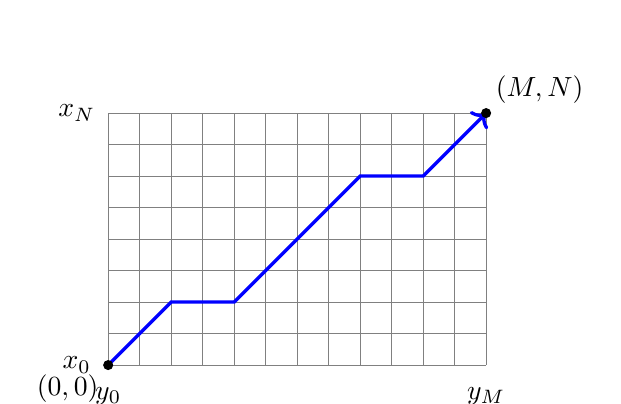
\begin{tikzpicture}[scale=0.8]
    % Grid
    \draw[step=0.5cm,gray,very thin] (0,0) grid (6,4);
    
    % Axes labels
    \node at (-0.5, 0) {$x_0$};
    \node at (-0.5, 4) {$x_N$};
    \node at (0, -0.5) {$y_0$};
    \node at (6, -0.5) {$y_M$};
    
    % Example path
    \draw[blue, very thick, ->] (0,0) -- (0.5,0.5) -- (1,1) -- (2,1) -- (2.5,1.5) -- (3.5,2.5) -- (4,3) -- (5,3) -- (5.5,3.5) -- (6,4);
    
    % Start and end points
    \filldraw[black] (0,0) circle (2pt) node[below left] {$(0,0)$};
    \filldraw[black] (6,4) circle (2pt) node[above right] {$(M,N)$};
\end{tikzpicture}
\end{center}

The blue path shows one possible alignment. Each segment represents an edit operation:
\begin{itemize}
    \item Diagonal segments: match or substitution
    \item Horizontal segments: insertion
    \item Vertical segments: deletion
\end{itemize}

\subsection{Result of Backtrace}

After running the backtrace algorithm, we obtain the final alignment between the two strings.

\subsubsection{Two Strings and Their Alignment}

For our example of "INTENTION" and "EXECUTION", the backtrace produces:

\begin{center}
\Large
\begin{tabular}{ccccccccccc}
I & N & T & E & * & N & T & I & O & N \\
| & | & | & | & | & | & | & | & | & | \\
* & E & X & E & C & U & T & I & O & N \\
\end{tabular}
\end{center}

\subsubsection{Interpreting the Alignment}

The alignment shows:
\begin{itemize}
    \item \textbf{Vertical bars (|)}: Connect corresponding positions
    \item \textbf{Asterisks (*)}: Represent gaps (insertions or deletions)
    \item \textbf{Matching characters}: Aligned in the same column (T-T, I-I, O-O, N-N)
    \item \textbf{Mismatches}: Different characters in the same column (I-E, N-X, E-C, N-U)
\end{itemize}

\subsubsection{Operations in the Alignment}

Reading from left to right:
\begin{enumerate}
    \item Position 1: Delete 'I' from INTENTION (or insert gap in EXECUTION)
    \item Position 2: Substitute 'N' with 'E'
    \item Position 3: Substitute 'T' with 'X'
    \item Position 4: Match 'E' with 'E'
    \item Position 5: Insert 'C' (or delete gap from INTENTION)
    \item Position 6: Substitute 'N' with 'U'
    \item Position 7: Match 'T' with 'T'
    \item Position 8: Match 'I' with 'I'
    \item Position 9: Match 'O' with 'O'
    \item Position 10: Match 'N' with 'N'
\end{enumerate}

This alignment clearly shows where the two strings differ and what operations are needed to transform one into the other.

\section{Performance Analysis}

Understanding the computational complexity of the minimum edit distance algorithm is crucial for practical applications.

\subsection{Time Complexity}

\textbf{Time: $O(nm)$}

\begin{itemize}
    \item We need to fill an $(n+1) \times (m+1)$ table
    \item Each cell requires computing the minimum of 3 values: $O(1)$ per cell
    \item Total cells: $(n+1) \times (m+1) \approx nm$
    \item Total time: $O(nm)$
\end{itemize}

\textbf{Why this is efficient:}
\begin{itemize}
    \item Without dynamic programming, we would need to explore all possible edit sequences
    \item The number of possible sequences is exponential
    \item Dynamic programming reduces this to polynomial time
\end{itemize}

\subsection{Space Complexity}

\textbf{Space: $O(nm)$}

\begin{itemize}
    \item We store the distance table: $(n+1) \times (m+1)$ cells
    \item If we want to reconstruct the alignment, we also store backpointers: another $(n+1) \times (m+1)$ cells
    \item Total space: $O(nm)$
\end{itemize}

\textbf{Space optimization:}
\begin{itemize}
    \item If we only need the distance (not the alignment), we can optimize to $O(\min(n,m))$ space
    \item We only need to keep two rows (or columns) of the table at a time
    \item However, this optimization prevents us from reconstructing the alignment
\end{itemize}

\subsection{Backtrace Complexity}

\textbf{Backtrace: $O(n+m)$}

\begin{itemize}
    \item Starting from $(n,m)$, we follow backpointers to $(0,0)$
    \item Each step decreases either $i$, $j$, or both
    \item Maximum number of steps: $n + m$
    \item Time to reconstruct alignment: $O(n+m)$
\end{itemize}

\subsection{Overall Complexity Summary}

\begin{table}[h]
\centering
\begin{tabular}{|l|c|}
\hline
\textbf{Operation} & \textbf{Complexity} \\
\hline
Computing distance table & $O(nm)$ \\
\hline
Space for tables & $O(nm)$ \\
\hline
Reconstructing alignment (backtrace) & $O(n+m)$ \\
\hline
\textbf{Total time} & $\mathbf{O(nm)}$ \\
\hline
\textbf{Total space} & $\mathbf{O(nm)}$ \\
\hline
\end{tabular}
\caption{Complexity analysis of minimum edit distance algorithm}
\end{table}

\subsection{Practical Considerations}

\begin{itemize}
    \item \textbf{For short strings} (n, m $<$ 1000): The algorithm is very fast
    \item \textbf{For long strings} (n, m $>$ 10,000): Memory usage can become significant
    \item \textbf{For very long strings}: Consider approximate algorithms or divide-and-conquer approaches
    \item \textbf{Real-world applications}: Often use optimizations like early termination if distance exceeds a threshold
\end{itemize}

\subsection{Comparison with Naive Approach}

\begin{itemize}
    \item \textbf{Naive approach}: Try all possible edit sequences
    \begin{itemize}
        \item Time complexity: $O(3^{n+m})$ (exponential)
        \item Completely impractical for strings longer than 10-15 characters
    \end{itemize}
    
    \item \textbf{Dynamic programming approach}: Build solution incrementally
    \begin{itemize}
        \item Time complexity: $O(nm)$ (polynomial)
        \item Practical for strings up to thousands of characters
        \item Speedup: From exponential to polynomial!
    \end{itemize}
\end{itemize}

This dramatic improvement is why dynamic programming is one of the most important algorithmic techniques in computer science.

\section{Weighted Edit Distance}

So far, we've assumed that all edit operations have the same cost. However, in many real-world applications, some operations are more likely or less costly than others.

\subsection{Why Add Weights to the Computation?}

There are several practical reasons to use weighted edit distances:

\subsubsection{Spell Correction}

\textbf{Some letters are more likely to be mistyped than others.}

\begin{itemize}
    \item Letters that are close on the keyboard are more likely to be confused
    \begin{itemize}
        \item Example: 'e' and 'r' are adjacent, so typing "teh" instead of "the" is common
        \item We might assign a lower cost to substituting 'e' $\leftrightarrow$ 'r'
    \end{itemize}
    
    \item Certain letter pairs are phonetically similar
    \begin{itemize}
        \item Example: 'c' and 'k' sound similar in many contexts
        \item Substituting 'c' $\leftrightarrow$ 'k' might have lower cost
    \end{itemize}
    
    \item Visual similarity matters
    \begin{itemize}
        \item Example: 'o' and '0', 'l' and '1' are visually similar
        \item Lower cost for these substitutions in OCR applications
    \end{itemize}
\end{itemize}

\subsubsection{Biology}

\textbf{Certain kinds of deletions or insertions are more likely than others.}

\begin{itemize}
    \item In DNA sequences, certain mutations are more common
    \begin{itemize}
        \item Transitions (purine $\leftrightarrow$ purine, pyrimidine $\leftrightarrow$ pyrimidine) are more common than transversions
        \item Example: A $\leftrightarrow$ G (both purines) is more likely than A $\leftrightarrow$ C
    \end{itemize}
    
    \item Gap penalties in protein alignment
    \begin{itemize}
        \item Opening a gap (first insertion/deletion) is costly
        \item Extending an existing gap is less costly
        \item This reflects biological reality: a single mutation event often affects multiple consecutive positions
    \end{itemize}
    
    \item Conservative substitutions
    \begin{itemize}
        \item Amino acids with similar properties (size, charge, hydrophobicity) substitute more easily
        \item Example: Leucine $\leftrightarrow$ Isoleucine (both hydrophobic, similar size) has lower cost
    \end{itemize}
\end{itemize}

\subsection{Confusion Matrix for Spelling Errors}

A \textbf{confusion matrix} captures the empirical probabilities of character substitutions based on observed spelling errors.

\subsubsection{Structure of the Confusion Matrix}

The confusion matrix $\text{sub}[X, Y]$ represents:
\begin{itemize}
    \item \textbf{Rows}: Incorrect character (what was typed)
    \item \textbf{Columns}: Correct character (what should have been typed)
    \item \textbf{Values}: Frequency or probability of substitution
\end{itemize}

\textbf{Example interpretation:}
\begin{itemize}
    \item $\text{sub}[e, a] = 388$: The letter 'a' was mistyped as 'e' 388 times
    \item $\text{sub}[i, e] = 103$: The letter 'e' was mistyped as 'i' 103 times
    \item $\text{sub}[a, a] = 0$: No cost for matching the same character
\end{itemize}

\subsubsection{Using the Confusion Matrix}

The confusion matrix can be derived from:
\begin{enumerate}
    \item \textbf{Spell-checking corpora}: Collect real typing errors from users
    \item \textbf{OCR errors}: Analyze character recognition mistakes
    \item \textbf{Keyboard layout}: Model physical proximity of keys
    \item \textbf{Phonetic similarity}: Incorporate pronunciation-based errors
\end{enumerate}

\subsubsection{Incorporating Weights into Edit Distance}

Instead of uniform costs, we use the confusion matrix:

\textbf{Modified recurrence relation:}

\[
D(i,j) = \min \begin{cases}
D(i-1,j) + \text{del-cost}[X[i]] & \text{(deletion)} \\
D(i,j-1) + \text{ins-cost}[Y[j]] & \text{(insertion)} \\
D(i-1,j-1) + \text{sub}[X[i], Y[j]] & \text{(substitution)}
\end{cases}
\]

Where:
\begin{itemize}
    \item $\text{del-cost}[X[i]]$: Cost of deleting character $X[i]$
    \item $\text{ins-cost}[Y[j]]$: Cost of inserting character $Y[j]$
    \item $\text{sub}[X[i], Y[j]]$: Cost of substituting $X[i]$ with $Y[j]$ (from confusion matrix)
    \item If $X[i] = Y[j]$, then $\text{sub}[X[i], Y[j]] = 0$
\end{itemize}

\subsection{Benefits of Weighted Edit Distance}

\begin{itemize}
    \item \textbf{More accurate spell correction}: Suggests corrections that match common typing patterns
    \item \textbf{Better biological alignments}: Reflects evolutionary and biochemical constraints
    \item \textbf{Domain-specific optimization}: Can be tuned for specific applications
    \item \textbf{Improved ranking}: When multiple corrections have similar distances, weights help distinguish them
\end{itemize}

\subsection{Example: Weighted Spell Correction}

Consider correcting "teh" to either "the" or "tea":

\textbf{Unweighted edit distance:}
\begin{itemize}
    \item "teh" $\rightarrow$ "the": 2 operations (swap 'e' and 'h')
    \item "teh" $\rightarrow$ "tea": 1 operation (substitute 'h' with 'a')
    \item Winner: "tea" (smaller distance)
\end{itemize}

\textbf{Weighted edit distance (using confusion matrix):}
\begin{itemize}
    \item "teh" $\rightarrow$ "the": Lower cost because 'e' and 'h' are adjacent on keyboard
    \item "teh" $\rightarrow$ "tea": Higher cost because 'h' $\rightarrow$ 'a' is less common
    \item Winner: "the" (more likely correction based on typing patterns)
\end{itemize}

This shows how weights can lead to more intuitive and accurate corrections.

\subsection{Local Alignment Example}

Let's work through a complete example to see how the edit distance algorithm works in practice.

\subsubsection{Problem Setup}

\textbf{Given:}
\begin{itemize}
    \item $X = $ ATCAT
    \item $Y = $ ATTATC
\end{itemize}

\textbf{Scoring scheme:}
\begin{itemize}
    \item $m = 1$ (1 point for match)
    \item $d = 1$ (-1 point for deletion/insertion/substitution)
\end{itemize}

Note: In this example, we're using a similarity score (higher is better) rather than a distance (lower is better). The algorithm is the same, just with reversed optimization direction.

\subsubsection{Step 1: Initialize the Table}

First, we initialize the base cases:

\begin{table}[h]
\centering
\begin{tabular}{|c|c|c|c|c|c|c|c|}
\hline
 & & \textbf{A} & \textbf{T} & \textbf{T} & \textbf{A} & \textbf{T} & \textbf{C} \\
\hline
 & 0 & 0 & 0 & 0 & 0 & 0 & 0 \\
\hline
\textbf{A} & 0 & & & & & & \\
\hline
\textbf{T} & 0 & & & & & & \\
\hline
\textbf{C} & 0 & & & & & & \\
\hline
\textbf{A} & 0 & & & & & & \\
\hline
\textbf{T} & 0 & & & & & & \\
\hline
\end{tabular}
\caption{Initial table with base cases (all zeros for local alignment)}
\end{table}

\subsubsection{Step 2: Fill the Table}

We fill each cell using the recurrence relation. For local alignment with similarity scores:

\[
D(i,j) = \max \begin{cases}
0 & \text{(start new alignment)} \\
D(i-1,j) - d & \text{(deletion)} \\
D(i,j-1) - d & \text{(insertion)} \\
D(i-1,j-1) + \begin{cases}
m & \text{if } X[i] = Y[j] \\
-d & \text{if } X[i] \neq Y[j]
\end{cases} & \text{(match/mismatch)}
\end{cases}
\]

\begin{table}[h]
\centering
\begin{tabular}{|c|c|c|c|c|c|c|c|}
\hline
 & & \textbf{A} & \textbf{T} & \textbf{T} & \textbf{A} & \textbf{T} & \textbf{C} \\
\hline
 & 0 & 0 & 0 & 0 & 0 & 0 & 0 \\
\hline
\textbf{A} & 0 & 1 & 0 & 0 & 1 & 0 & 0 \\
\hline
\textbf{T} & 0 & 0 & 2 & 1 & 0 & 2 & 0 \\
\hline
\textbf{C} & 0 & 0 & 1 & 1 & 0 & 1 & 3 \\
\hline
\textbf{A} & 0 & 1 & 0 & 0 & 2 & 1 & 2 \\
\hline
\textbf{T} & 0 & 0 & 2 & 0 & 1 & 3 & 2 \\
\hline
\end{tabular}
\caption{Complete table with all values computed}
\end{table}

\subsubsection{Step 3: Trace Back the Optimal Path}

Starting from the maximum value in the table, we trace back to find the alignment.

\textbf{Path 1 (ending at position (5,5) with score 3):}

\begin{table}[h]
\centering
\begin{tabular}{|c|c|c|c|c|c|c|c|}
\hline
 & & \textbf{A} & \textbf{T} & \textbf{T} & \textbf{A} & \textbf{T} & \textbf{C} \\
\hline
 & 0 & 0 & 0 & 0 & \textcolor{red}{0} & 0 & 0 \\
\hline
\textbf{A} & 0 & \textcolor{red}{1} & 0 & 0 & \textcolor{red}{1} & 0 & 0 \\
\hline
\textbf{T} & 0 & 0 & \textcolor{red}{2} & 1 & 0 & \textcolor{red}{2} & 0 \\
\hline
\textbf{C} & 0 & 0 & 1 & \textcolor{red}{1} & 0 & 1 & 3 \\
\hline
\textbf{A} & 0 & 1 & 0 & 0 & \textcolor{red}{2} & 1 & 2 \\
\hline
\textbf{T} & 0 & 0 & 2 & 0 & 1 & \textcolor{red}{\textbf{3}} & 2 \\
\hline
\end{tabular}
\caption{Traceback path showing optimal local alignment (score = 3)}
\end{table}

This path corresponds to the alignment:
\begin{center}
\texttt{ATC}AT \\
\texttt{ATT}ATC
\end{center}

The aligned region is "ATC" vs "ATT" with score 3.

\textbf{Path 2 (ending at position (3,6) with score 3):}

\begin{table}[h]
\centering
\begin{tabular}{|c|c|c|c|c|c|c|c|}
\hline
 & & \textbf{A} & \textbf{T} & \textbf{T} & \textbf{A} & \textbf{T} & \textbf{C} \\
\hline
 & 0 & 0 & 0 & \textcolor{red}{0} & 0 & 0 & 0 \\
\hline
\textbf{A} & 0 & \textcolor{red}{1} & 0 & 0 & 1 & 0 & 0 \\
\hline
\textbf{T} & 0 & 0 & \textcolor{red}{2} & 1 & 0 & \textcolor{red}{2} & 0 \\
\hline
\textbf{C} & 0 & 0 & 1 & 1 & 0 & 1 & \textcolor{red}{\textbf{3}} \\
\hline
\textbf{A} & 0 & 1 & 0 & 0 & 2 & 1 & 2 \\
\hline
\textbf{T} & 0 & 0 & 2 & 0 & 1 & 3 & 2 \\
\hline
\end{tabular}
\caption{Alternative traceback path (score = 3)}
\end{table}

This path corresponds to the alignment:
\begin{center}
\texttt{ATC}AT \\
ATT\texttt{ATC}
\end{center}

The aligned region is "ATC" vs "ATC" with score 3 (perfect match!).

\subsubsection{Key Observations}

\begin{itemize}
    \item \textbf{Multiple optimal alignments}: There can be multiple paths with the same optimal score
    \item \textbf{Local vs global}: Local alignment finds the best matching substring, not necessarily aligning the entire strings
    \item \textbf{Score interpretation}: Higher scores indicate better alignments
    \item \textbf{Traceback arrows}: Show which cell contributed to the current cell's value
    \item \textbf{Starting from zero}: Local alignment can start anywhere (all first row/column initialized to 0)
\end{itemize}

\subsubsection{Comparison with Global Alignment}

\textbf{Global alignment} (what we studied earlier):
\begin{itemize}
    \item Aligns entire strings from beginning to end
    \item First row/column initialized with increasing penalties
    \item Always ends at bottom-right cell
    \item Good for similar-length sequences
\end{itemize}

\textbf{Local alignment} (this example):
\begin{itemize}
    \item Finds best matching substrings
    \item First row/column initialized to zero
    \item Can end at any cell with maximum score
    \item Good for finding conserved regions in otherwise dissimilar sequences
    \item Used in BLAST for biological sequence search
\end{itemize}


\newpage
\part{Text Processing Fundamentals}

\section{Regular Expressions}

\subsection{Definition}

\textbf{Regular expressions} are a formal language for specifying text strings. They allow us to define patterns that can match multiple variations of text without having to list each one explicitly.

\subsection{The Problem}

How can we search for any of these variations?
\begin{itemize}
    \item woodchuck
    \item woodchucks
    \item Woodchuck
    \item Woodchucks
\end{itemize}

Without regular expressions, we would need to check for each variation separately, which is inefficient and doesn't scale well.

\subsection{The Solution}

Using a regular expression, we can match all four variations with a single pattern:

\begin{verbatim}
[Ww]oodchucks?
\end{verbatim}

\textbf{How it works:}
\begin{itemize}
    \item \texttt{[Ww]}: Character class - matches either uppercase 'W' or lowercase 'w'
    \item \texttt{oodchuck}: Literal characters - matches exactly "oodchuck"
    \item \texttt{s?}: Quantifier - the '?' makes the 's' optional (matches 0 or 1 occurrence)
\end{itemize}

This single pattern handles both capitalization (uppercase/lowercase first letter) and number (singular/plural) variations simultaneously.

\subsection{Disjunctions}

\subsubsection{Letters Inside Square Brackets []}

Square brackets define a \textbf{character class} that matches any single character from the set.

\begin{table}[h]
\centering
\begin{tabular}{|l|l|}
\hline
\textbf{Pattern} & \textbf{Matches} \\
\hline
\texttt{[wW]oodchuck} & Woodchuck, woodchuck \\
\hline
\texttt{[1234567890]} & Any digit \\
\hline
\end{tabular}
\end{table}

\subsubsection{Ranges [A-Z]}

Ranges allow specifying consecutive characters using a hyphen.

\begin{table}[h]
\centering
\begin{tabular}{|l|l|l|}
\hline
\textbf{Pattern} & \textbf{Matches} & \textbf{Example} \\
\hline
\texttt{[A-Z]} & An upper case letter & \underline{D}renched Blossoms \\
\hline
\texttt{[a-z]} & A lower case letter & \underline{m}y beans were impatient \\
\hline
\texttt{[0-9]} & A single digit & Chapter \underline{1}: Down the Rabbit Hole \\
\hline
\end{tabular}
\end{table}

\subsubsection{Negation in Disjunction [\^{}Ss]}

The caret \texttt{\^{}} inside brackets means negation, only when it's the first character in [].
\begin{table}[h]
\centering
\begin{tabular}{|l|l|l|}
\hline
\textbf{Pattern} & \textbf{Matches} & \textbf{Example} \\
\hline
\texttt{[\^{}A-Z]} & Not an upper case letter & O\underline{y}fn pripetchik \\
\hline
\texttt{[\^{}Ss]} & Neither 'S' nor 's' & \underline{I} have no exquisite reason \\
\hline
\texttt{[\^{}e\^{}]} & Neither e nor \^{} & Look h\underline{e}re \\
\hline
\texttt{a\^{}b} & The pattern a carat b & Look up \underline{a\^{}b} now \\
\hline
\end{tabular}
\end{table}

\textbf{Note:} When \texttt{\^{}} is not the first character in brackets, it matches literally.

\subsection{More Disjunctions: The Pipe |}

The pipe \texttt{|} is used for disjunction (OR operation) between longer patterns.

\textbf{Example:} Woodchuck is another name for groundhog!

\begin{table}[h]
\centering
\begin{tabular}{|l|l|}
\hline
\textbf{Pattern} & \textbf{Matches} \\
\hline
\texttt{groundhog|woodchuck} & woodchuck \\
\hline
\texttt{yours|mine} & yours \\
\hline
\texttt{a|b|c} & = [abc] \\
\hline
\texttt{[gG]roundhog|[Ww]oodchuck} & Woodchuck \\
\hline
\end{tabular}
\end{table}

The pipe allows matching entire words or phrases, not just single characters.

\subsection{Quantifiers: ? * + .}

Quantifiers specify how many times a character or pattern should appear.

\begin{table}[h]
\centering
\begin{tabular}{|l|l|l|}
\hline
\textbf{Pattern} & \textbf{Matches} & \textbf{Examples} \\
\hline
\texttt{colou?r} & Optional previous char & color, colour \\
\hline
\texttt{oo*h!} & 0 or more of previous char & oh! ooh! oooh! ooooh! \\
\hline
\texttt{o+h!} & 1 or more of previous char & oh! ooh! oooh! ooooh! \\
\hline
\texttt{baa+} & & baa, baaa, baaaa, baaaaa \\
\hline
\texttt{beg.n} & & begin, begun, begun, beg3n \\
\hline
\end{tabular}
\end{table}

\textbf{Quantifier meanings:}
\begin{itemize}
    \item \texttt{?}: Zero or one occurrence (optional)
    \item \texttt{*}: Zero or more occurrences (Kleene star)
    \item \texttt{+}: One or more occurrences (Kleene plus)
    \item \texttt{.}: Any single character (wildcard)
\end{itemize}

\textbf{Note:} These are named after Stephen C. Kleene, who invented the Kleene star (*) and Kleene plus (+) operators.

\subsection{Anchors: \^{} and \$}

Anchors match positions in the text, not actual characters.

\begin{table}[h]
\centering
\begin{tabular}{|l|l|l|}
\hline
\textbf{Pattern} & \textbf{Matches} & \textbf{Example} \\
\hline
\texttt{\^{}[A-Z]} & & \underline{P}alo Alto \\
\hline
\texttt{\^{}[\^{}A-Za-z]} & & \underline{1} "Hello" \\
\hline
\verb|\.\$| & The end. & The end\underline{.} \\
\hline
\verb|.\$| & The end? The end! & The end\underline{?} The end\underline{!} \\
\hline
\end{tabular}
\end{table}

\textbf{Anchor meanings:}
\begin{itemize}
    \item \texttt{\^{}}: Matches the start of a line
    \item \texttt{\$}: Matches the end of a line
    \item \verb|\.\$|: Matches a literal period at the end of a line
    \item \verb|.\$|: Matches any character at the end of a line
\end{itemize}

\subsection{Example: Finding "the"}

\textbf{Task:} Find all instances of the word "the" in a text.

\textbf{Attempt 1:} \texttt{the}
\begin{itemize}
    \item Problem: Misses capitalized examples (The)
\end{itemize}

\textbf{Attempt 2:} \texttt{[tT]he}
\begin{itemize}
    \item Problem: Incorrectly returns \textit{other} or \textit{theology}
\end{itemize}

\textbf{Correct solution:} \texttt{[\^{}a-zA-Z][tT]he[\^{}a-zA-Z]}
\begin{itemize}
    \item Ensures "the" is surrounded by non-letter characters (word boundaries)
\end{itemize}

\subsection{Errors in Regular Expressions}

When using regular expressions, we deal with two kinds of errors:

\subsubsection{Type I Errors: False Positives}

\textbf{Matching strings that we should not have matched}

Examples: matching \textit{there}, \textit{then}, \textit{other} when searching for "the"

\subsubsection{Type II Errors: False Negatives}

\textbf{Not matching things that we should have matched}

Example: not matching "The" (capitalized) when searching for "the"

\subsubsection{Error Reduction in NLP}

In NLP we are always dealing with these kinds of errors.

Reducing the error rate for an application often involves two antagonistic efforts:
\begin{itemize}
    \item \textbf{Increasing accuracy or precision}: Minimizing false positives
    \item \textbf{Increasing coverage or recall}: Minimizing false negatives
\end{itemize}

These two goals often conflict - improving one can worsen the other.

\subsection{Summary}

\textbf{Regular expressions play a surprisingly large role in NLP:}
\begin{itemize}
    \item Sophisticated sequences of regular expressions are often the first model for any text processing task
\end{itemize}

\textbf{For hard tasks, we use machine learning classifiers:}
\begin{itemize}
    \item But regular expressions are still used for pre-processing, or as features in the classifiers
    \item Can be very useful in capturing generalizations
\end{itemize}

\section{Substitutions and Capture Groups}

\subsection{Substitutions}

Substitution is an operation that finds text matching a pattern and replaces it with different text. This is useful for text normalization, cleaning, and transformation tasks.

\textbf{Syntax in Python and UNIX commands:}

\texttt{s/regexp1/pattern/}

where:
\begin{itemize}
    \item \texttt{s} indicates substitution
    \item \texttt{regexp1} is the pattern to search for
    \item \texttt{pattern} is the replacement text
\end{itemize}

\textbf{Example:}

\texttt{s/colour/color/}

This finds every occurrence of "colour" and replaces it with "color". This is commonly used for text normalization (e.g., converting British to American spelling).

\subsection{Capture Groups}

\textbf{Capture groups} are a powerful feature that allows you to "remember" parts of the matched text and reuse them in the replacement. This enables transformations that depend on the actual content matched, not just fixed replacements.

\subsubsection{Basic Concept}

\textbf{Task:} Put angles around all numbers

\textit{the 35 boxes} $\rightarrow$ \textit{the <35> boxes}

The challenge here is that we don't know in advance which number will appear. We need to:
\begin{enumerate}
    \item Find any number
    \item Remember what that number was
    \item Use it in the replacement
\end{enumerate}

\textbf{How it works:}
\begin{itemize}
    \item Use parentheses \texttt{()} to "capture" a pattern into a numbered register (1, 2, 3...)
    \item The captured text is stored temporarily
    \item Use \verb|\1| to refer to the contents of the first register in the replacement
\end{itemize}

\textbf{Pattern:}

\texttt{s/([0-9]+)/<\textbackslash 1>/}

\textbf{Explanation:}
\begin{itemize}
    \item \texttt{([0-9]+)}: Captures one or more digits into register 1
    \begin{itemize}
        \item The parentheses mark what to save
        \item \texttt{[0-9]+} matches the actual digits
    \end{itemize}
    \item \texttt{<\textbackslash 1>}: Replaces with the captured digits surrounded by angle brackets
    \begin{itemize}
        \item \verb|\1| is replaced with whatever was captured (e.g., "35")
        \item The angle brackets are literal characters added around it
    \end{itemize}
\end{itemize}

So if the input is "the 35 boxes", the pattern captures "35" and replaces it with "<35>".

\subsubsection{Multiple Registers}

You can use multiple capture groups in a single pattern to remember different parts of the match. Each set of parentheses creates a new numbered register.

\textbf{Pattern:}

\texttt{/the (.*) er they (.*), the \textbackslash 1er we \textbackslash 2/}

\textbf{Matches:}

\textit{the faster they ran, the faster we ran}

\textbf{But not:}

\textit{the faster they ran, the faster we ate}

\textbf{Why this works:}
\begin{itemize}
    \item \texttt{(.*)}: First capture group (register 1) - matches "fast"
    \begin{itemize}
        \item \texttt{.*} matches any characters (greedy)
        \item In this case, it captures everything before "er"
    \end{itemize}
    \item \texttt{(.*)}: Second capture group (register 2) - matches "ran"
    \begin{itemize}
        \item Captures the word after "they"
    \end{itemize}
    \item \verb|\1|: References first capture - must match "fast" again
    \item \verb|\2|: References second capture - must match "ran" again
\end{itemize}

The pattern ensures that the same words appear in both parts of the sentence. This is why "the faster they ran, the faster we ran" matches (both parts have "fast" and "ran"), but "the faster they ran, the faster we ate" doesn't match (second part has "ate" instead of "ran").

\textbf{Key insight:} Backreferences (\verb|\1|, \verb|\2|, etc.) don't just match any text - they must match exactly the same text that was captured earlier. This allows you to find repeated patterns or enforce consistency within a match.

\subsection{Non-Capturing Groups}

Sometimes we want to use parentheses for grouping terms without creating a capture register. This is useful when we need grouping for operators (like \texttt{|} or quantifiers) but don't need to reference the matched text later.

\textbf{Problem:} Parentheses have a double function - grouping terms AND capturing.

\textbf{Solution:} Non-capturing groups use \texttt{?:} after the opening parenthesis.

\textbf{Syntax:} \texttt{(?:pattern)}

\subsubsection{Example}

\textbf{Pattern:}

\texttt{/(?:some|a few) (people|cats) like some \textbackslash 1/}

\textbf{Matches:}

\textit{some cats like some cats}

\textbf{But not:}

\textit{some cats like some some}

\textbf{Explanation:}
\begin{itemize}
    \item \texttt{(?:some|a few)}: Non-capturing group - matches either "some" or "a few"
    \begin{itemize}
        \item The \texttt{?:} tells the regex engine not to save this match
        \item This is just for grouping the alternatives
    \end{itemize}
    \item \texttt{(people|cats)}: First (and only) capturing group - register 1
    \begin{itemize}
        \item This IS captured because it doesn't have \texttt{?:}
        \item Saves either "people" or "cats"
    \end{itemize}
    \item \verb|\1|: References register 1, which contains "people" or "cats"
    \begin{itemize}
        \item Note: NOT "some" or "a few" because those weren't captured
    \end{itemize}
\end{itemize}

\textbf{Why use non-capturing groups?}
\begin{itemize}
    \item \textbf{Efficiency}: Capturing has a small performance cost
    \item \textbf{Clarity}: Makes it clear which parts you actually need to reference
    \item \textbf{Register numbering}: Keeps register numbers simple when you have many groups
\end{itemize}

\subsection{Lookahead Assertions}

Lookahead assertions are special patterns that check if something appears ahead in the text without actually consuming (matching) those characters. They're called "zero-width" because they don't advance the character pointer.

\subsubsection{Positive Lookahead (?=pattern)}

\textbf{Syntax:} \texttt{(?=pattern)}

\textbf{Meaning:} True if pattern matches at this position, but doesn't consume the characters.

\textbf{Use case:} Check that something appears ahead without including it in the match.

\subsubsection{Negative Lookahead (?!pattern)}

\textbf{Syntax:} \texttt{(?!pattern)}

\textbf{Meaning:} True if pattern does NOT match at this position.

\textbf{Use case:} Ensure something doesn't appear ahead.

\subsubsection{Example: Words Not Starting with "Volcano"}

\textbf{Task:} Match, at the beginning of a line, any single word that doesn't start with "Volcano"

\textbf{Pattern:}

\texttt{\^{}(?!Volcano)[A-Za-z]+/}

\textbf{How it works:}
\begin{itemize}
    \item \texttt{\^{}}: Anchor to start of line
    \item \texttt{(?!Volcano)}: Negative lookahead - ensures "Volcano" doesn't appear here
    \begin{itemize}
        \item This checks but doesn't consume characters
        \item If "Volcano" is found, the match fails immediately
    \end{itemize}
    \item \texttt{[A-Za-z]+}: Matches one or more letters (the actual word)
    \begin{itemize}
        \item This is what actually gets matched and consumed
    \end{itemize}
\end{itemize}

\textbf{Example matches:}
\begin{itemize}
    \item "Mountain erupted" - matches "Mountain"
    \item "Earthquake struck" - matches "Earthquake"
\end{itemize}

\textbf{Does not match:}
\begin{itemize}
    \item "Volcano erupted" - fails because of negative lookahead
    \item "Volcanoes are hot" - fails because it starts with "Volcano"
\end{itemize}

\textbf{Key concept:} The lookahead \texttt{(?!Volcano)} doesn't consume "Volcano" if it were there - it just checks. This is why we still need \texttt{[A-Za-z]+} to actually match the word. Without the lookahead, we'd match any word including those starting with "Volcano".

\section{Simple Application: ELIZA}

\subsection{What is ELIZA?}

ELIZA is an early NLP system created by Joseph Weizenbaum in 1966 that imitated a Rogerian psychotherapist. It was one of the first chatbots and demonstrated how simple pattern matching could create the illusion of understanding.

\textbf{Rogerian psychotherapy} is a non-directive approach where the therapist reflects the patient's statements back to them, encouraging them to explore their own thoughts and feelings.

\subsection{How ELIZA Works}

ELIZA uses pattern matching with regular expressions to recognize patterns in user input and transform them into responses.

\textbf{Basic approach:}
\begin{enumerate}
    \item Match user input against a set of patterns
    \item Extract key parts using capture groups
    \item Transform the input into a response using substitution
\end{enumerate}

\textbf{Example interaction:}

\textbf{User:} "I need X"

\textbf{ELIZA translates to:} "What would it mean to you if you got X?"

\subsection{Example Conversation}

\textbf{User:} Men are all alike.

\textbf{ELIZA:} IN WHAT WAY

\textbf{User:} They're always bugging us about something or other.

\textbf{ELIZA:} CAN YOU THINK OF A SPECIFIC EXAMPLE

\textbf{User:} Well, my boyfriend made me come here.

\textbf{ELIZA:} YOUR BOYFRIEND MADE YOU COME HERE

\textbf{User:} He says I'm depressed much of the time.

\textbf{ELIZA:} I AM SORRY TO HEAR YOU ARE DEPRESSED

\textbf{Explanation:}
\begin{itemize}
    \item ELIZA recognizes keywords like "all", "always", "my boyfriend", "I'm depressed"
    \item It uses pre-programmed responses for each pattern
    \item Some responses reflect back what the user said (using capture groups)
    \item Others ask generic questions to keep the conversation going
\end{itemize}

\subsection{ELIZA's Pattern Rules}

Here are some of the actual regex patterns ELIZA uses:

\begin{enumerate}
    \item \textbf{Detecting depression/sadness:}
    
    \texttt{s/.* I'M (depressed|sad) .*/I AM SORRY TO HEAR YOU ARE \textbackslash 1/}
    
    \begin{itemize}
        \item Matches: "I'm depressed" or "I'm sad" anywhere in the sentence
        \item Captures: the emotion word (depressed or sad)
        \item Response: "I AM SORRY TO HEAR YOU ARE [emotion]"
    \end{itemize}
    
    \item \textbf{Reflecting "I am" statements:}
    
    \texttt{s/.* I AM (depressed|sad) .*/WHY DO YOU THINK YOU ARE \textbackslash 1/}
    
    \begin{itemize}
        \item Matches: "I am depressed" or "I am sad"
        \item Response: "WHY DO YOU THINK YOU ARE [emotion]"
    \end{itemize}
    
    \item \textbf{Responding to "all" statements:}
    
    \texttt{s/.* all .*/IN WHAT WAY?/}
    
    \begin{itemize}
        \item Matches: any sentence containing "all"
        \item Response: "IN WHAT WAY?" (prompts for specifics)
    \end{itemize}
    
    \item \textbf{Responding to "always" statements:}
    
    \texttt{s/.* always .*/CAN YOU THINK OF A SPECIFIC EXAMPLE?/}
    
    \begin{itemize}
        \item Matches: any sentence containing "always"
        \item Response: asks for concrete examples
    \end{itemize}
\end{enumerate}

\subsection{Key Techniques in ELIZA}

\subsubsection{Pattern Matching}

ELIZA uses \texttt{.*} extensively to match any text before and after keywords. This allows it to find patterns regardless of what else appears in the sentence.

\subsubsection{Capture and Transform}

By capturing parts of the user's input (like emotions or subjects), ELIZA can incorporate them into responses, making the conversation feel more personalized.

\textbf{Example:}
\begin{itemize}
    \item Input: "my boyfriend made me come here"
    \item Pattern captures: "boyfriend"
    \item Response includes: "YOUR BOYFRIEND MADE YOU COME HERE"
\end{itemize}

\subsubsection{Pronoun Switching}

ELIZA switches pronouns when reflecting statements:
\begin{itemize}
    \item "I" $\rightarrow$ "you"
    \item "my" $\rightarrow$ "your"
    \item "me" $\rightarrow$ "you"
\end{itemize}

This is done through additional substitution rules after the main pattern matching.

\subsection{Limitations of ELIZA}

Despite its impressive appearance, ELIZA has significant limitations:

\begin{itemize}
    \item \textbf{No understanding}: ELIZA doesn't understand meaning - it only matches patterns
    \item \textbf{No memory}: It doesn't remember previous parts of the conversation
    \item \textbf{No reasoning}: It can't make logical inferences or connections
    \item \textbf{Brittle patterns}: Slight variations in phrasing can cause it to fail
    \item \textbf{Generic responses}: When no pattern matches, it gives generic responses like "Tell me more"
\end{itemize}

\subsection{Historical Significance}

ELIZA was groundbreaking because:
\begin{itemize}
    \item It demonstrated that simple pattern matching could create engaging interactions
    \item It showed both the power and limitations of rule-based NLP
    \item Many users attributed human-like understanding to it, even though it had none
    \item It inspired decades of chatbot research
    \item It remains a classic example of how regular expressions can be used in NLP applications
\end{itemize}

\textbf{The ELIZA effect:} The tendency of people to attribute human-like understanding to computer programs, even when they know the program is simple. This phenomenon is still relevant today in discussions about AI and chatbots.

\section{Words and Corpora}

\subsection{How Many Words in a Sentence?}

Counting words in a sentence is not as straightforward as it might seem. Different definitions and considerations lead to different counts.

\subsubsection{Example 1: Disfluencies}

\textbf{Sentence:} "I do uh main- mainly business data processing"

\textbf{Issues:}
\begin{itemize}
    \item Contains fragments ("main-")
    \item Contains filled pauses ("uh")
\end{itemize}

\textbf{Question:} Should we count these as words? This depends on the application - for speech recognition we might keep them, for text analysis we might remove them.

\subsubsection{Example 2: Lemmas vs Wordforms}

\textbf{Sentence:} "Seuss's cat in the hat is different from other cats!"

\textbf{Key concepts:}

\begin{itemize}
    \item \textbf{Lemma}: Same stem, part of speech, and rough word sense
    \begin{itemize}
        \item "cat" and "cats" = same lemma
        \item A lemma is the dictionary form or citation form of a word
    \end{itemize}
    
    \item \textbf{Wordform}: The full inflected surface form
    \begin{itemize}
        \item "cat" and "cats" = different wordforms
        \item Wordforms are the actual forms that appear in text
    \end{itemize}
\end{itemize}

\textbf{Why this matters:} Depending on whether we count lemmas or wordforms, we get different word counts. For many NLP tasks, we need to decide which level of granularity is appropriate.

\subsubsection{Example 3: Types vs Tokens}

\textbf{Sentence:} "they lay back on the San Francisco grass and looked at the stars and their"

\textbf{Key concepts:}

\begin{itemize}
    \item \textbf{Type}: An element of the vocabulary (unique word)
    \item \textbf{Token}: An instance of that type in running text (occurrence)
\end{itemize}

\textbf{Counting:}
\begin{itemize}
    \item \textbf{15 tokens} (or 14, depending on how you count)
    \begin{itemize}
        \item Every word occurrence is a token
        \item "the" appears twice, "and" appears twice - each occurrence is a separate token
    \end{itemize}
    
    \item \textbf{13 types} (or 12, or 11?)
    \begin{itemize}
        \item Each unique word is one type
        \item "the" is counted once as a type, even though it appears twice
        \item "and" is counted once as a type, even though it appears twice
    \end{itemize}
\end{itemize}

\textbf{Why the uncertainty?} Different decisions about what counts as a word (e.g., is "San Francisco" one word or two?) lead to different counts.

\subsection{How Many Words in a Corpus?}

A \textbf{corpus} (plural: corpora) is a large collection of text used for linguistic analysis and NLP tasks.

\subsubsection{Notation}

\begin{itemize}
    \item \textbf{$N$} = number of tokens (total word occurrences)
    \item \textbf{$V$} = vocabulary = set of types
    \item \textbf{$|V|$} = size of vocabulary (number of unique words)
\end{itemize}

\subsubsection{Herdan's Law (Heap's Law)}

The relationship between vocabulary size and corpus size follows a power law:

\[
|V| = kN^\beta
\]

where:
\begin{itemize}
    \item $k$ is a constant
    \item $\beta$ is typically between 0.67 and 0.75
\end{itemize}

\textbf{Key insight:} Vocabulary size grows with more than the square root of the number of tokens, but less than linearly. This means:
\begin{itemize}
    \item As you add more text, you keep encountering new words
    \item But the rate of new words decreases as the corpus grows
    \item You never stop finding new words entirely
\end{itemize}

\subsubsection{Examples from Real Corpora}

\begin{table}[h]
\centering
\begin{tabular}{|l|r|r|}
\hline
\textbf{Corpus} & \textbf{Tokens (N)} & \textbf{Types (|V|)} \\
\hline
Switchboard phone conversations & 2.4 million & 20 thousand \\
\hline
Shakespeare & 884,000 & 31 thousand \\
\hline
COCA & 440 million & 2 million \\
\hline
Google N-grams & 1 trillion & 13+ million \\
\hline
\end{tabular}
\caption{Token and type counts in various corpora}
\end{table}

\textbf{Observations:}
\begin{itemize}
    \item \textbf{Switchboard}: Spoken language has relatively small vocabulary for its size (lots of repetition)
    \item \textbf{Shakespeare}: Rich vocabulary despite relatively small corpus
    \item \textbf{COCA} (Corpus of Contemporary American English): Large modern corpus with extensive vocabulary
    \item \textbf{Google N-grams}: Massive web-scale corpus with millions of unique words
\end{itemize}

\textbf{Practical implications:}
\begin{itemize}
    \item Larger corpora are needed to capture rare words and phenomena
    \item The type/token ratio varies significantly across domains and genres
    \item Spoken language tends to have lower type/token ratios than written language
    \item Web-scale corpora contain many rare words, misspellings, and proper nouns
\end{itemize}

\subsection{Understanding Corpora}

\subsubsection{Words Don't Appear Out of Nowhere}

A fundamental principle in corpus linguistics: \textbf{words don't appear out of nowhere}. Every text is produced in a specific context.

A text is produced by:
\begin{itemize}
    \item A specific writer(s)
    \item At a specific time
    \item In a specific variety (of language)
    \item Of a specific language
    \item For a specific function
\end{itemize}

\textbf{Why this matters:} Understanding the context of text production is crucial for interpreting corpus data and building NLP systems. The same word can have different meanings, frequencies, and usage patterns depending on these factors.

\subsection{Corpora Vary Along Multiple Dimensions}

Corpora are not uniform - they vary along several important dimensions that affect the language they contain.

\subsubsection{Language}

There are approximately \textbf{7,097 languages in the world}. Each has its own:
\begin{itemize}
    \item Vocabulary and grammar
    \item Writing system (or lack thereof)
    \item Cultural context
    \item Computational resources available
\end{itemize}

\textbf{Implication:} NLP systems trained on one language don't automatically work for others. Multilingual NLP is a major research area.

\subsubsection{Variety}

Even within a single language, there are many varieties. For example:
\begin{itemize}
    \item \textbf{African American English (AAE)} varieties
    \begin{itemize}
        \item AAE Twitter posts might include forms like "\textit{iont}" (I don't)
        \item Different phonological, grammatical, and lexical features
    \end{itemize}
\end{itemize}

\textbf{Implication:} Systems trained on standard varieties may perform poorly on other varieties, potentially causing bias and fairness issues.

\subsubsection{Code Switching}

\textbf{Code switching} occurs when speakers alternate between two or more languages within a conversation or even within a sentence.

\textbf{Examples:}

\textit{Spanish/English:}
\begin{itemize}
    \item "Por primera vez veo a @username actually being hateful! It was beautiful:)"
    \item Translation: "For the first time I get to see @username actually being hateful! it was beautiful:)"
\end{itemize}

\textit{Hindi/English:}
\begin{itemize}
    \item "dost tha or ra- hega ... dont wory ... but dherya rakhe"
    \item Translation: "he was and will remain a friend ... don't worry ... but have faith"
\end{itemize}

\textbf{Challenges:}
\begin{itemize}
    \item Difficult for monolingual NLP systems
    \item Requires understanding of multiple languages simultaneously
    \item Common in multilingual communities but often ignored in NLP datasets
\end{itemize}

\subsubsection{Genre}

Different genres have distinct linguistic characteristics:
\begin{itemize}
    \item \textbf{Newswire}: Formal, objective, structured
    \item \textbf{Fiction}: Narrative, dialogue, descriptive
    \item \textbf{Scientific articles}: Technical vocabulary, formal structure
    \item \textbf{Wikipedia}: Encyclopedic, informative, hyperlinked
\end{itemize}

\textbf{Implication:} A model trained on news articles may not work well on social media or scientific papers.

\subsubsection{Author Demographics}

The characteristics of the author affect the text:
\begin{itemize}
    \item \textbf{Age}: Younger writers may use different slang and references
    \item \textbf{Gender}: Can influence topic choice and writing style
    \item \textbf{Ethnicity}: Affects cultural references and language variety
    \item \textbf{Socioeconomic status (SES)}: Influences vocabulary and topics
\end{itemize}

\textbf{Implication:} Demographic bias in training data can lead to biased NLP systems that work better for some groups than others.

\subsection{Corpus Datasheets}

To address the complexity of corpora, researchers have proposed \textbf{corpus datasheets} - standardized documentation for datasets.

\textbf{Key references:} Gebru et al (2020), Bender and Friedman (2018)

\subsubsection{Motivation}

Questions about why and how the corpus was created:
\begin{itemize}
    \item \textbf{Why was the corpus collected?} What research question or application?
    \item \textbf{By whom?} Which researchers or organizations?
    \item \textbf{Who funded it?} Funding sources can influence corpus design
\end{itemize}

\subsubsection{Situation}

\textbf{In what situation was the text written?}

Understanding the context of text production:
\begin{itemize}
    \item Social media posts vs. published articles
    \item Spontaneous speech vs. prepared presentations
    \item Private communications vs. public documents
\end{itemize}

\subsubsection{Collection Process}

\textbf{If it is a subsample, how was it sampled? Was there consent? Pre-processing?}

Important methodological details:
\begin{itemize}
    \item \textbf{Sampling method}: Random, stratified, convenience?
    \item \textbf{Consent}: Did authors/speakers consent to their text being used?
    \item \textbf{Pre-processing}: What cleaning or normalization was applied?
    \item \textbf{Ethical considerations}: Privacy, representation, potential harms
\end{itemize}

\subsubsection{Additional Information}

Datasheets should also document:
\begin{itemize}
    \item \textbf{Annotation process}: How was the data labeled? By whom?
    \item \textbf{Language variety}: Which dialect or variety is represented?
    \item \textbf{Demographics}: Who are the authors/speakers?
    \item \textbf{Limitations}: Known biases or gaps in the corpus
\end{itemize}

\subsection{Why Corpus Datasheets Matter}

\textbf{Transparency:} Researchers and practitioners need to understand what data they're working with.

\textbf{Reproducibility:} Proper documentation enables others to replicate and build on research.

\textbf{Fairness:} Understanding corpus composition helps identify and mitigate biases.

\textbf{Appropriate use:} Knowing the context and limitations prevents misuse of corpora and models trained on them.

\textbf{Example concern:} A sentiment analysis system trained on formal news text may fail on informal social media text, or work well for one demographic group but poorly for others. Datasheets help identify these issues before deployment.


\newpage
\part{Text Normalization and Tokenization}

\section{Text Normalization}

Text normalization is a fundamental preprocessing step required by every NLP task. It involves transforming raw text into a standardized format that can be processed by computational methods.

\subsection{The Need for Text Normalization}

\textbf{Every NLP task requires text normalization.}

When working with corpora, we need to consider several factors:
\begin{itemize}
    \item \textbf{Corpus homogeneity}: A corpus is considered homogeneous when certain parameters are consistent (e.g., same language, same author, same genre)
    \item \textbf{Morphological complexity}: Due to morphology, it's often more reasonable to work with types rather than tokens
    \item \textbf{Language-specific properties}: Different languages require different normalization approaches
\end{itemize}

\subsection{The Three Main Steps of Text Normalization}

According to the slides, every NLP task requires three fundamental normalization steps:

\begin{enumerate}
    \item \textbf{Tokenizing (segmenting) words}
    \begin{itemize}
        \item Breaking text into individual word units
        \item Particularly important for agglutinating languages
        \item Determines the basic units of analysis
    \end{itemize}
    
    \item \textbf{Normalizing word formats}
    \begin{itemize}
        \item Standardizing variations of the same word
        \item Handling case differences, punctuation, etc.
        \item Converting to canonical forms
    \end{itemize}
    
    \item \textbf{Segmenting sentences}
    \begin{itemize}
        \item Dividing text into sentence units
        \item Identifying sentence boundaries
        \item Important for syntactic and semantic analysis
    \end{itemize}
\end{enumerate}

\subsection{Linguistic Properties and Tokenization}

\subsubsection{Isolating vs. Agglutinating Languages}

Different languages have different morphological properties that affect tokenization:

\begin{itemize}
    \item \textbf{Isolating languages}: Languages where typically 1 token corresponds to 1 type
    \begin{itemize}
        \item Minimal morphology (no conjugation, plurals, genders, pronouns)
        \item Example: Japanese (highly isolated)
        \item Each word tends to be a single, unchanging unit
    \end{itemize}
    
    \item \textbf{Agglutinating languages}: Languages that combine multiple morphemes into single words
    \begin{itemize}
        \item Complex morphology with many affixes
        \item Single words can express what requires multiple words in other languages
        \item Example: Japanese (also has agglutinating properties)
    \end{itemize}
\end{itemize}

\textbf{Key insight:} The property of being isolating is important to recognize because it affects how we approach tokenization and normalization.

\subsubsection{Tokens and Multi-tokens}

In practice, we encounter:
\begin{itemize}
    \item \textbf{Simple tokens}: Single word units
    \item \textbf{Multi-tokens}: Compound expressions that function as single units
    \begin{itemize}
        \item Example: "New York", "machine learning"
        \item Should these be treated as one token or multiple?
        \item Decision depends on the application
    \end{itemize}
\end{itemize}

\subsection{Space-Based Tokenization}

\subsubsection{The Simple Approach}

The most straightforward tokenization method:

\textbf{Segment off a token between instances of spaces}

This approach works for languages that use space characters to separate words:
\begin{itemize}
    \item Arabic, Cyrillic, Greek, Latin, etc., based writing systems
    \item These languages explicitly mark word boundaries with spaces
\end{itemize}

\subsubsection{Language Bias}

\textbf{Important limitation:} Space-based tokenization has a significant language bias.

\begin{itemize}
    \item \textbf{Works well for}: European languages and others using space-separated writing systems
    \item \textbf{Fails for}: Languages without spaces between words
    \begin{itemize}
        \item Chinese, Japanese, Thai: No spaces between words
        \item Requires different tokenization approaches
    \end{itemize}
    \item \textbf{Directional bias}: Assumes left-to-right reading
    \begin{itemize}
        \item Doesn't account for right-to-left languages (Arabic, Hebrew)
        \item May need adjustment for bidirectional text
    \end{itemize}
\end{itemize}

\subsection{Unix Tools for Space-Based Tokenization}

Unix provides powerful command-line tools for text processing, particularly suited for space-based tokenization.

\subsubsection{The \texttt{tr} Command}

The \texttt{tr} (translate) command is fundamental for tokenization:

\textbf{Purpose:} Transform characters in text, commonly used to separate words

\textbf{Basic operation:}
\begin{itemize}
    \item Takes a file with words separated by spaces
    \item Generates a list of tokens (one per line)
    \item Pure tokenization without additional processing
\end{itemize}

\subsubsection{Simple Tokenization in UNIX}

Following Ken Church's "UNIX for Poets" approach, here's a complete tokenization pipeline:

\begin{verbatim}
tr -sc 'A-Za-z' '\n' < shakes.txt
    | sort
    | uniq -c
\end{verbatim}

\textbf{Step-by-step explanation:}

\begin{enumerate}
    \item \textbf{\texttt{tr -sc 'A-Za-z' '\textbackslash n' < shakes.txt}}
    \begin{itemize}
        \item \texttt{-s}: Squeeze repeated characters
        \item \texttt{-c}: Complement the set (everything NOT in A-Za-z)
        \item \texttt{'A-Za-z'}: Keep only alphabetic characters
        \item \texttt{'\textbackslash n'}: Replace all non-alphabetic characters with newlines
        \item \textbf{Effect}: Changes all non-alpha characters to newlines, creating one word per line
    \end{itemize}
    
    \item \textbf{\texttt{| sort}}
    \begin{itemize}
        \item Sorts all words in alphabetical order
        \item Groups identical words together
        \item Necessary for the next step
    \end{itemize}
    
    \item \textbf{\texttt{| uniq -c}}
    \begin{itemize}
        \item \texttt{uniq}: Removes duplicate adjacent lines
        \item \texttt{-c}: Counts occurrences of each unique line
        \item \textbf{Effect}: Merges identical words and counts each type
    \end{itemize}
\end{enumerate}

\textbf{Output format:}
\begin{verbatim}
1945 A
  72 AARON
  19 ABBESS
   5 ABBOT
  ...
\end{verbatim}

Each line shows the frequency count followed by the word type.

\subsubsection{Example: The First Step (Tokenizing)}

From the slides, the first step of the pipeline:

\begin{verbatim}
tr -sc 'A-Za-z' '\n' < shakes.txt | head
\end{verbatim}

\textbf{Output:}
\begin{verbatim}
THE
SONNETS
by
William
Shakespeare
From
fairest
creatures
We
...
\end{verbatim}

Each word appears on its own line, ready for further processing.

\subsubsection{Example: The Second Step (Sorting)}

After sorting the tokenized words:

\begin{verbatim}
tr -sc 'A-Za-z' '\n' < shakes.txt | sort | head
\end{verbatim}

\textbf{Output:}
\begin{verbatim}
A
A
A
A
A
A
A
A
A
...
\end{verbatim}

All identical words are now grouped together, preparing for counting.

\subsection{The Bag of Words Model}

\subsubsection{Definition}

The \textbf{bag of words} model is a simplified representation of text that:
\begin{itemize}
    \item Treats text as an unordered collection of words
    \item Counts word frequencies
    \item Ignores word order, grammar, and structure
\end{itemize}

\textbf{Mathematical representation:} Similar to multisets in set theory
\begin{itemize}
    \item Example: "aabbba" becomes $\{a: 3, b: 3\}$
    \item Each unique word (type) is associated with its count
\end{itemize}

\subsubsection{Limitations of Bag of Words}

Despite its widespread use, the bag of words model has significant limitations:

\begin{itemize}
    \item \textbf{Loss of word order}
    \begin{itemize}
        \item "The dog bit the man" vs "The man bit the dog" are identical
        \item Cannot capture syntactic relationships
    \end{itemize}
    
    \item \textbf{Ignores morphology}
    \begin{itemize}
        \item "run", "runs", "running" are treated as completely different words
        \item No understanding of word relationships
    \end{itemize}
    
    \item \textbf{Problems with agglutinating languages}
    \begin{itemize}
        \item Complex morphology creates explosion of unique forms
        \item Loses semantic relationships between related forms
    \end{itemize}
    
    \item \textbf{Directional bias}
    \begin{itemize}
        \item Assumes left-to-right processing
        \item Doesn't work well for right-to-left languages (Arabic, Hebrew)
    \end{itemize}
    
    \item \textbf{No semantic understanding}
    \begin{itemize}
        \item Cannot distinguish between different senses of the same word
        \item No understanding of context or meaning
    \end{itemize}
\end{itemize}

\textbf{Despite these limitations}, bag of words remains useful for:
\begin{itemize}
    \item Document classification
    \item Information retrieval
    \item Simple text analysis tasks
    \item Baseline models for comparison
\end{itemize}

\subsection{Practical Considerations}

\subsubsection{When to Use Space-Based Tokenization}

Space-based tokenization is appropriate when:
\begin{itemize}
    \item Working with languages that use spaces (English, Spanish, etc.)
    \item Need quick, simple preprocessing
    \item Computational resources are limited
    \item Task doesn't require sophisticated linguistic analysis
\end{itemize}

\subsubsection{When More Sophisticated Methods Are Needed}

More advanced tokenization is required for:
\begin{itemize}
    \item Languages without space separation (Chinese, Japanese, Thai)
    \item Handling contractions and compound words
    \item Preserving multi-word expressions
    \item Dealing with social media text (hashtags, mentions, emojis)
    \item Subword tokenization for neural models (BPE, WordPiece)
\end{itemize}

\section{Advanced Tokenization Techniques}

\subsection{More Counting: Merging Upper and Lower Case}

When performing frequency analysis, we often want to treat uppercase and lowercase versions of the same word as identical.

\textbf{Command:}
\begin{verbatim}
tr 'A-Z' 'a-z' < shakes.txt | tr -sc 'A-Za-z' '\n' | sort | uniq -c
\end{verbatim}

\textbf{Explanation:}
\begin{itemize}
    \item \textbf{First \texttt{tr 'A-Z' 'a-z'}}: Converts all uppercase letters to lowercase
    \begin{itemize}
        \item This merges "The" and "the" into the same token
        \item Reduces vocabulary size by eliminating case variations
    \end{itemize}
    \item \textbf{Then tokenize, sort, and count} as before
\end{itemize}

\textbf{Result:} Words that differ only in capitalization are counted together.

\subsection{Sorting the Counts}

To find the most frequent words, we can sort by frequency instead of alphabetically.

\textbf{Command:}
\begin{verbatim}
tr 'A-Z' 'a-z' < shakes.txt | tr -sc 'A-Za-z' '\n' | sort | uniq -c | sort -n -r
\end{verbatim}

\textbf{New component:}
\begin{itemize}
    \item \textbf{\texttt{sort -n -r}}: Sort numerically in reverse order
    \begin{itemize}
        \item \texttt{-n}: Numerical sort (treats numbers as numbers, not strings)
        \item \texttt{-r}: Reverse order (highest to lowest)
    \end{itemize}
\end{itemize}

\textbf{Output example:}
\begin{verbatim}
23243 the
22225 i
18618 and
16339 to
15687 of
12780 a
12163 you
10839 my
10005 in
 8954 d
\end{verbatim}

\textbf{Question from the slide:} "What happened here?"

The output shows the most frequent words in Shakespeare's works, with "the" appearing 23,243 times. Notice that:
\begin{itemize}
    \item Function words (the, i, and, to, of, a) dominate the frequency list
    \item The letter "d" appears as a separate token (likely from contractions like "I'd")
    \item This demonstrates Zipf's law: a small number of words account for most occurrences
\end{itemize}

\section{Issues in Tokenization}

Tokenization is more complex than simply splitting on spaces. Several challenging cases require careful consideration.

\subsection{Punctuation Cannot Be Blindly Removed}

Many tokens contain punctuation that carries meaning and should not be automatically stripped:

\begin{itemize}
    \item \textbf{Abbreviations}: m.p.h., Ph.D., AT\&T, cap'n
    \begin{itemize}
        \item Periods are integral to the abbreviation
        \item Removing them would destroy the meaning
    \end{itemize}
    
    \item \textbf{Prices}: \$45.55
    \begin{itemize}
        \item The period separates dollars from cents
        \item The dollar sign indicates currency
    \end{itemize}
    
    \item \textbf{Dates}: 01/02/06
    \begin{itemize}
        \item Slashes separate day, month, and year
        \item Different formats exist (US vs European)
    \end{itemize}
    
    \item \textbf{URLs}: http://www.stanford.edu
    \begin{itemize}
        \item Periods, slashes, and colons are structural
        \item Should be kept as a single token
    \end{itemize}
    
    \item \textbf{Hashtags}: \#nlproc
    \begin{itemize}
        \item The hash symbol is part of the token
        \item Common in social media text
    \end{itemize}
    
    \item \textbf{Email addresses}: someone@cs.colorado.edu
    \begin{itemize}
        \item Contains periods and @ symbol
        \item Should remain as a single token
    \end{itemize}
\end{itemize}

\textbf{Key insight:} Punctuation removal must be context-aware. Blindly stripping all punctuation destroys important information.

\subsection{Clitics}

\textbf{Clitics} are words that don't stand on their own grammatically and attach to other words.

\textbf{Examples:}
\begin{itemize}
    \item \textbf{English}: "are" in \textit{we're}, "je" in French \textit{j'ai}, "le" in \textit{l'honneur}
    \begin{itemize}
        \item These are grammatically separate words but phonologically attached
        \item Question: Should "we're" be one token or two ("we" + "are")?
    \end{itemize}
\end{itemize}

\textbf{Tokenization decisions:}
\begin{itemize}
    \item \textbf{Keep as one token}: Preserves the surface form as written
    \item \textbf{Split into two}: Normalizes to grammatical units
    \item \textbf{Choice depends on}:
    \begin{itemize}
        \item The NLP task (parsing might prefer splitting)
        \item The language (different languages have different conventions)
        \item Consistency with training data
    \end{itemize}
\end{itemize}

\subsection{Multiword Expressions (MWEs)}

\textbf{When should multiword expressions be treated as single words?}

\textbf{Examples:}
\begin{itemize}
    \item \textbf{Proper nouns}: New York
    \begin{itemize}
        \item Refers to a single entity (the city)
        \item "New" and "York" separately have different meanings
    \end{itemize}
    
    \item \textbf{Idiomatic expressions}: rock 'n' roll
    \begin{itemize}
        \item The meaning is not compositional
        \item Cannot be understood from individual words
    \end{itemize}
\end{itemize}

\textbf{Challenges:}
\begin{itemize}
    \item \textbf{Identification}: How do we automatically detect MWEs?
    \item \textbf{Ambiguity}: "New York" could also be "new" + "York" in other contexts
    \item \textbf{Variability}: Some MWEs allow internal modification ("brand new car" vs "brand car")
    \item \textbf{Language-specific}: Different languages have different MWE patterns
\end{itemize}

\textbf{Approaches:}
\begin{itemize}
    \item Use a dictionary of known MWEs
    \item Statistical methods to identify frequent collocations
    \item Named entity recognition for proper nouns
    \item Task-specific decisions based on application needs
\end{itemize}

\section{Tokenization in NLTK}

The Natural Language Toolkit (NLTK) provides sophisticated tokenization tools that handle many of the issues discussed above.

\subsection{Regular Expression Tokenization}

NLTK's \texttt{regexp\_tokenize} function allows flexible tokenization using regular expressions.

\textbf{Example from Bird, Loper and Klein (2009), \textit{Natural Language Processing with Python}:}

\begin{verbatim}
>>> text = 'That U.S.A. poster-print costs $12.40...'
>>> pattern = r'''(?x)    # set flag to allow verbose regexps
...     ([A-Z]\.)+        # abbreviations, e.g. U.S.A.
...     | \w+(-\w+)*      # words with optional internal hyphens
...     | \$?\d+(\.\d+)?%?  # currency and percentages, e.g. $12.40, 82%
...     | \.\.\.          # ellipsis
...     | [][.,;"'?():-_`]  # these are separate tokens; includes ], [
... '''
>>> nltk.regexp_tokenize(text, pattern)
['That', 'U.S.A.', 'poster-print', 'costs', '$12.40', '...']
\end{verbatim}

\textbf{Pattern breakdown:}
\begin{enumerate}
    \item \textbf{\texttt{([A-Z]\.)+}}: Abbreviations
    \begin{itemize}
        \item Matches sequences like "U.S.A."
        \item Keeps periods as part of the token
    \end{itemize}
    
    \item \textbf{Words with optional internal hyphens} (\texttt{\textbackslash w+(-\textbackslash w+)*}):
    \begin{itemize}
        \item Matches "poster-print" as a single token
        \item Handles compound words
    \end{itemize}
    
    \item \textbf{Currency and percentages} (\texttt{\textbackslash\$?\textbackslash d+(\textbackslash.\textbackslash d+)?\%?}):
    \begin{itemize}
        \item Matches "\$12.40" and "82\%"
        \item Keeps monetary amounts together
    \end{itemize}
    
    \item \textbf{Ellipsis} (\texttt{\textbackslash.\textbackslash.\textbackslash.}):
    \begin{itemize}
        \item Treats "..." as a single token
        \item Distinguishes from sentence-ending periods
    \end{itemize}
    
    \item \textbf{Separate punctuation tokens} (\texttt{[][.,;"'?():-\_`]}):
    \begin{itemize}
        \item These punctuation marks become individual tokens
        \item Includes brackets, parentheses, quotes, etc.
    \end{itemize}
\end{enumerate}

\textbf{Advantages of regex tokenization:}
\begin{itemize}
    \item Highly customizable for specific domains
    \item Can handle complex patterns
    \item Explicit rules make behavior predictable
    \item Can be tuned for different languages and text types
\end{itemize}

\textbf{Disadvantages:}
\begin{itemize}
    \item Requires careful pattern design
    \item May not generalize well to new domains
    \item Can become complex and hard to maintain
    \item Order of patterns matters (first match wins)
\end{itemize}

\section{Tokenization in Languages Without Spaces}

\subsection{The Challenge}

Many languages (like Chinese, Japanese, Thai) don't use spaces to separate words!

\textbf{Fundamental question:} How do we decide where the token boundaries should be?

\textbf{Example (Chinese):}
\begin{itemize}
    \item Written text: \begin{CJK}{UTF8}{gbsn}我爱自然语言处理\end{CJK}
    \item Possible tokenizations:
    \begin{itemize}
        \item \begin{CJK}{UTF8}{gbsn}我 / 爱 / 自然 / 语言 / 处理\end{CJK} (I / love / natural / language / processing)
        \item \begin{CJK}{UTF8}{gbsn}我 / 爱 / 自然语言 / 处理\end{CJK} (I / love / natural-language / processing)
        \item \begin{CJK}{UTF8}{gbsn}我 / 爱 / 自然语言处理\end{CJK} (I / love / natural-language-processing)
    \end{itemize}
    \item Different segmentations can be valid depending on the interpretation
    \item No spaces in the original text to guide segmentation
\end{itemize}

\subsection{Approaches to Word Segmentation}

\textbf{1. Dictionary-based methods:}
\begin{itemize}
    \item Use a lexicon of known words
    \item Find the longest matching words in the text
    \item \textbf{Problem}: Ambiguity when multiple segmentations are possible
    \item \textbf{Problem}: Out-of-vocabulary words (new terms, names)
\end{itemize}

\textbf{2. Statistical methods:}
\begin{itemize}
    \item Learn word boundaries from segmented training data
    \item Use probabilistic models (e.g., Hidden Markov Models)
    \item Choose the most likely segmentation based on learned patterns
    \item Better handles ambiguity and unknown words
\end{itemize}

\textbf{3. Neural methods:}
\begin{itemize}
    \item Use deep learning models (LSTMs, Transformers)
    \item Learn character-level representations
    \item Predict word boundaries as a sequence labeling task
    \item State-of-the-art performance for many languages
\end{itemize}

\textbf{4. Subword tokenization:}
\begin{itemize}
    \item Break words into smaller units (characters or subwords)
    \item Used in modern neural NLP (BPE, WordPiece, SentencePiece)
    \item Avoids the word segmentation problem entirely
    \item Works across languages, including those with and without spaces
\end{itemize}

\subsection{Language-Specific Challenges}

\textbf{Chinese:}
\begin{itemize}
    \item No spaces between words
    \item Characters can be words or parts of words
    \item Ambiguous segmentation is common
    \item Proper nouns and new terms are challenging
\end{itemize}

\subsection{Word Tokenization in Chinese: A Detailed Look}

\textbf{Chinese Character Structure}

Chinese words are composed of characters called \textbf{"hanzi"} (or sometimes just \textbf{"zi"}).

\textbf{Key properties:}
\begin{itemize}
    \item Each character represents a \textbf{meaning unit} called a \textbf{morpheme}
    \item Each word has on average \textbf{2.4 characters}
    \item Deciding what counts as a word is \textbf{complex and not agreed upon}
\end{itemize}

\textbf{The ambiguity problem:} Unlike English where word boundaries are marked by spaces, Chinese text is continuous, making it unclear where one word ends and another begins.

\subsection{Example: Multiple Segmentation Possibilities}

Consider the Chinese sentence: \begin{CJK}{UTF8}{gbsn}姚明进入总决赛\end{CJK} ("Yao Ming reaches the finals")

This sentence can be segmented in multiple valid ways:

\textbf{1. Three words (3-word segmentation):}
\begin{itemize}
    \item \begin{CJK}{UTF8}{gbsn}姚明\end{CJK} / \begin{CJK}{UTF8}{gbsn}进入\end{CJK} / \begin{CJK}{UTF8}{gbsn}总决赛\end{CJK}
    \item YaoMing / reaches / finals
    \item This treats "Yao Ming" as a single name token
\end{itemize}

\textbf{2. Five words (5-word segmentation):}
\begin{itemize}
    \item \begin{CJK}{UTF8}{gbsn}姚\end{CJK} / \begin{CJK}{UTF8}{gbsn}明\end{CJK} / \begin{CJK}{UTF8}{gbsn}进入\end{CJK} / \begin{CJK}{UTF8}{gbsn}总\end{CJK} / \begin{CJK}{UTF8}{gbsn}决赛\end{CJK}
    \item Yao / Ming / reaches / overall / finals
    \item This splits the name and breaks down compound words
\end{itemize}

\textbf{3. Seven characters (character-level, don't use words at all):}
\begin{itemize}
    \item \begin{CJK}{UTF8}{gbsn}姚\end{CJK} / \begin{CJK}{UTF8}{gbsn}明\end{CJK} / \begin{CJK}{UTF8}{gbsn}进\end{CJK} / \begin{CJK}{UTF8}{gbsn}入\end{CJK} / \begin{CJK}{UTF8}{gbsn}总\end{CJK} / \begin{CJK}{UTF8}{gbsn}决\end{CJK} / \begin{CJK}{UTF8}{gbsn}赛\end{CJK}
    \item Yao / Ming / enter / enter / overall / decision / game
    \item This treats each character as a separate token
\end{itemize}

\textbf{Key insight:} Each segmentation is linguistically defensible, but they lead to different analyses and different vocabulary sizes.

\subsection{Practical Approach: Character-Based Tokenization}

\textbf{Common solution:} In Chinese, it's common to just treat each character (zi) as a token.

\textbf{Advantages:}
\begin{itemize}
    \item \textbf{Very simple}: The segmentation step is trivial - just split into characters
    \item \textbf{No ambiguity}: No need to decide word boundaries
    \item \textbf{Consistent}: Works uniformly across all texts
    \item \textbf{Handles unknowns}: New words are automatically handled as character sequences
\end{itemize}

\textbf{Disadvantages:}
\begin{itemize}
    \item Loses word-level semantic information
    \item Larger sequence lengths (more tokens per sentence)
    \item May not capture multi-character word meanings effectively
\end{itemize}

\subsection{Comparison with Other Languages}

\textbf{Chinese:} Character-based tokenization is simple and effective
\begin{itemize}
    \item So the segmentation step is very simple
    \item Just split on character boundaries
\end{itemize}

\textbf{Thai and Japanese:} More complex word segmentation is required
\begin{itemize}
    \item Cannot simply use character-level tokenization
    \item Thai: Requires understanding of word boundaries within continuous script
    \item Japanese: Must handle three writing systems and grammatical particles
\end{itemize}

\textbf{Modern approach:} The standard algorithms are \textbf{neural sequence models trained by supervised machine learning}
\begin{itemize}
    \item Use deep learning (LSTMs, Transformers)
    \item Learn from annotated training data
    \item Predict word boundaries as a sequence labeling task
    \item Achieve state-of-the-art performance
\end{itemize}

\subsection{Summary: Chinese Tokenization}

\begin{itemize}
    \item \textbf{Hanzi/zi}: Chinese characters are meaning units (morphemes)
    \item \textbf{Average word length}: 2.4 characters per word
    \item \textbf{Ambiguity}: Multiple valid segmentations exist for the same text
    \item \textbf{Practical solution}: Character-level tokenization is common and simple
    \item \textbf{Alternative}: Neural sequence models for word-level segmentation
    \item \textbf{Trade-off}: Simplicity vs. linguistic accuracy
\end{itemize}

\textbf{Japanese:}
\begin{itemize}
    \item Mixes three writing systems (Hiragana, Katakana, Kanji)
    \item No spaces between words
    \item Highly agglutinative (words combine with particles)
    \item Writing system can provide some segmentation clues
\end{itemize}

\textbf{Thai:}
\begin{itemize}
    \item No spaces between words
    \item Spaces indicate phrase or sentence boundaries
    \item Requires specialized segmentation tools
\end{itemize}

\subsection{Practical Tools}

Several tools are available for segmenting languages without spaces:

\begin{itemize}
    \item \textbf{Jieba} (Chinese): Popular open-source Chinese segmenter
    \item \textbf{MeCab} (Japanese): Morphological analyzer and tokenizer
    \item \textbf{PyThaiNLP} (Thai): Thai language processing toolkit
    \item \textbf{Stanford Word Segmenter}: Multi-language statistical segmenter
    \item \textbf{SentencePiece}: Language-agnostic subword tokenizer
\end{itemize}

\section{Subword Tokenization}

\subsection{Motivation}

Instead of white-space or single-character segmentation, we can \textbf{use the data to tell us how to tokenize}.

\textbf{Subword tokenization}: Tokens can be parts of words as well as whole words.

\textbf{Advantages:}
\begin{itemize}
    \item Handles unknown words
    \item Reduces vocabulary size
    \item Captures morphology
    \item No out-of-vocabulary problem
\end{itemize}

\subsection{Three Common Algorithms}

\begin{enumerate}
    \item \textbf{Byte-Pair Encoding (BPE)} (Sennrich et al., 2016) - Used in GPT
    \item \textbf{Unigram Language Modeling} (Kudo, 2018) - Used in T5
    \item \textbf{WordPiece} (Schuster and Nakajima, 2012) - Used in BERT
\end{enumerate}

\textbf{All have 2 parts:}
\begin{enumerate}
    \item \textbf{Token learner}: Takes training corpus, induces vocabulary
    \item \textbf{Token segmenter}: Tokenizes new text using that vocabulary
\end{enumerate}

\subsection{Byte-Pair Encoding (BPE)}

\textbf{Initial vocabulary:} All individual characters $V = \{A, B, C, \ldots, a, b, c, \ldots\}$

\textbf{Algorithm - Repeat $k$ times:}
\begin{enumerate}
    \item Choose the two symbols most frequently adjacent in corpus (e.g., 'A', 'B')
    \item Add merged symbol 'AB' to vocabulary: $V \leftarrow V \cup \{\text{AB}\}$
    \item Replace every 'A' 'B' in corpus with 'AB'
\end{enumerate}

Parameter $k$ controls vocabulary size.

\subsection{BPE Algorithm Pseudocode}

\begin{algorithm}
\caption{Byte-Pair Encoding}
\begin{algorithmic}
\STATE \textbf{function} BPE(corpus $C$, merges $k$) \textbf{returns} vocab $V$
\STATE $V \leftarrow$ all unique characters in $C$
\FOR{$i = 1$ to $k$}
    \STATE $t_L, t_R \leftarrow$ Most frequent adjacent pair in $C$
    \STATE $t_{NEW} \leftarrow t_L + t_R$
    \STATE $V \leftarrow V + t_{NEW}$
    \STATE Replace $t_L, t_R$ in $C$ with $t_{NEW}$
\ENDFOR
\STATE \textbf{return} $V$
\end{algorithmic}
\end{algorithm}

\subsection{BPE Practical Details}

\textbf{Most subword algorithms run inside space-separated tokens.}

\textbf{Common approach:}
\begin{enumerate}
    \item Add end-of-word symbol '\_\_' before spaces
    \item Separate into letters
    \item Run BPE (merges don't cross word boundaries)
\end{enumerate}

\textbf{Example:} "the cat" $\rightarrow$ "the\_\_ cat\_\_" $\rightarrow$ "t h e \_\_ c a t \_\_"

\subsection{BPE Example: Step by Step}

\textbf{Original corpus:}
\begin{verbatim}
low low low low low lowest lowest newer newer newer 
newer newer newer wider wider wider new new
\end{verbatim}

\textbf{After adding end-of-word tokens (\_\_), initial vocabulary:}
\begin{center}
\texttt{\_\_, d, e, i, l, n, o, r, s, t, w}
\end{center}

\textbf{Initial corpus state:}
\begin{verbatim}
Frequency  Corpus
5          l o w __
2          l o w e s t __
6          n e w e r __
3          w i d e r __
2          n e w __
\end{verbatim}

\textbf{Iteration 1: Merge} \texttt{e r} $\rightarrow$ \texttt{er}

Most frequent adjacent pair is 'e' 'r' (appears 9 times: 6 in "newer" + 3 in "wider")

\begin{verbatim}
Vocabulary: __, d, e, i, l, n, o, r, s, t, w, er
Corpus:
5          l o w __
2          l o w e s t __
6          n e w er __
3          w i d er __
2          n e w __
\end{verbatim}

\textbf{Iteration 2: Merge} \texttt{er \_\_} $\rightarrow$ \texttt{er\_\_}

Most frequent adjacent pair is 'er' '\_\_' (appears 9 times)

\begin{verbatim}
Vocabulary: __, d, e, i, l, n, o, r, s, t, w, er, er__
Corpus:
5          l o w __
2          l o w e s t __
6          n e w er__
3          w i d er__
2          n e w __
\end{verbatim}

\textbf{Iteration 3: Merge} \texttt{n e} $\rightarrow$ \texttt{ne}

Most frequent adjacent pair is 'n' 'e' (appears 8 times: 6 in "newer" + 2 in "new")

\begin{verbatim}
Vocabulary: __, d, e, i, l, n, o, r, s, t, w, er, er__, ne
Corpus:
5          l o w __
2          l o w e s t __
6          ne w er__
3          w i d er__
2          ne w __
\end{verbatim}

\textbf{Subsequent merges:}
\begin{itemize}
    \item \textbf{(ne, w)}: $\rightarrow$ \texttt{new} - Vocabulary adds: \texttt{new}
    \item \textbf{(l, o)}: $\rightarrow$ \texttt{lo} - Vocabulary adds: \texttt{lo}
    \item \textbf{(lo, w)}: $\rightarrow$ \texttt{low} - Vocabulary adds: \texttt{low}
    \item \textbf{(new, er\_\_)}: $\rightarrow$ \texttt{newer\_\_} - Vocabulary adds: \texttt{newer\_\_}
    \item \textbf{(low, \_\_)}: $\rightarrow$ \texttt{low\_\_} - Vocabulary adds: \texttt{low\_\_}
\end{itemize}

\textbf{Final vocabulary includes:}
\begin{center}
\texttt{\_\_, d, e, i, l, n, o, r, s, t, w, er, er\_\_, ne, new, lo, low, newer\_\_, low\_\_}
\end{center}

\textbf{Final corpus:}
\begin{verbatim}
5          low__
2          low e s t __
6          newer__
3          w i d er__
2          new __
\end{verbatim}

\textbf{Key observations:}
\begin{itemize}
    \item Frequent words become single tokens (\texttt{low\_\_}, \texttt{newer\_\_})
    \item Rare words remain as character sequences (\texttt{w i d er\_\_})
    \item Common morphemes are learned (\texttt{er}, \texttt{new})
    \item Vocabulary grows incrementally with each merge
\end{itemize}

\subsection{BPE Token Segmenter Algorithm}

Once we have learned the vocabulary, we use it to tokenize new test data.

\textbf{On test data, run each merge learned from training data:}
\begin{itemize}
    \item \textbf{Greedily}
    \item \textbf{In the order we learned them}
    \item \textbf{Test frequencies don't play a role}
\end{itemize}

\textbf{Process:} Apply merges sequentially - merge every \texttt{e r} to \texttt{er}, then merge \texttt{er \_\_} to \texttt{er\_\_}, etc.

\textbf{Examples:}

\begin{itemize}
    \item Test word "\texttt{n e w e r \_\_}" would be tokenized as a full word: \texttt{newer\_\_}
    \begin{itemize}
        \item Applies merges: \texttt{e r} $\rightarrow$ \texttt{er}, then \texttt{er \_\_} $\rightarrow$ \texttt{er\_\_}, then \texttt{n e} $\rightarrow$ \texttt{ne}, then \texttt{ne w} $\rightarrow$ \texttt{new}, finally \texttt{new er\_\_} $\rightarrow$ \texttt{newer\_\_}
    \end{itemize}
    
    \item Test word "\texttt{l o w e r \_\_}" would be two tokens: \texttt{low er\_\_}
    \begin{itemize}
        \item Applies merges: \texttt{e r} $\rightarrow$ \texttt{er}, then \texttt{er \_\_} $\rightarrow$ \texttt{er\_\_}, then \texttt{l o} $\rightarrow$ \texttt{lo}, then \texttt{lo w} $\rightarrow$ \texttt{low}
        \item Result: \texttt{low} and \texttt{er\_\_} remain as separate tokens (no merge learned for this combination)
    \end{itemize}
\end{itemize}

\textbf{Key point:} The segmenter applies merges deterministically in the learned order, regardless of frequencies in the test data.

\subsection{Properties of BPE Tokens}

BPE tokens have useful linguistic properties:

\textbf{Usually include:}
\begin{itemize}
    \item \textbf{Frequent words}: Common words become single tokens
    \item \textbf{Frequent subwords}: Often morphemes like \textit{-est} or \textit{-er}
\end{itemize}

\textbf{Morphemes:} A \textbf{morpheme} is the smallest meaning-bearing unit of a language.

\textbf{Example:} The word \textit{unlikeliest} has 3 morphemes:
\begin{itemize}
    \item \textit{un-}: prefix meaning "not"
    \item \textit{likely}: root word
    \item \textit{-est}: suffix meaning "most"
\end{itemize}

\textbf{Why this matters:}
\begin{itemize}
    \item BPE naturally discovers morphological structure
    \item Related words share subword components
    \item Example: \textit{play}, \textit{playing}, \textit{played} share the \textit{play} subword
    \item Enables better generalization across morphological variants
\end{itemize}

\subsection{Modern Usage}

\textbf{Subword tokenization is standard in modern NLP:}
\begin{itemize}
    \item \textbf{GPT}: BPE
    \item \textbf{BERT}: WordPiece  
    \item \textbf{T5}: Unigram
    \item Most transformer models use subword tokenization
\end{itemize}

\textbf{Why it works:} Balances vocabulary size and sequence length, handles morphology, no unknown words problem.

\section{Word Normalization}

After tokenization, we often need to normalize words to standard forms. Word normalization involves putting words/tokens in a standard, canonical form.

\textbf{Common examples:}
\begin{itemize}
    \item \textbf{U.S.A.} or \textbf{USA} - Standardizing abbreviations
    \item \textbf{uhhuh} or \textbf{uh-huh} - Normalizing disfluencies
    \item \textbf{Fed} or \textbf{fed} - Case normalization
    \item \textbf{am, is, be, are} - Lemmatization to base form
\end{itemize}

\subsection{Case Folding}

\textbf{Case folding} means reducing all letters to lower case.

\textbf{Applications like Information Retrieval (IR):}
\begin{itemize}
    \item Users tend to use lower case in queries
    \item Improves recall by matching regardless of case
\end{itemize}

\textbf{Possible exceptions - Upper case in mid-sentence may be meaningful:}
\begin{itemize}
    \item \textit{General Motors} - Proper noun (company name)
    \item \textit{Fed} vs. \textit{fed} - Federal Reserve vs. past tense of "feed"
    \item \textit{SAIL} vs. \textit{sail} - Acronym vs. common word
\end{itemize}

\textbf{For sentiment analysis, MT, Information Extraction:}
\begin{itemize}
    \item Case is helpful (\textit{US} versus \textit{us} is important)
    \item Trade-off between generalization and precision
\end{itemize}

\subsection{Lemmatization}

\textbf{Lemmatization} represents all words as their lemma - their shared root or dictionary headword form.

\textbf{The lemma} is the canonical form of a word, typically the form you would look up in a dictionary.

\textbf{Examples:}
\begin{itemize}
    \item \textit{am, are, is} $\rightarrow$ \textit{be}
    \item \textit{car, cars, car's, cars'} $\rightarrow$ \textit{car}
    \item Spanish: \textit{quiero} ('I want'), \textit{quieres} ('you want') $\rightarrow$ \textit{querer} 'want'
    \item \textit{He is reading detective stories} $\rightarrow$ \textit{He be read detective story}
\end{itemize}

\textbf{Benefits:} Reduces vocabulary size, groups related word forms together, useful for search and IR.

\subsection{Lemmatization by Morphological Parsing}

Lemmatization is typically done through \textbf{morphological parsing}.

\textbf{Morphemes} are the small meaningful units that make up words:
\begin{itemize}
    \item \textbf{Stems}: The core meaning-bearing units
    \begin{itemize}
        \item Example: \textit{cat} in "cats", \textit{walk} in "walking"
    \end{itemize}
    \item \textbf{Affixes}: Parts that adhere to stems, often with grammatical functions
    \begin{itemize}
        \item Prefixes: \textit{un-}, \textit{re-}, \textit{pre-}
        \item Suffixes: \textit{-s}, \textit{-ing}, \textit{-ed}, \textit{-er}
    \end{itemize}
\end{itemize}

\textbf{Morphological parsers} analyze words into their component morphemes:
\begin{itemize}
    \item Parse \textit{cats} into: \textit{cat} (stem) + \textit{s} (plural suffix)
    \item Parse Spanish \textit{amaren} ('if in the future they would love') into:
    \begin{itemize}
        \item Morpheme: \textit{amar} 'to love' (stem)
        \item Features: 3PL and future subjunctive
    \end{itemize}
\end{itemize}

\textbf{Challenges:} Irregular forms (\textit{went} $\rightarrow$ \textit{go}), ambiguity (\textit{saw}), language-specific rules.

\subsection{Stemming}

\textbf{Stemming} reduces terms to stems, chopping off affixes crudely.

\textbf{Difference from lemmatization:}
\begin{itemize}
    \item Stemming is simpler and faster
    \item May produce non-words
    \item Doesn't use morphological analysis
    \item Just applies rules to remove suffixes/prefixes
\end{itemize}

\textbf{Example comparison:}

\begin{table}[h]
\centering
\begin{tabular}{|l|l|}
\hline
\textbf{Original text} & \textbf{After stemming} \\
\hline
This was not the map we found & Thi wa not the map we found \\
in Billy Bones's chest, but an & in Billi Bone s chest but an \\
accurate copy, complete in all & accur copi complet in all \\
things-names and heights and & thing name and height and \\
soundings-with the single & sound with the singl except \\
exception of the red crosses & of the red cross and the \\
and the written notes. & written note \\
\hline
\end{tabular}
\end{table}

\textbf{Notice:} Words are reduced to stems that may not be valid words (\textit{Billi}, \textit{accur}, \textit{copi}).

\subsubsection{Porter Stemmer}

The most common stemming algorithm for English.

\textbf{Based on a series of rewrite rules run in series:}
\begin{itemize}
    \item A cascade, in which output of each pass fed to next pass
    \item Rules applied sequentially
\end{itemize}

\textbf{Some sample rules:}

\begin{itemize}
    \item \texttt{ATIONAL} $\rightarrow$ \texttt{ATE} (e.g., \textit{relational} $\rightarrow$ \textit{relate})
    \item \texttt{ING} $\rightarrow$ $\epsilon$ if stem contains vowel (e.g., \textit{motoring} $\rightarrow$ \textit{motor})
    \item \texttt{SSES} $\rightarrow$ \texttt{SS} (e.g., \textit{grasses} $\rightarrow$ \textit{grass})
\end{itemize}

\textbf{Characteristics:}
\begin{itemize}
    \item Fast and simple
    \item Language-specific (different rules for each language)
    \item May over-stem or under-stem
    \item Widely used despite imperfections
\end{itemize}

\subsection{Complex Morphology in Other Languages}

Dealing with complex morphology is necessary for many languages.

\textbf{Example: Turkish word}

\textit{Uygarlastiramadiklarimizdanmissiniz}

\textbf{Meaning:} '(behaving) as if you are among those whom we could not civilize'

\textbf{Morphological breakdown:}
\begin{itemize}
    \item \textit{Uygar} 'civilized' + \textit{las} 'become'
    \item + \textit{tir} 'cause' + \textit{ama} 'not able'
    \item + \textit{dik} 'past' + \textit{lar} 'plural'
    \item + \textit{imiz} 'p1pl' + \textit{dan} 'abl'
    \item + \textit{mis} 'past' + \textit{siniz} '2pl' + \textit{casina} 'as if'
\end{itemize}

\textbf{Key insight:} Languages like Turkish, Finnish, Hungarian have highly agglutinative morphology where many morphemes combine into single words. Simple stemming is insufficient - proper morphological analysis is essential.

\section{Sentence Segmentation}

The third step of text normalization (after tokenization and word normalization) is segmenting text into sentences.

\subsection{The Challenge}

\textbf{!, ? mostly unambiguous} - Usually mark sentence boundaries

\textbf{Period "." is very ambiguous:}
\begin{itemize}
    \item \textbf{Sentence boundary}: "I went home. She stayed."
    \item \textbf{Abbreviations}: Inc., Dr., Mr., U.S.A.
    \item \textbf{Numbers}: .02\%, 4.3
\end{itemize}

\subsection{Common Algorithm}

\textbf{Tokenize first:} Use rules or ML to classify a period as either:
\begin{enumerate}
    \item \textbf{(a) Part of the word} (abbreviation, number)
    \item \textbf{(b) A sentence boundary}
\end{enumerate}

\textbf{Helpful resource:} An abbreviation dictionary can help identify periods that are part of abbreviations.

\textbf{Sentence segmentation can then often be done by rules based on this tokenization.}

\subsection{Rule-Based Approach}

\textbf{Common rules:}
\begin{itemize}
    \item Period followed by uppercase letter usually indicates sentence boundary
    \item Period at end of line is usually sentence boundary
    \item Period followed by known abbreviation is not sentence boundary
    \item Use whitelist of common abbreviations (Dr., Inc., etc.)
\end{itemize}

\subsection{Machine Learning Approach}

\textbf{Features for classification:}
\begin{itemize}
    \item Word before period
    \item Word after period
    \item Capitalization of following word
    \item Length of words around period
    \item Presence in abbreviation dictionary
\end{itemize}

\textbf{Models:} Decision trees, logistic regression, or neural networks can be trained on annotated data.

\subsection{Challenges}

\begin{itemize}
    \item \textbf{Abbreviations at end of sentence}: "The company is called Yahoo Inc." (period serves both functions)
    \item \textbf{Quotations}: "He said, 'I'm leaving.' Then he left."
    \item \textbf{Multiple punctuation}: "Really?! No way!"
    \item \textbf{Ellipsis}: "And then..."
    \item \textbf{Domain-specific}: Scientific text, legal documents have different conventions
\end{itemize}



\newpage

\part{Language Modeling}

\section{Introduction to N-grams}

\subsection{Probabilistic Language Models}

A \textbf{Language Model} (LM) is a model that assigns probabilities to sequences of words.

\textbf{Goal:} Compute the probability of a sentence or sequence of words:
\[
P(W) = P(w_1, w_2, w_3, w_4, w_5 \ldots w_n)
\]

\textbf{Related task:} Probability of an upcoming word:
\[
P(w_5 \mid w_1, w_2, w_3, w_4)
\]

A model that computes either of these is called a \textbf{language model}.

\textbf{Terminology note:} Better term would be "the grammar", but \textbf{language model} or \textbf{LM} is standard.

\subsection{Why Probabilistic Language Models?}

Language models are fundamental for many NLP applications.

\subsubsection{Machine Translation}

A language model helps choose the most natural translation.

\textbf{Example:}
\begin{itemize}
    \item $P(\text{high winds tonite}) > P(\text{large winds tonite})$
\end{itemize}

"High winds" is a more common collocation than "large winds".

\subsubsection{Spell Correction}

\textbf{Example:} "The office is about fifteen minuets from my house"

\[
P(\text{about fifteen \textbf{minutes} from}) > P(\text{about fifteen \textbf{minuets} from})
\]

Both "minuets" and "minutes" are valid words, but the context makes "minutes" much more likely.

\subsubsection{Speech Recognition}

Many word sequences sound similar when spoken.

\textbf{Example:}
\[
P(\text{I saw a van}) \gg P(\text{eyes awe of an})
\]

The language model helps disambiguate between phonetically similar sequences.

\subsubsection{Other Applications}

\begin{itemize}
    \item \textbf{Summarization}
    \item \textbf{Question-answering}
    \item \textbf{Dialogue systems}
    \item \textbf{Text generation}
    \item And many more!
\end{itemize}

\subsection{How to Compute P(W)}

How do we compute the probability of a word sequence?

\textbf{Example:} How to compute this joint probability:
\[
P(\text{its, water, is, so, transparent, that})
\]

\subsubsection{Naive Approach: Counting}

We could count how many times this exact sequence appears in a corpus:

\[
P(W) = \frac{\text{Count}(w_1, w_2, \ldots, w_n)}{\text{Total number of word sequences of length } n}
\]

\textbf{Problems:}
\begin{itemize}
    \item \textbf{Data sparsity}: Most sequences never appear in any corpus
    \item \textbf{Combinatorial explosion}: Number of possible sequences grows exponentially
    \item \textbf{No generalization}: Can't handle novel sequences
\end{itemize}

\subsubsection{Chain Rule of Probability}

\textbf{Reminder:} Recall the definition of conditional probabilities:
\[
p(B \mid A) = \frac{P(A,B)}{P(A)}
\]

Rewriting this: $P(A,B) = P(A) \cdot P(B \mid A)$

\textbf{Generalizing to more variables:}
\[
P(A,B,C,D) = P(A) \cdot P(B \mid A) \cdot P(C \mid A,B) \cdot P(D \mid A,B,C)
\]

\textbf{The Chain Rule in General:}
\[
P(x_1, x_2, x_3, \ldots, x_n) = P(x_1) \cdot P(x_2 \mid x_1) \cdot P(x_3 \mid x_1, x_2) \cdots P(x_n \mid x_1, \ldots, x_{n-1})
\]

\textbf{Intuition:} Break down the joint probability into conditional probabilities.

The \textbf{Chain Rule} decomposes a joint probability:

\[
P(w_1, w_2, \ldots, w_n) = P(w_1) \cdot P(w_2 \mid w_1) \cdot P(w_3 \mid w_1, w_2) \cdots P(w_n \mid w_1, \ldots, w_{n-1})
\]

Or more compactly:
\[
P(W) = \prod_{i=1}^{n} P(w_i \mid w_1, \ldots, w_{i-1})
\]

\textbf{Example:} For "its water is so transparent that":
\begin{align*}
P(\text{its, water, is, so, transparent, that}) = \; & P(\text{its}) \\
& \times P(\text{water} \mid \text{its}) \\
& \times P(\text{is} \mid \text{its, water}) \\
& \times P(\text{so} \mid \text{its, water, is}) \\
& \times P(\text{transparent} \mid \text{its, water, is, so}) \\
& \times P(\text{that} \mid \text{its, water, is, so, transparent})
\end{align*}

\textbf{Why this helps:} Conditional probabilities like $P(\text{water} \mid \text{its})$ are easier to estimate from data.

\subsubsection{How to Estimate These Probabilities}

\textbf{Could we just count and divide?}

\textbf{No!} The problem remains:
\begin{itemize}
    \item \textbf{Too many possible sentences}: The number of possible word sequences is astronomical
    \item \textbf{Insufficient data}: We'll never see enough data to estimate probabilities for all possible sequences
    \item Even with the Chain Rule, long contexts like $P(\text{transparent} \mid \text{its, water, is, so})$ are still extremely rare
\end{itemize}

\subsection{Neural Language Models}

While N-gram models are simple and interpretable, they suffer from fundamental limitations. Neural language models address these issues using deep learning to capture complex patterns in language.

\subsubsection{Limitations of N-gram Models}

N-gram models have several critical limitations:

\begin{itemize}
    \item \textbf{Curse of dimensionality}: The number of parameters grows exponentially with $n$
    \item \textbf{Data sparsity}: Most N-grams never appear in training data
    \item \textbf{Lack of generalization}: Cannot handle unseen combinations of words
    \item \textbf{Fixed context}: Limited by the Markov assumption
    \item \textbf{No semantic understanding}: Treats words as discrete symbols
\end{itemize}

\subsubsection{From N-grams to Neural Networks}

Neural language models use continuous vector representations (embeddings) instead of discrete symbols:

\begin{tcolorbox}[colback=blue!5!white,colframe=blue!75!black,title=\textbf{Key Innovation: Word Embeddings}]
\textbf{Dense vector representations} capture semantic and syntactic relationships between words.

\textbf{Example:} Words like "cat", "dog", "kitten" have similar vector representations because they are semantically related.
\end{tcolorbox}

\subsubsection{Feedforward Neural Language Models}

The first neural language models used feedforward networks to predict the next word.

\textbf{Architecture:}
\begin{enumerate}
    \item \textbf{Input}: Concatenated embeddings of context words
    \item \textbf{Hidden layers}: Learn complex transformations
    \item \textbf{Output}: Probability distribution over vocabulary
\end{enumerate}

\textbf{Mathematical formulation:}
\[
P(w_i \mid w_{i-n+1}, \ldots, w_{i-1}) = \text{softmax}(W \cdot \tanh(U \cdot \mathbf{x} + b) + c)
\]

Where $\mathbf{x}$ is the concatenated embedding vector of the context words.

\subsubsection{Recurrent Neural Language Models}

Recurrent Neural Networks (RNNs) were the next major breakthrough for language modeling.

\begin{tcolorbox}[colback=green!5!white,colframe=green!75!black,title=\textbf{RNN Language Models}]
RNNs process sequences by maintaining a \textbf{hidden state} that captures information from previous timesteps:

\[
h_t = \tanh(W_{hh} h_{t-1} + W_{xh} x_t + b)
\]

\[
P(w_t \mid w_{1:t-1}) = \text{softmax}(W_{hy} h_t + c)
\]
\end{tcolorbox}

\textbf{Advantages:}
\begin{itemize}
    \item \textbf{Variable length}: Can handle sequences of any length
    \item \textbf{Memory}: Hidden state captures long-range dependencies
    \item \textbf{Shared parameters}: Same network processes entire sequence
\end{itemize}

\subsubsection{Long Short-Term Memory (LSTM)}

Standard RNNs suffer from \textbf{vanishing gradients}, making it difficult to learn long-range dependencies. LSTMs solve this problem.

\begin{tcolorbox}[colback=orange!5!white,colframe=orange!75!black,title=\textbf{LSTM Architecture}]
LSTMs use \textbf{gates} to control information flow:

\begin{itemize}
    \item \textbf{Forget gate}: Decides what information to discard
    \item \textbf{Input gate}: Decides what new information to store
    \item \textbf{Output gate}: Decides what to output based on current state
\end{itemize}

\textbf{LSTM equations:}
\[
\mathbf{f}_t = \sigma(W_f \cdot [h_{t-1}, x_t] + b_f)
\]
\[
\mathbf{i}_t = \sigma(W_i \cdot [h_{t-1}, x_t] + b_i)
\]
\[
\tilde{C}_t = \tanh(W_C \cdot [h_{t-1}, x_t] + b_C)
\]
\[
C_t = \mathbf{f}_t \odot C_{t-1} + \mathbf{i}_t \odot \tilde{C}_t
\]
\[
\mathbf{o}_t = \sigma(W_o \cdot [h_{t-1}, x_t] + b_o)
\]
\[
h_t = \mathbf{o}_t \odot \tanh(C_t)
\]
\end{tcolorbox}

\subsubsection{Transformers: The Modern Era}

The Transformer architecture revolutionized NLP by eliminating recurrence entirely and using \textbf{self-attention} mechanisms.

\begin{tcolorbox}[colback=purple!5!white,colframe=purple!75!black,title=\textbf{Attention Mechanism}]
\textbf{Self-attention} allows the model to weigh the importance of different words in the context when predicting the next word.

\textbf{Key idea:} Instead of processing words sequentially, attend to all words simultaneously.
\end{tcolorbox}

\subsubsection{Self-Attention Details}

The attention mechanism computes three vectors for each word:
\begin{itemize}
    \item \textbf{Query (Q)}: What we're looking for
    \item \textbf{Key (K)}: What we can offer
    \item \textbf{Value (V)}: The actual content
\end{itemize}

\textbf{Attention weights:}
\[
\text{Attention}(Q,K,V) = \text{softmax}\left(\frac{QK^T}{\sqrt{d_k}}\right)V
\]

\subsubsection{Multi-Head Attention}

Transformers use multiple attention heads to capture different types of relationships:

\[
\text{MultiHead}(Q,K,V) = \text{Concat}(\text{head}_1, \ldots, \text{head}_h)W^O
\]

\[
\text{where } \text{head}_i = \text{Attention}(QW_i^Q, KW_i^K, VW_i^V)
\]

\subsubsection{Transformer Architecture}

The complete Transformer consists of:

\begin{enumerate}
    \item \textbf{Positional encoding}: Adds position information since attention is permutation-invariant
    \item \textbf{Multi-head attention}: Captures relationships between all words
    \item \textbf{Feedforward networks}: Processes each position independently
    \item \textbf{Layer normalization and residual connections}: For stable training
\end{enumerate}

\subsubsection{BERT: Bidirectional Encoder Representations from Transformers}

BERT revolutionized NLP by introducing bidirectional context understanding.

\begin{tcolorbox}[colback=teal!5!white,colframe=teal!75!black,title=\textbf{BERT Key Innovations}]
\begin{itemize}
    \item \textbf{Bidirectional}: Unlike previous models, BERT sees both left and right context
    \item \textbf{Masked Language Modeling}: Predicts randomly masked words in a sentence
    \item \textbf{Next Sentence Prediction}: Learns relationships between sentences
\end{itemize}
\end{tcolorbox}

\subsubsection{GPT: Generative Pre-trained Transformer}

The GPT series popularized autoregressive language modeling with transformers.

\textbf{Key features:}
\begin{itemize}
    \item \textbf{Left-to-right generation}: Predicts next word given all previous words
    \item \textbf{Scale}: GPT-3 has 175 billion parameters
    \item \textbf{Few-shot learning}: Can perform tasks with minimal examples
\end{itemize}

\subsubsection{Language Model Evaluation}

Modern language models are evaluated on:

\begin{enumerate}
    \item \textbf{Perplexity}: Measures how well the model predicts test data
    \item \textbf{Downstream tasks}: Question answering, translation, summarization
    \item \textbf{Zero-shot performance}: Performance on unseen tasks
\end{enumerate}

\subsubsection{Perplexity}

Perplexity measures how "surprised" a language model is by new text:

\[
\text{Perplexity}(W) = 2^{-\frac{1}{N} \log_2 P(W)} = \left( \prod_{i=1}^N P(w_i \mid w_{1:i-1}) \right)^{-\frac{1}{N}}
\]

\textbf{Lower perplexity} indicates a better language model.

\subsubsection{From Language Models to Applications}

Neural language models power many modern NLP applications:

\begin{itemize}
    \item \textbf{Machine translation}: Neural machine translation systems
    \item \textbf{Text generation}: Creative writing, code generation, chatbots
    \item \textbf{Summarization}: Extractive and abstractive summarization
    \item \textbf{Question answering}: Reading comprehension systems
    \item \textbf{Sentiment analysis}: Understanding emotional content
\end{itemize}

\subsubsection{The Future of Language Models}

Current research directions include:

\begin{itemize}
    \item \textbf{Larger models}: Scaling beyond GPT-3
    \item \textbf{Efficiency}: Making models faster and more memory-efficient
    \item \textbf{Multimodal}: Combining text with images, audio, video
    \item \textbf{Interpretability}: Understanding what models learn
    \item \textbf{Ethics}: Bias mitigation and responsible AI
\end{itemize}

\textbf{Key insight:} The field has moved from simple statistical models to sophisticated neural architectures that can understand and generate human-like language with remarkable fluency.

\part{Advanced Topics in NLP}

\section{Transformer Applications}

Beyond language modeling, transformers have revolutionized many NLP tasks.

\subsection{Machine Translation}

Transformers excel at sequence-to-sequence tasks like translation:

\begin{itemize}
    \item \textbf{Encoder-decoder architecture}: Encoder processes source language, decoder generates target
    \item \textbf{Attention mechanisms}: Help align source and target words
    \item \textbf{Subword tokenization}: Handles rare words and morphological variations
\end{itemize}

\subsection{Question Answering}

Modern QA systems use transformers in multiple ways:

\begin{itemize}
    \item \textbf{Extractive QA}: Find answer spans in context text
    \item \textbf{Generative QA}: Generate answers from scratch
    \item \textbf{Multilingual QA}: Answer questions in different languages
\end{itemize}

\subsection{Text Classification}

Transformers can be fine-tuned for classification tasks:

\begin{itemize}
    \item \textbf{Sentiment analysis}: Classify text as positive/negative
    \item \textbf{Topic classification}: Assign topics to documents
    \item \textbf{Intent classification}: Understand user intentions in chatbots
\end{itemize}

\section{Ethical Considerations in NLP}

As NLP systems become more powerful, ethical considerations become crucial.

\subsection{Bias in Language Models}

Language models can perpetuate and amplify societal biases:

\begin{itemize}
    \item \textbf{Training data bias}: Models learn from biased text corpora
    \item \textbf{Amplification}: Biased patterns get reinforced during generation
    \item \textbf{Stereotypes}: Models may generate stereotypical content
\end{itemize}

\subsection{Mitigation Strategies}

Several approaches help reduce bias:

\begin{itemize}
    \item \textbf{Data curation}: Carefully select and filter training data
    \item \textbf{Bias detection}: Measure and quantify different types of bias
    \item \textbf{Debiasing techniques}: Modify models to reduce biased behavior
    \item \textbf{Fairness constraints}: Add constraints during training
\end{itemize}

\subsection{Privacy Concerns}

Large language models raise privacy issues:

\begin{itemize}
    \item \textbf{Memorization}: Models may memorize private information from training data
    \item \textbf{Inference attacks}: Extract private data from model outputs
    \item \textbf{Differential privacy}: Techniques to protect individual privacy
\end{itemize}

\section{Conclusion}

Natural Language Processing has evolved from rule-based systems to sophisticated neural architectures. The transformer revolution has made it possible to build systems that can understand, generate, and manipulate human language with unprecedented accuracy.

\textbf{Key takeaways:}
\begin{itemize}
    \item \textbf{String similarity} and edit distance are fundamental for measuring text similarity
    \item \textbf{Language models} assign probabilities to text sequences
    \item \textbf{N-gram models} are simple but limited statistical approaches
    \item \textbf{Neural models}, especially transformers, have achieved state-of-the-art performance
    \item \textbf{Ethical considerations} are increasingly important as NLP systems become more powerful
\end{itemize}

The field continues to advance rapidly, with new architectures, training techniques, and applications emerging constantly. Understanding both the theoretical foundations and practical implementations is essential for anyone working in NLP.

\textbf{Example:}
\begin{quote}
``The computer which I had just put into the machine room on the fifth floor crashed.''
\end{quote}

The verb ``crashed'' depends on the subject ``computer'' which is many words away. N-grams cannot capture such dependencies.

\textbf{However:} Despite this limitation, we can often get away with N-gram models for many practical applications. They provide a good balance between:
\begin{itemize}
    \item \textbf{Simplicity}: Easy to train and use
    \item \textbf{Data efficiency}: Require less data than full models
    \item \textbf{Performance}: Work surprisingly well in practice
\end{itemize}

\subsection{Estimating N-gram Probabilities}

Now that we have the N-gram model, how do we estimate the probabilities from data?

\subsubsection{Maximum Likelihood Estimation (MLE)}

The standard approach is \textbf{Maximum Likelihood Estimation}: count occurrences in a corpus and normalize.

\textbf{For bigrams:}
\[
P(w_i \mid w_{i-1}) = \frac{\text{Count}(w_{i-1}, w_i)}{\text{Count}(w_{i-1})}
\]

\textbf{For N-grams in general:}
\[
P(w_i \mid w_{i-n+1}, \ldots, w_{i-1}) = \frac{\text{Count}(w_{i-n+1}, \ldots, w_{i-1}, w_i)}{\text{Count}(w_{i-n+1}, \ldots, w_{i-1})}
\]

\subsubsection{Example: Bigram Probabilities}

Consider a small corpus with sentence boundaries marked by $\langle s \rangle$ and $\langle /s \rangle$:

\begin{verbatim}
<s> I am Sam </s>
<s> Sam I am </s>
<s> I do not like green eggs and ham </s>
\end{verbatim}

We can compute bigram probabilities by counting:

\textbf{Unigram counts (for denominators):}
\begin{align*}
P(\text{I} \mid \langle s \rangle) &= \frac{2}{3} = 0.67 \\
P(\text{Sam} \mid \langle s \rangle) &= \frac{1}{3} = 0.33 \\
P(\text{am} \mid \text{I}) &= \frac{2}{3} = 0.67 \\
P(\text{do} \mid \text{I}) &= \frac{1}{3} = 0.33
\end{align*}

\textbf{Bigram counts:}
\begin{align*}
P(\langle /s \rangle \mid \text{Sam}) &= \frac{1}{2} = 0.5 \\
P(\text{Sam} \mid \text{am}) &= \frac{1}{2} = 0.5
\end{align*}

\textbf{Key observations:}
\begin{itemize}
    \item We include special tokens $\langle s \rangle$ (start) and $\langle /s \rangle$ (end) to model sentence boundaries
    \item Probabilities are normalized: $\sum_{w} P(w \mid w_{i-1}) = 1$ for each context $w_{i-1}$
    \item We need sufficient data to get reliable estimates
\end{itemize}

\subsubsection{Practical Example: Berkeley Restaurant Project}

Real-world example sentences from a dialogue system corpus:

\begin{verbatim}
can you tell me about any good cantonese restaurants close by

mid priced thai food is what i'm looking for

tell me about chez panisse

can you give me a listing of the kinds of food that are available

i'm looking for a good place to eat breakfast

when is caffe venezia open during the day
\end{verbatim}

From such corpora, we can estimate bigram probabilities like:
\begin{itemize}
    \item $P(\text{restaurants} \mid \text{cantonese})$
    \item $P(\text{food} \mid \text{thai})$
    \item $P(\text{about} \mid \text{me})$
    \item $P(\text{breakfast} \mid \text{eat})$
\end{itemize}

These probabilities capture common word patterns in the domain of restaurant queries.

\subsubsection{Detailed Example: Raw Bigram Counts}

Let's look at a more realistic example from a corpus of 9,222 sentences.

\textbf{Raw bigram count matrix:}

\begin{center}
\begin{tabular}{|l||c|c|c|c|c|c|c|c|}
\hline
 & i & want & to & eat & chinese & food & lunch & spend \\
\hline\hline
i & 5 & 827 & 0 & 9 & 0 & 0 & 0 & 2 \\
want & 2 & 0 & 608 & 1 & 6 & 6 & 5 & 1 \\
to & 2 & 0 & 4 & 686 & 2 & 0 & 6 & 211 \\
eat & 0 & 0 & 2 & 0 & 16 & 2 & 42 & 0 \\
chinese & 1 & 0 & 0 & 0 & 0 & 82 & 1 & 0 \\
food & 15 & 0 & 15 & 0 & 1 & 4 & 0 & 0 \\
lunch & 2 & 0 & 0 & 0 & 0 & 1 & 0 & 0 \\
spend & 1 & 0 & 1 & 0 & 0 & 0 & 0 & 0 \\
\hline
\end{tabular}
\end{center}

Each cell $(w_{i-1}, w_i)$ contains $\text{Count}(w_{i-1}, w_i)$ — the number of times word $w_i$ follows word $w_{i-1}$.

\textbf{Unigram counts (row totals):}

\begin{center}
\begin{tabular}{|c|c|c|c|c|c|c|c|}
\hline
i & want & to & eat & chinese & food & lunch & spend \\
\hline
2533 & 927 & 2417 & 746 & 158 & 1093 & 341 & 278 \\
\hline
\end{tabular}
\end{center}

\subsubsection{Computing Bigram Probabilities}

To get probabilities, we \textbf{normalize by unigrams} (divide each row by its total):

\[
P(w_i \mid w_{i-1}) = \frac{\text{Count}(w_{i-1}, w_i)}{\text{Count}(w_{i-1})}
\]

\textbf{Resulting bigram probability matrix:}

\begin{center}
\begin{tabular}{|l||c|c|c|c|c|c|c|c|}
\hline
 & i & want & to & eat & chinese & food & lunch & spend \\
\hline\hline
i & 0.002 & 0.33 & 0 & 0.0036 & 0 & 0 & 0 & 0.00079 \\
want & 0.0022 & 0 & 0.66 & 0.0011 & 0.0065 & 0.0065 & 0.0054 & 0.0011 \\
to & 0.00083 & 0 & 0.0017 & 0.28 & 0.00083 & 0 & 0.0025 & 0.087 \\
eat & 0 & 0 & 0.0027 & 0 & 0.021 & 0.0027 & 0.056 & 0 \\
chinese & 0.0063 & 0 & 0 & 0 & 0 & 0.52 & 0.0063 & 0 \\
food & 0.014 & 0 & 0.014 & 0 & 0.00092 & 0.0037 & 0 & 0 \\
lunch & 0.0059 & 0 & 0 & 0 & 0 & 0.0029 & 0 & 0 \\
spend & 0.0036 & 0 & 0.0036 & 0 & 0 & 0 & 0 & 0 \\
\hline
\end{tabular}
\end{center}

\textbf{Key observations:}
\begin{itemize}
    \item Each row sums to 1 (or close to 1 due to rounding)
    \item High probabilities indicate common word sequences: $P(\text{to} \mid \text{want}) = 0.66$, $P(\text{food} \mid \text{chinese}) = 0.52$
    \item Zero probabilities indicate sequences never seen in the corpus
\end{itemize}

\subsubsection{Using Bigrams to Estimate Sentence Probability}

Now we can compute the probability of a complete sentence using the bigram model.

\textbf{Example:} $P(\langle s \rangle \text{ I want english food } \langle /s \rangle)$

Using the Chain Rule with bigram approximation:
\begin{align*}
P(\langle s \rangle \text{ I want english food } \langle /s \rangle) &= P(\text{I} \mid \langle s \rangle) \\
&\quad \times P(\text{want} \mid \text{I}) \\
&\quad \times P(\text{english} \mid \text{want}) \\
&\quad \times P(\text{food} \mid \text{english}) \\
&\quad \times P(\langle /s \rangle \mid \text{food})
\end{align*}

Plugging in values from our bigram table:
\begin{align*}
&= 0.25 \times 0.33 \times 0.0011 \times 0.5 \times 0.68 \\
&= 0.000031
\end{align*}

\subsubsection{What Knowledge Do Bigrams Capture?}

Looking at specific bigram probabilities reveals linguistic patterns:

\begin{align*}
P(\text{english} \mid \text{want}) &= 0.0011 \quad \text{(rare)} \\
P(\text{chinese} \mid \text{want}) &= 0.0065 \quad \text{(more common)} \\
P(\text{to} \mid \text{want}) &= 0.66 \quad \text{(very common: ``want to'')} \\
P(\text{eat} \mid \text{to}) &= 0.28 \quad \text{(common: ``to eat'')} \\
P(\text{food} \mid \text{to}) &= 0 \quad \text{(never seen in corpus)} \\
P(\text{want} \mid \text{spend}) &= 0 \quad \text{(never seen)} \\
P(\text{i} \mid \langle s \rangle) &= 0.25 \quad \text{(25\% of sentences start with ``i'')}
\end{align*}

\textbf{Insights from these probabilities:}
\begin{itemize}
    \item \textbf{Syntactic patterns}: ``want to'' is much more common than ``want chinese''
    \item \textbf{Semantic constraints}: ``to eat'' is common, but ``to food'' never occurs
    \item \textbf{Domain knowledge}: In restaurant queries, people ask about ``chinese'' more than ``english'' food
    \item \textbf{Zero probabilities}: Indicate unseen bigrams — a major problem we'll address later
\end{itemize}

\section{Neural Language Models}

While N-gram models are simple and interpretable, they suffer from fundamental limitations. Neural language models address these issues using deep learning to capture complex patterns in language.

\subsection{Limitations of N-gram Models}

N-gram models have several critical limitations:

\begin{itemize}
    \item \textbf{Curse of dimensionality}: The number of parameters grows exponentially with $n$
    \item \textbf{Data sparsity}: Most N-grams never appear in training data
    \item \textbf{Lack of generalization}: Cannot handle unseen combinations of words
    \item \textbf{Fixed context}: Limited by the Markov assumption
    \item \textbf{No semantic understanding}: Treats words as discrete symbols
\end{itemize}

\subsection{From N-grams to Neural Networks}

Neural language models use continuous vector representations (embeddings) instead of discrete symbols:

\begin{tcolorbox}[colback=blue!5!white,colframe=blue!75!black,title=\textbf{Key Innovation: Word Embeddings}]
\textbf{Dense vector representations} capture semantic and syntactic relationships between words.

\textbf{Example:} Words like "cat", "dog", "kitten" have similar vector representations because they are semantically related.
\end{tcolorbox}

\subsection{Feedforward Neural Language Models}

The first neural language models used feedforward networks to predict the next word.

\textbf{Architecture:}
\begin{enumerate}
    \item \textbf{Input}: Concatenated embeddings of context words
    \item \textbf{Hidden layers}: Learn complex transformations
    \item \textbf{Output}: Probability distribution over vocabulary
\end{enumerate}

\textbf{Mathematical formulation:}
\[
P(w_i \mid w_{i-n+1}, \ldots, w_{i-1}) = \text{softmax}(W \cdot \tanh(U \cdot \mathbf{x} + b) + c)
\]

Where $\mathbf{x}$ is the concatenated embedding vector of the context words.

\subsection{Recurrent Neural Language Models}

Recurrent Neural Networks (RNNs) were the next major breakthrough for language modeling.

\begin{tcolorbox}[colback=green!5!white,colframe=green!75!black,title=\textbf{RNN Language Models}]
RNNs process sequences by maintaining a \textbf{hidden state} that captures information from previous timesteps:

\[
h_t = \tanh(W_{hh} h_{t-1} + W_{xh} x_t + b)
\]

\[
P(w_t \mid w_{1:t-1}) = \text{softmax}(W_{hy} h_t + c)
\]
\end{tcolorbox}

\textbf{Advantages:}
\begin{itemize}
    \item \textbf{Variable length}: Can handle sequences of any length
    \item \textbf{Memory}: Hidden state captures long-range dependencies
    \item \textbf{Shared parameters}: Same network processes entire sequence
\end{itemize}

\subsection{Long Short-Term Memory (LSTM)}

Standard RNNs suffer from \textbf{vanishing gradients}, making it difficult to learn long-range dependencies. LSTMs solve this problem.

\begin{tcolorbox}[colback=orange!5!white,colframe=orange!75!black,title=\textbf{LSTM Architecture}]
LSTMs use \textbf{gates} to control information flow:

\begin{itemize}
    \item \textbf{Forget gate}: Decides what information to discard
    \item \textbf{Input gate}: Decides what new information to store
    \item \textbf{Output gate}: Decides what to output based on current state
\end{itemize}

\textbf{LSTM equations:}
\[
\mathbf{f}_t = \sigma(W_f \cdot [h_{t-1}, x_t] + b_f)
\]
\[
\mathbf{i}_t = \sigma(W_i \cdot [h_{t-1}, x_t] + b_i)
\]
\[
\tilde{C}_t = \tanh(W_C \cdot [h_{t-1}, x_t] + b_C)
\]
\[
C_t = \mathbf{f}_t \odot C_{t-1} + \mathbf{i}_t \odot \tilde{C}_t
\]
\[
\mathbf{o}_t = \sigma(W_o \cdot [h_{t-1}, x_t] + b_o)
\]
\[
h_t = \mathbf{o}_t \odot \tanh(C_t)
\]
\end{tcolorbox}

\subsection{Transformers: The Modern Era}

The Transformer architecture revolutionized NLP by eliminating recurrence entirely and using \textbf{self-attention} mechanisms.

\begin{tcolorbox}[colback=purple!5!white,colframe=purple!75!black,title=\textbf{Attention Mechanism}]
\textbf{Self-attention} allows the model to weigh the importance of different words in the context when predicting the next word.

\textbf{Key idea:} Instead of processing words sequentially, attend to all words simultaneously.
\end{tcolorbox}

\subsection{Self-Attention Details}

The attention mechanism computes three vectors for each word:
\begin{itemize}
    \item \textbf{Query (Q)}: What we're looking for
    \item \textbf{Key (K)}: What we can offer
    \item \textbf{Value (V)}: The actual content
\end{itemize}

\textbf{Attention weights:}
\[
\text{Attention}(Q,K,V) = \text{softmax}\left(\frac{QK^T}{\sqrt{d_k}}\right)V
\]

\subsection{Multi-Head Attention}

Transformers use multiple attention heads to capture different types of relationships:

\[
\text{MultiHead}(Q,K,V) = \text{Concat}(\text{head}_1, \ldots, \text{head}_h)W^O
\]

\[
\text{where } \text{head}_i = \text{Attention}(QW_i^Q, KW_i^K, VW_i^V)
\]

\subsection{Transformer Architecture}

The complete Transformer consists of:

\begin{enumerate}
    \item \textbf{Positional encoding}: Adds position information since attention is permutation-invariant
    \item \textbf{Multi-head attention}: Captures relationships between all words
    \item \textbf{Feedforward networks}: Processes each position independently
    \item \textbf{Layer normalization and residual connections}: For stable training
\end{enumerate}

\subsection{BERT: Bidirectional Encoder Representations from Transformers}

BERT revolutionized NLP by introducing bidirectional context understanding.

\begin{tcolorbox}[colback=teal!5!white,colframe=teal!75!black,title=\textbf{BERT Key Innovations}]
\begin{itemize}
    \item \textbf{Bidirectional}: Unlike previous models, BERT sees both left and right context
    \item \textbf{Masked Language Modeling}: Predicts randomly masked words in a sentence
    \item \textbf{Next Sentence Prediction}: Learns relationships between sentences
\end{itemize}
\end{tcolorbox}

\subsection{GPT: Generative Pre-trained Transformer}

The GPT series popularized autoregressive language modeling with transformers.

\textbf{Key features:}
\begin{itemize}
    \item \textbf{Left-to-right generation}: Predicts next word given all previous words
    \item \textbf{Scale}: GPT-3 has 175 billion parameters
    \item \textbf{Few-shot learning}: Can perform tasks with minimal examples
\end{itemize}

\subsection{Language Model Evaluation}

Modern language models are evaluated on:

\begin{enumerate}
    \item \textbf{Perplexity}: Measures how well the model predicts test data
    \item \textbf{Downstream tasks}: Question answering, translation, summarization
    \item \textbf{Zero-shot performance}: Performance on unseen tasks
\end{enumerate}

\subsection{Perplexity}

Perplexity measures how "surprised" a language model is by new text:

\[
\text{Perplexity}(W) = 2^{-\frac{1}{N} \log_2 P(W)} = \left( \prod_{i=1}^N P(w_i \mid w_{1:i-1}) \right)^{-\frac{1}{N}}
\]

\textbf{Lower perplexity} indicates a better language model.

\subsection{From Language Models to Applications}

Neural language models power many modern NLP applications:

\begin{itemize}
    \item \textbf{Machine translation}: Neural machine translation systems
    \item \textbf{Text generation}: Creative writing, code generation, chatbots
    \item \textbf{Summarization}: Extractive and abstractive summarization
    \item \textbf{Question answering}: Reading comprehension systems
    \item \textbf{Sentiment analysis}: Understanding emotional content
\end{itemize}

\subsection{The Future of Language Models}

Current research directions include:

\begin{itemize}
    \item \textbf{Larger models}: Scaling beyond GPT-3
    \item \textbf{Efficiency}: Making models faster and more memory-efficient
    \item \textbf{Multimodal}: Combining text with images, audio, video
    \item \textbf{Interpretability}: Understanding what models learn
    \item \textbf{Ethics}: Bias mitigation and responsible AI
\end{itemize}

\textbf{Key insight:} The field has moved from simple statistical models to sophisticated neural architectures that can understand and generate human-like language with remarkable fluency.

\section{Transformer Applications}

Beyond language modeling, transformers have revolutionized many NLP tasks.

\subsection{Machine Translation}

Transformers excel at sequence-to-sequence tasks like translation:

\begin{itemize}
    \item \textbf{Encoder-decoder architecture}: Encoder processes source language, decoder generates target
    \item \textbf{Attention mechanisms}: Help align source and target words
    \item \textbf{Subword tokenization}: Handles rare words and morphological variations
\end{itemize}

\subsection{Question Answering}

Modern QA systems use transformers in multiple ways:

\begin{itemize}
    \item \textbf{Extractive QA}: Find answer spans in context text
    \item \textbf{Generative QA}: Generate answers from scratch
    \item \textbf{Multilingual QA}: Answer questions in different languages
\end{itemize}

\subsection{Text Classification}

Transformers can be fine-tuned for classification tasks:

\begin{itemize}
    \item \textbf{Sentiment analysis}: Classify text as positive/negative
    \item \textbf{Topic classification}: Assign topics to documents
    \item \textbf{Intent classification}: Understand user intentions in chatbots
\end{itemize}

\section{Ethical Considerations in NLP}

As NLP systems become more powerful, ethical considerations become crucial.

\subsection{Bias in Language Models}

Language models can perpetuate and amplify societal biases:

\begin{itemize}
    \item \textbf{Training data bias}: Models learn from biased text corpora
    \item \textbf{Amplification}: Biased patterns get reinforced during generation
    \item \textbf{Stereotypes}: Models may generate stereotypical content
\end{itemize}

\subsection{Mitigation Strategies}

Several approaches help reduce bias:

\begin{itemize}
    \item \textbf{Data curation}: Carefully select and filter training data
    \item \textbf{Bias detection}: Measure and quantify different types of bias
    \item \textbf{Debiasing techniques}: Modify models to reduce biased behavior
    \item \textbf{Fairness constraints}: Add constraints during training
\end{itemize}

  \subsection{Privacy Concerns}
  
  Large language models raise privacy issues:
  
  \begin{itemize}
      \item \textbf{Memorization}: Models may memorize private information from training data
      \item \textbf{Inference attacks}: Extract private data from model outputs
      \item \textbf{Differential privacy}: Techniques to protect individual privacy
  \end{itemize}

\newpage
\part{Evaluation of Language Models}

\section{Estimating N-gram Probabilities}

We estimate $n$-gram probabilities from data via Maximum Likelihood Estimation (MLE):

\begin{align*}
P(w_i \mid w_{i-1}) &= \frac{\text{Count}(w_{i-1}, w_i)}{\text{Count}(w_{i-1})} \\
P(w_i \mid w_{i-n+1:i-1}) &= \frac{\text{Count}(w_{i-n+1:i})}{\text{Count}(w_{i-n+1:i-1})}
\end{align*}

Sentence probability under an $n$-gram model:
\[
P(W) = \prod_{i=1}^{N} P\big(w_i \mid w_{i-n+1:i-1}\big).
\]

\section{Evaluation and Perplexity}

\subsection{Evaluation: How good is our model?}

\begin{itemize}
    \item A good LM assigns higher probability to \emph{real/frequently observed} sentences
    \item ...than to \emph{ungrammatical/rare} sentences
    \item Train on a \textbf{training set}; evaluate on a disjoint \textbf{test set}
    \item Use a clear \textbf{evaluation metric}
\end{itemize}

\subsection{Extrinsic Evaluation of N-gram Models}

\begin{itemize}
    \item Put each model inside a downstream task
    \item E.g., spelling correction, speech recognition, machine translation
    \item Run the task and measure accuracy/quality (e.g., corrected misspellings, correct translations)
    \item Compare metrics between models A and B
\end{itemize}

\begin{tcolorbox}[colback=orange!5!white,colframe=orange!75!black,title=\textbf{Difficulty of Extrinsic (in-vivo) Evaluation}]
Extrinsic evaluation can be \textbf{time-consuming} (days or weeks). During development we often need a faster proxy.
\end{tcolorbox}

\subsection{Intrinsic Evaluation: Perplexity}

\begin{itemize}
    \item Quick proxy for next-token prediction on a held-out test set
    \item \textbf{Caveat}: Poor approximation if test distribution differs from training
    \item Generally most useful in \textbf{pilot experiments}
\end{itemize}

\subsubsection{Definition}

Given test sequence $W=w_1,\ldots,w_N$ and model probabilities $P(w_i\mid w_{1:i-1})$:

\[
\text{Perplexity}(W) = 2^{-\tfrac{1}{N}\sum_{i=1}^{N} \log_2 P(w_i \mid w_{1:i-1})} = \left(\prod_{i=1}^{N} P(w_i \mid w_{1:i-1})\right)^{-\tfrac{1}{N}}.
\]

Lower perplexity indicates a better model.

\subsubsection{Intuition: The Shannon Game}

\begin{tcolorbox}[colback=blue!5!white,colframe=blue!75!black,title=\textbf{Predict the next word}]
How well can we predict the next word?
\begin{itemize}
    \item ``I always order pizza with cheese and \_\_\_''
    \item ``The 33$^{rd}$ President of the US was \_\_\_''
    \item ``I saw a \_\_\_''
\end{itemize}
A better model assigns higher probability to the word that actually occurs.
\end{tcolorbox}

Unigrams are terrible at this (no context). N-grams and neural LMs reduce uncertainty.

\subsubsection{Perplexity as Branching Factor}

Perplexity can be interpreted as the \textbf{weighted equivalent branching factor} of the prediction task.

\begin{itemize}
    \item If each next symbol is equally likely among $B$ options, then $\text{PP} = B$.
    \item Example: random digits (0--9) with $P=\tfrac{1}{10}$ for each digit:
\end{itemize}

\[
\text{PP}(W) = \left(\prod_{i=1}^{N} \tfrac{1}{10}\right)^{-\tfrac{1}{N}} = \left(10^{-N}\right)^{-\tfrac{1}{N}} = 10.
\]

\subsubsection{Shannon Game Example (Call Routing)}

Consider 120K phone calls that must be routed to one of:
\begin{itemize}
    \item ``Operator'' (occurs in 1/4 of calls)
    \item ``Sales'' (1/4)
    \item ``Technical Support'' (1/4)
    \item One of 30,000 different names (each appears once overall, probability $1/120\,000$)
\end{itemize}

The perplexity of this mixture can be simplified to $N=4$ outcomes with probabilities
$\{\tfrac{1}{4},\tfrac{1}{4},\tfrac{1}{4},\tfrac{1}{120000}\}$, giving

\[
\text{PP} = \left(\tfrac{1}{4}\cdot \tfrac{1}{4}\cdot \tfrac{1}{4}\cdot \tfrac{1}{120000}\right)^{-\tfrac{1}{4}} \approx 52.6.
\]

Thus the task has an \emph{effective branching factor} of about 53 choices per decision.

\section{Generalization and Zeros}

\subsection{The Shannon Visualization Method}

Generate a sentence by successively sampling according to bigram probabilities:
\begin{enumerate}
    \item Choose a random bigram $(\langle s \rangle, w)$ according to its probability
    \item Then a random bigram $(w,x)$ according to its probability
    \item Continue until choosing $\langle /s \rangle$
    \item Concatenate tokens to form the sentence
\end{enumerate}

\subsection{Approximating Shakespeare}

Increasing $n$ in $n$-grams improves local coherence:
\begin{itemize}
    \item \textbf{1-gram}: word salad
    \item \textbf{2-gram}: some local phrases emerge
    \item \textbf{3-gram/4-gram}: looks stylistically closer to Shakespeare, but still shallow
\end{itemize}

\subsection{Shakespeare as Corpus: Data Sparsity}

\begin{itemize}
    \item $N=884{,}647$ tokens, vocabulary $V=29{,}066$
    \item Observed bigram types $\approx 300{,}000$ out of $V^2 \approx 844$ million possible
    \item \textbf{99.96\%} of possible bigrams never seen (\textbf{zero} entries)
    \item Higher $n$ (e.g., 4-grams) is even sparser
\end{itemize}

\subsection{The Wall Street Journal is not Shakespeare}

N-grams trained on one domain (e.g., WSJ) do not generalize to another (e.g., Shakespeare):
\begin{itemize}
    \item Unigram/bigram/trigram samples differ markedly across domains
    \item Highlights the need for smoothing and domain adaptation
\end{itemize}

\subsection{Whose Training Set Is It?}

Random 3-gram generations often reveal the author/domain used for training:
\begin{itemize}
    \item Financial jargon and numbers $\Rightarrow$ likely WSJ
    \item Archaic constructions and dramatic style $\Rightarrow$ likely Shakespeare
\end{itemize}

\subsection{The Perils of Overfitting}

N-grams work well only if the test corpus resembles the training corpus.
\begin{itemize}
    \item In practice, distributions shift
    \item We need robust models that \textbf{generalize}
    \item One key challenge: \textbf{zeros}
\end{itemize}

\subsection{Zeros}

\textbf{Example:}
\begin{itemize}
    \item Train set contains: ``denied the allegations/reports/claims/request''
    \item Test set contains: ``denied the offer/loan''
    \item Then $P(\text{offer} \mid \text{denied the}) = 0$ under MLE
\end{itemize}

\subsection{Zero-Probability Bigrams}

\begin{tcolorbox}[colback=red!5!white,colframe=red!75!black,title=\textbf{Why zeros are fatal}]
If any factor in $P(W)=\prod_i P(w_i\mid \cdot)$ is 0, then $P(W)=0$ and perplexity is undefined (division by 0).
\end{tcolorbox}

\textbf{Motivation for smoothing}: assign some probability mass to unseen $n$-grams.

\section{Smoothing: Add-one (Laplace) smoothing}

\subsection{Intuition of smoothing}
When we have sparse statistics like $P(w\mid \text{denied the})$, observed counts may assign zero to plausible events. Smoothing redistributes a small amount of probability mass from seen events to unseen ones to generalize better and avoid zeros.
\begin{itemize}
    \item Steal a little mass from frequent options (e.g., \textit{allegations}, \textit{reports}).
    \item Give some mass to rare/unseen options (e.g., \textit{offer}, \textit{loan}).
    \item Prevents zero probabilities and undefined perplexities.
\end{itemize}

\subsection{Add-one (Laplace) estimation}
Add-one assumes we observed each outcome one extra time.
\begin{align*}
\hat P_{\text{MLE}}(w_i\mid h) 
&= \frac{c(h,w_i)}{c(h)}\\
\hat P_{+1}(w_i\mid h) 
&= \frac{c(h,w_i)+1}{c(h)+V}
\end{align*}
where $h$ is the history, $c(\cdot)$ are counts, and $V$ is vocabulary size.

\subsection{Maximum Likelihood Estimates}
Suppose the word ``bagel'' occurs 400 times in a million-token corpus. The MLE for the unigram probability is
\[
\hat P_{\text{MLE}}(\text{bagel}) = \frac{400}{1{,}000{,}000} = 0.0004.
\]
This can be poor for a different domain; smoothing provides robustness.

\subsection{Berkeley Restaurant Corpus: Laplace-smoothed bigram counts}
The table below illustrates Laplace-smoothed bigram counts for a subset of vocabulary.

\begin{center}
\setlength{\tabcolsep}{6pt}
\renewcommand{\arraystretch}{1.2}
\scriptsize
\begin{tabular}{|c|r|r|r|r|r|r|r|r|}
\hline
 & \textbf{i} & \textbf{want} & \textbf{to} & \textbf{eat} & \textbf{chinese} & \textbf{food} & \textbf{lunch} & \textbf{spend} \\ \hline
\textbf{i}       & 6   & 828 & 1   & 10  & 1   & 1  & 1  & 3   \\ \hline
\textbf{want}    & 3   & 1   & 609 & 2   & 7   & 7  & 6  & 2   \\ \hline
\textbf{to}      & 3   & 1   & 5   & 687 & 3   & 1  & 7  & 212 \\ \hline
\textbf{eat}     & 1   & 1   & 3   & 1   & 17  & 3  & 43 & 1   \\ \hline
\textbf{chinese} & 2   & 1   & 1   & 1   & 1   & 83 & 2  & 1   \\ \hline
\textbf{food}    & 16  & 1   & 16  & 1   & 2   & 5  & 1  & 1   \\ \hline
\textbf{lunch}   & 3   & 1   & 1   & 1   & 1   & 2  & 1  & 1   \\ \hline
\textbf{spend}   & 2   & 1   & 2   & 1   & 1   & 1  & 1  & 1   \\ \hline
\end{tabular}
\end{center}

\vspace{0.5em}
Counts here include +1 smoothing; probabilities are obtained by normalizing each row by its (smoothed) row sum.

\subsection{Laplace-smoothed bigrams (probabilities)}
The Laplace-smoothed conditional probability is
\[
P^{*}(w_n\mid w_{n-1})=\frac{C(w_{n-1},w_n)+1}{C(w_{n-1})+V}.
\]
\begin{center}
\setlength{\tabcolsep}{6pt}
\renewcommand{\arraystretch}{1.2}
\scriptsize
\begin{tabular}{|c|r|r|r|r|r|r|r|r|}
\hline
 & \textbf{i} & \textbf{want} & \textbf{to} & \textbf{eat} & \textbf{chinese} & \textbf{food} & \textbf{lunch} & \textbf{spend} \\ \hline
\textbf{i}       & 0.0015 & 0.21   & 0.00025 & 0.00025 & 0.00025 & 0.00025 & 0.00025 & 0.00075 \\ \hline
\textbf{want}    & 0.0013 & 0.00042& 0.26    & 0.0084  & 0.0029  & 0.0029  & 0.0025  & 0.00084 \\ \hline
\textbf{to}      & 0.00078& 0.00026& 0.0013  & 0.18    & 0.00078 & 0.00026 & 0.0018  & 0.055   \\ \hline
\textbf{eat}     & 0.00046& 0.00046& 0.0014  & 0.00046 & 0.0078  & 0.0014  & 0.02    & 0.00046 \\ \hline
\textbf{chinese} & 0.0012 & 0.00062& 0.00062 & 0.0062  & 0.00062 & 0.052   & 0.0012  & 0.00062 \\ \hline
\textbf{food}    & 0.0063 & 0.00039& 0.0063  & 0.00039 & 0.00079 & 0.002   & 0.00039 & 0.00039 \\ \hline
\textbf{lunch}   & 0.0017 & 0.00056& 0.00056 & 0.00056 & 0.00056 & 0.0011  & 0.00056 & 0.00056 \\ \hline
\textbf{spend}   & 0.0012 & 0.00058& 0.0012  & 0.00058 & 0.00058 & 0.00058 & 0.00058 & 0.00058 \\ \hline
\end{tabular}
\end{center}

\subsection{Reconstituted counts}
Re-scaling smoothed probabilities by the original row totals gives the ``reconstituted'' counts
\[
c^{*}(w_{n-1},w_n)=\frac{\big(C(w_{n-1},w_n)+1\big)\times C(w_{n-1})}{C(w_{n-1})+V}.
\]
\begin{center}
\setlength{\tabcolsep}{6pt}
\renewcommand{\arraystretch}{1.2}
\scriptsize
\begin{tabular}{|c|r|r|r|r|r|r|r|r|}
\hline
 & \textbf{i} & \textbf{want} & \textbf{to} & \textbf{eat} & \textbf{chinese} & \textbf{food} & \textbf{lunch} & \textbf{spend} \\ \hline
\textbf{i}       & 3.8  & 527  & 0.64 & 6.4  & 0.64 & 0.64 & 0.64 & 1.9  \\ \hline
\textbf{want}    & 1.2  & 0.39 & 238  & 0.78 & 2.7  & 2.7  & 2.3  & 0.78 \\ \hline
\textbf{to}      & 1.9  & 0.63 & 3.1  & 430  & 1.9  & 0.63 & 4.4  & 133  \\ \hline
\textbf{eat}     & 0.34 & 0.34 & 1    & 0.34 & 5.8  & 1    & 15   & 0.34 \\ \hline
\textbf{chinese} & 0.2  & 0.098& 0.098& 0.098& 0.86 & 2.2  & 0.2  & 0.098\\ \hline
\textbf{food}    & 6.9  & 0.43 & 6.9  & 0.43 & 0.86 & 2.2  & 0.43 & 0.43 \\ \hline
\textbf{lunch}   & 0.57 & 0.19 & 0.19 & 0.19 & 0.19 & 0.38 & 0.19 & 0.19 \\ \hline
\textbf{spend}   & 0.32 & 0.16 & 0.32 & 0.16 & 0.16 & 0.16 & 0.16 & 0.16 \\ \hline
\end{tabular}
\end{center}

\subsection{Compare with raw bigram counts}
\begin{center}
\setlength{\tabcolsep}{6pt}
\renewcommand{\arraystretch}{1.2}
\scriptsize
\begin{tabular}{|c|r|r|r|r|r|r|r|r|}
\hline
 & \textbf{i} & \textbf{want} & \textbf{to} & \textbf{eat} & \textbf{chinese} & \textbf{food} & \textbf{lunch} & \textbf{spend} \\ \hline
\textbf{i}       & 5  & 827 & 0 & 9  & 0  & 0  & 0  & 2   \\ \hline
\textbf{want}    & 2  & 0   & 608& 1  & 6  & 6  & 5  & 1   \\ \hline
\textbf{to}      & 2  & 0   & 4  & 686& 2  & 0  & 6  & 211 \\ \hline
\textbf{eat}     & 0  & 0   & 2  & 0  & 16 & 2  & 42 & 0   \\ \hline
\textbf{chinese} & 1  & 0   & 0  & 0  & 0  & 82 & 1  & 0   \\ \hline
\textbf{food}    & 15 & 0   & 15 & 0  & 1  & 4  & 0  & 0   \\ \hline
\textbf{lunch}   & 2  & 0   & 0  & 0  & 1  & 0  & 0  & 0   \\ \hline
\textbf{spend}   & 1  & 0   & 1  & 0  & 0  & 0  & 0  & 0   \\ \hline
\end{tabular}
\end{center}

\subsection{Add-1 is a blunt instrument}
\begin{itemize}
    \item Add-1 is generally \emph{not} used for modern $n$-gram LMs; better methods (e.g., Good--Turing, Kneser--Ney) work better.
    \item It can be useful to smooth other NLP models, e.g., naive Bayes for text classification.
    \item Works better when the number of zeros is moderate rather than huge.
\end{itemize}



\newpage

\part{Text Classification and Naive Bayes}

\section{Introduction to Text Classification}

Text classification is one of the fundamental tasks in Natural Language Processing, with applications ranging from spam detection to sentiment analysis. The task involves automatically assigning predefined categories to documents based on their content.

\subsection{Real-World Applications}

Text classification appears in numerous practical applications across different domains:

\subsubsection{Spam Detection}

One of the most common applications is email spam filtering. The system must classify incoming emails as either spam or legitimate (ham). This binary classification task protects users from unwanted commercial messages, phishing attempts, and malicious content.

\subsubsection{Authorship Attribution}

A classic example of authorship attribution is the Federalist Papers problem. Between 1787-1788, anonymous essays were published to convince New York to ratify the U.S. Constitution. These papers were written by Jay, Madison, and Hamilton, but the authorship of 12 letters remained in dispute. In 1963, Mosteller and Wallace successfully solved this problem using Bayesian methods, demonstrating the power of statistical text classification.

\subsubsection{Document Categorization}

In medical literature, systems like MeSH (Medical Subject Headings) automatically categorize MEDLINE articles into hierarchical subject categories including:
\begin{itemize}
    \item Antagonists and Inhibitors
    \item Blood Supply
    \item Chemistry
    \item Drug Therapy
    \item Embryology
    \item Epidemiology
\end{itemize}

This categorization helps researchers quickly find relevant articles in their field of study.

\subsubsection{Sentiment Analysis}

Sentiment analysis determines whether a piece of text expresses positive or negative opinions. This is particularly valuable for:

\textbf{Product Reviews:}
\begin{itemize}
    \item Positive: ``...zany characters and richly applied satire, and some great plot twists''
    \item Negative: ``It was pathetic. The worst part about it was the boxing scenes...''
\end{itemize}

\textbf{Restaurant Reviews:}
\begin{itemize}
    \item Positive: ``...awesome caramel sauce and sweet toasty almonds. I love this place!''
    \item Negative: ``...awful pizza and ridiculously overpriced...''
\end{itemize}

The system identifies sentiment-bearing words (e.g., \textcolor{blue}{richly, great, awesome, love} for positive; \textcolor{red}{pathetic, worst, awful, ridiculously} for negative) to make classification decisions.

\subsection{Applications of Sentiment Analysis}

Sentiment analysis has broad applications in understanding public opinion and predicting trends:

\begin{itemize}
    \item \textbf{Movies}: Determining whether reviews are positive or negative
    \item \textbf{Products}: Analyzing customer opinions about new products (e.g., ``What do people think about the new iPhone?'')
    \item \textbf{Public sentiment}: Measuring consumer confidence and market trends
    \item \textbf{Politics}: Understanding public opinion about candidates or policy issues
    \item \textbf{Prediction}: Using sentiment to predict election outcomes or market trends
\end{itemize}

\subsection{Scherer Typology of Affective States}

When analyzing sentiment and affect, it's important to distinguish between different types of affective states. The Scherer typology categorizes affective states into five main types:

\begin{enumerate}
    \item \textbf{Emotion}: Brief, organically synchronized evaluation of a major event
    \begin{itemize}
        \item Examples: angry, sad, joyful, fearful, ashamed, proud, elated
    \end{itemize}
    
    \item \textbf{Mood}: Diffuse, non-caused, low-intensity, long-duration change in subjective feeling
    \begin{itemize}
        \item Examples: cheerful, gloomy, irritable, listless, depressed, buoyant
    \end{itemize}
    
    \item \textbf{Interpersonal stances}: Affective stance toward another person in a specific interaction
    \begin{itemize}
        \item Examples: friendly, flirtatious, distant, cold, warm, supportive, contemptuous
    \end{itemize}
    
    \item \textbf{Attitudes}: Enduring, affectively colored beliefs and dispositions towards objects or persons
    \begin{itemize}
        \item Examples: liking, loving, hating, valuing, desiring
    \end{itemize}
    
    \item \textbf{Personality traits}: Stable personality dispositions and typical behavior tendencies
    \begin{itemize}
        \item Examples: nervous, anxious, reckless, morose, hostile, jealous
    \end{itemize}
\end{enumerate}

\textbf{Focus of Basic Sentiment Classification:}
Sentiment analysis primarily focuses on detecting \textbf{attitudes}. The basic task is to determine whether the attitude expressed in a text is positive or negative. More complex affect classification (covering emotions, moods, and other affective states) is addressed in advanced chapters.

\subsection{Summary: Text Classification Tasks}

Text classification encompasses a wide variety of tasks:
\begin{itemize}
    \item Sentiment analysis (positive/negative opinion detection)
    \item Spam detection (spam vs. legitimate messages)
    \item Authorship identification (determining who wrote a text)
    \item Language identification (detecting the language of a text)
    \item Assigning subject categories, topics, or genres
    \item And many other classification problems in NLP
\end{itemize}

\subsection{Formal Definition of Text Classification}

\begin{tcolorbox}[colback=blue!5!white,colframe=blue!75!black,title=\textbf{Text Classification Problem}]
\textbf{Input:}
\begin{itemize}
    \item A document $d$
    \item A fixed set of classes $C = \{c_1, c_2, \ldots, c_J\}$
\end{itemize}

\textbf{Output:}
\begin{itemize}
    \item A predicted class $c \in C$
\end{itemize}
\end{tcolorbox}

The goal is to create a function that takes any document $d$ and assigns it to one of the predefined classes in $C$.

\subsection{Classification Methods}

\subsubsection{Hand-coded Rules}

One approach to text classification is to manually write rules based on combinations of words or other features.

\textbf{Example for spam detection:}
\[
\text{spam} = \text{black-list-address OR (``dollars'' AND ``you have been selected'')}
\]

\textbf{Advantages:}
\begin{itemize}
    \item Accuracy can be high if rules are carefully refined by experts
    \item Rules are interpretable and can be easily modified
\end{itemize}

\textbf{Disadvantages:}
\begin{itemize}
    \item Building and maintaining these rules is expensive
    \item Requires domain expertise
    \item Does not scale well to complex classification tasks
    \item Difficult to adapt to new domains or changing requirements
\end{itemize}

\subsubsection{Supervised Machine Learning}

A more scalable approach is supervised machine learning, where the system learns classification patterns from labeled training data.

\begin{tcolorbox}[colback=green!5!white,colframe=green!75!black,title=\textbf{Supervised Machine Learning for Text Classification}]
\textbf{Input:}
\begin{itemize}
    \item A document $d$
    \item A fixed set of classes $C = \{c_1, c_2, \ldots, c_J\}$
    \item A training set of $m$ hand-labeled documents $(d_1, c_1), \ldots, (d_m, c_m)$
\end{itemize}

\textbf{Output:}
\begin{itemize}
    \item A learned classifier $\gamma: d \rightarrow c$
\end{itemize}
\end{tcolorbox}

\textbf{Common Machine Learning Classifiers:}
\begin{itemize}
    \item Naïve Bayes
    \item Logistic regression
    \item Neural networks
    \item k-Nearest Neighbors
    \item Support Vector Machines
    \item Decision Trees
    \item Random Forests
\end{itemize}

The machine learning approach learns patterns automatically from examples, making it more scalable and adaptable than hand-coded rules.

\section{The Naïve Bayes Classifier}

The Naïve Bayes classifier is a fundamental text classification algorithm that provides an excellent introduction to the key concepts in text classification. Despite its simplicity and "naive" assumptions, it performs surprisingly well in many practical applications.

\subsection{Naïve Bayes Intuition}

Naïve Bayes is a simple classification method based on Bayes' rule with strong independence assumptions. The key characteristics are:

\begin{itemize}
    \item Based on probabilistic principles (Bayes' theorem)
    \item Uses a very simple representation of documents
    \item Makes "naive" independence assumptions
    \item Computationally efficient
    \item Works well despite its simplicity
\end{itemize}

\subsection{The Bag of Words Representation}

Naïve Bayes relies on the \textbf{bag of words} representation of documents. In this representation:

\begin{itemize}
    \item A document is represented as an unordered collection of words
    \item Word order and syntactic structure are ignored
    \item Only the presence and frequency of words matter
    \item The document becomes a multiset (or "bag") of words
\end{itemize}

\textbf{Example:}

Consider the movie review: ``I saw this movie. This movie is sweet and whimsical. I would recommend this movie. It made me happy.''

In the bag of words representation, this becomes a count vector:

\begin{center}
\begin{tabular}{|l|c|}
\hline
\textbf{Word} & \textbf{Count} \\
\hline
seen & 2 \\
sweet & 1 \\
whimsical & 1 \\
recommend & 1 \\
happy & 1 \\
movie & (multiple) \\
this & (multiple) \\
... & ... \\
\hline
\end{tabular}
\end{center}

The bag of words representation discards all information about word order, grammar, and sentence structure, focusing solely on which words appear and how often.

\subsection{Bayes' Rule Applied to Documents and Classes}

For text classification, we want to find the class $c$ that is most probable given a document $d$. Using Bayes' theorem:

\[
P(c|d) = \frac{P(d|c) \cdot P(c)}{P(d)}
\]

Where:
\begin{itemize}
    \item $P(c|d)$ is the posterior probability: the probability of class $c$ given document $d$
    \item $P(d|c)$ is the likelihood: the probability of seeing document $d$ given class $c$
    \item $P(c)$ is the prior probability: the probability of class $c$ in general
    \item $P(d)$ is the evidence: the probability of seeing document $d$
\end{itemize}

\subsection{Naïve Bayes Classifier (I): Maximum A Posteriori}

The classification task is to find the class $\hat{c}$ that maximizes the posterior probability:

\[
\hat{c} = \arg\max_{c \in C} P(c|d)
\]

This is called the \textbf{Maximum A Posteriori (MAP)} classification: selecting the most likely class.

Using Bayes' rule:
\[
\hat{c} = \arg\max_{c \in C} \frac{P(d|c) \cdot P(c)}{P(d)}
\]

\textbf{Dropping the denominator:}
Since $P(d)$ is the same for all classes (it doesn't depend on $c$), we can drop it from the argmax:

\[
\hat{c} = \arg\max_{c \in C} P(d|c) \cdot P(c)
\]

This simplification is crucial: we only need to compute the likelihood $P(d|c)$ and prior $P(c)$ for each class, avoiding the computationally expensive calculation of $P(d)$.

\subsection{Representing Documents as Features}

To make the problem tractable, we represent a document $d$ as a set of features $x_1, x_2, \ldots, x_n$, where each feature typically represents a word in the document.

\[
P(d|c) = P(x_1, x_2, \ldots, x_n | c)
\]

\textbf{The Challenge:}
Estimating $P(x_1, x_2, \ldots, x_n | c)$ directly would require:
\begin{itemize}
    \item $O(|X|^n \cdot |C|)$ parameters, where $|X|$ is the number of possible feature values
    \item An enormous amount of training data to estimate these parameters reliably
    \item Computationally infeasible for realistic vocabulary sizes
\end{itemize}

For example, if we have 20,000 words in our vocabulary and 10-word documents, we would need to estimate probabilities for $20000^{10}$ possible documents—clearly impossible!

\subsection{Multinomial Naïve Bayes Independence Assumptions}

To make the problem tractable, Naïve Bayes makes two key independence assumptions:

\begin{tcolorbox}[colback=orange!5!white,colframe=orange!75!black,title=\textbf{Naïve Bayes Independence Assumptions}]
\begin{enumerate}
    \item \textbf{Bag of Words Assumption}: The position of words doesn't matter. We ignore word order and treat the document as an unordered collection of words.
    
    \item \textbf{Conditional Independence}: The feature probabilities $P(x_i | c_j)$ are independent given the class $c$. Knowing one word tells us nothing about other words, once we know the class.
\end{enumerate}
\end{tcolorbox}

With these assumptions, the joint probability factors into a product:

\[
P(x_1, x_2, \ldots, x_n | c) = P(x_1|c) \cdot P(x_2|c) \cdot \ldots \cdot P(x_n|c) = \prod_{i=1}^{n} P(x_i|c)
\]

This reduces the number of parameters from exponential to linear in the vocabulary size!

\subsection{Multinomial Naïve Bayes Classifier}

Combining the MAP decision rule with the conditional independence assumption, we get the \textbf{Multinomial Naïve Bayes} classifier:

\[
\hat{c}_{\text{NB}} = \arg\max_{c \in C} P(c) \prod_{i=1}^{n} P(x_i | c)
\]

Where:
\begin{itemize}
    \item $P(c)$ is the prior probability of class $c$
    \item $P(x_i | c)$ is the probability of feature (word) $x_i$ given class $c$
    \item The product runs over all feature positions in the document
\end{itemize}

\subsection{Applying Multinomial Naïve Bayes to Text}

For text classification, the features are the words in the document. The classifier becomes:

\[
\hat{c}_{\text{NB}} = \arg\max_{c \in C} P(c) \prod_{i \in \text{positions}} P(w_i | c)
\]

Where:
\begin{itemize}
    \item $w_i$ is the word at position $i$ in the test document
    \item The product runs over all word positions in the document
    \item Each word contributes its conditional probability $P(w_i | c)$ given the class
\end{itemize}

\textbf{Key insight:} The same word appearing multiple times will contribute multiple factors to the product, which is why this is called the "multinomial" model—it accounts for word frequencies.

\subsection{The Problem with Multiplying Many Probabilities}

There is a significant practical problem with the formula above:

\textbf{Floating-point underflow:}
Multiplying many small probabilities together can result in numbers too small to be represented accurately by computers.

For example:
\[
0.0006 \times 0.0007 \times 0.0009 \times 0.01 \times 0.5 \times 0.000008 \times \ldots
\]

This product quickly becomes so small that it underflows to zero in standard floating-point arithmetic, losing all information about relative class probabilities.

\textbf{Solution:} Use logarithms!

Since $\log(ab) = \log(a) + \log(b)$, we can transform the product into a sum:

\[
\log\left(P(c) \prod_{i=1}^{n} P(x_i | c)\right) = \log P(c) + \sum_{i=1}^{n} \log P(x_i | c)
\]

Sums of logarithms are numerically stable and avoid underflow problems.

\subsection{We Actually Do Everything in Log Space}

In practice, Naïve Bayes classifiers always work in log space:

\textbf{Instead of this:}
\[
\hat{c}_{\text{NB}} = \arg\max_{c \in C} P(c) \prod_{i \in \text{positions}} P(w_i | c)
\]

\textbf{We use this:}
\[
\hat{c}_{\text{NB}} = \arg\max_{c \in C} \left[ \log P(c) + \sum_{i \in \text{positions}} \log P(w_i | c) \right]
\]

\begin{tcolorbox}[colback=purple!5!white,colframe=purple!75!black,title=\textbf{Important Notes About Log Space}]
\begin{enumerate}
    \item \textbf{Ranking is preserved}: Taking the logarithm doesn't change which class has the highest probability. Since log is a monotonic function, the class with the highest probability also has the highest log probability.
    
    \item \textbf{It's a linear model}: The log-space formulation shows that Naïve Bayes is actually a \textbf{linear classifier}:
    \[
    \text{score}(c) = \log P(c) + \sum_{i} \log P(w_i | c) = b_c + \sum_{i} w_{ci} \cdot f_i
    \]
    
    Where $b_c = \log P(c)$ is a bias term, $w_{ci} = \log P(w_i | c)$ are weights, and $f_i$ indicates whether word $i$ appears in the document.
    
    The classifier simply computes a weighted sum of features (plus a bias) and takes the maximum—this is a linear function of the inputs.
\end{enumerate}
\end{tcolorbox}

The log-space formulation is crucial for both numerical stability and understanding the theoretical properties of Naïve Bayes as a linear classifier.



\newpage

\part{Naive Bayes Learning and Evaluation}

\section{Learning the Multinomial Naive Bayes Model}

\subsection{Maximum Likelihood Estimates}

The first approach to learning the parameters of a Multinomial Naive Bayes classifier is to use \textbf{maximum likelihood estimates} (MLE). This simply means using the frequencies observed in the training data.

The probability of a word $w_i$ given class $c_j$ is estimated as:

\[
\hat{P}(w_i | c_j) = \frac{\text{count}(w_i, c_j)}{\sum_{w \in V} \text{count}(w, c_j)}
\]

Where:
\begin{itemize}
    \item $\text{count}(w_i, c_j)$ is the number of times word $w_i$ appears in documents of class $c_j$
    \item The denominator is the total count of all words in documents of class $c_j$
    \item $V$ is the vocabulary (set of all words)
\end{itemize}

The prior probability of class $c_j$ is estimated as:

\[
\hat{P}(c_j) = \frac{N_{c_j}}{N_{\text{total}}}
\]

Where $N_{c_j}$ is the number of documents in class $c_j$ and $N_{\text{total}}$ is the total number of documents.

\subsection{Parameter Estimation}

To compute these estimates in practice:

\textbf{Create a mega-document:}
\begin{itemize}
    \item For each class $c_j$, concatenate all documents belonging to that class into a single "mega-document"
    \item Count how many times each word $w_i$ appears in this mega-document
    \item The fraction of times $w_i$ appears among all words in documents of class $c_j$ gives us $\hat{P}(w_i | c_j)$
\end{itemize}

\subsection{Problem with Maximum Likelihood}

There is a critical problem with using raw maximum likelihood estimates:

\textbf{The zero probability problem:}

What if we have never seen a particular word in the training documents for a certain class?

For example, suppose the word "fantastic" never appeared in any positive training document. Then:

\[
\hat{P}(\text{"fantastic"} | \text{positive}) = \frac{\text{count}(\text{"fantastic"}, \text{positive})}{\sum_{w \in V} \text{count}(w, \text{positive})} = 0
\]

\textbf{Why is this a problem?}

Recall the Naive Bayes classifier formula:

\[
c_{\text{MAP}} = \arg\max_{c} \hat{P}(c) \prod_{i} \hat{P}(x_i | c)
\]

If any single probability $\hat{P}(x_i | c) = 0$, then the entire product becomes zero, regardless of all other evidence. Zero probabilities cannot be conditioned away!

This means a single unseen word would make it impossible to classify any document containing that word into that class, even if all other words strongly suggest that class.

\subsection{Laplace (Add-1) Smoothing}

To solve the zero probability problem, we use \textbf{Laplace smoothing} (also called add-1 smoothing).

\textbf{Original MLE formula:}
\[
\hat{P}(w_i | c) = \frac{\text{count}(w_i, c)}{\sum_{w \in V} \text{count}(w, c)}
\]

\textbf{With Laplace smoothing:}
\[
\hat{P}(w_i | c) = \frac{\text{count}(w_i, c) + 1}{\sum_{w \in V} \text{count}(w, c) + |V|}
\]

Equivalently:
\[
\hat{P}(w_i | c) = \frac{\text{count}(w_i, c) + 1}{\left(\sum_{w \in V} \text{count}(w, c)\right) + |V|}
\]

Where:
\begin{itemize}
    \item We add 1 to the count of each word (the numerator)
    \item We add $|V|$ to the total count (the denominator), where $|V|$ is the vocabulary size
    \item This ensures that every word has a non-zero probability, even if it was never observed in the training data
\end{itemize}

\textbf{Effect of smoothing:}
\begin{itemize}
    \item Words that appeared frequently still have high probabilities
    \item Words that never appeared now have small but non-zero probabilities
    \item No single word can completely eliminate a class from consideration
\end{itemize}

\begin{tcolorbox}[colback=orange!5!white,colframe=orange!75!black,title=\textbf{Laplace Smoothing Essentials}]
\begin{itemize}
    \item Replace each count with $\text{count} + \alpha$ (typically $\alpha = 1$) so every term keeps a non-zero likelihood.
    \item Add $\alpha \cdot |V|$ to each class denominator to keep probabilities normalized and comparable across classes.
    \item Acts like a uniform prior: the smaller the training sample, the more estimates fall back to $\frac{1}{|V|}$ instead of zero.
\end{itemize}
\end{tcolorbox}

\subsection{Multinomial Naive Bayes Learning Algorithm}

The complete learning algorithm with Laplace smoothing:

\begin{tcolorbox}[colback=blue!5!white,colframe=blue!75!black,title=\textbf{Multinomial NB Training Checklist}]
\textbf{Step 1: Extract Vocabulary}
\begin{itemize}
    \item Extract the vocabulary $V$ from the training corpus (all unique words)
\end{itemize}

\textbf{Step 2: Calculate Prior Probabilities $P(c_j)$}

For each class $c_j \in C$:
\begin{itemize}
    \item Let $\text{docs}_j$ = all documents with class $c_j$
    \item $P(c_j) = \frac{|\text{docs}_j|}{|\text{total \# documents}|}$
\end{itemize}

\textbf{Step 3: Calculate Likelihood Probabilities $P(w_k | c_j)$}

For each class $c_j$:
\begin{itemize}
    \item Create $\text{Text}_j$ = single mega-document containing all $\text{docs}_j$
    \item For each word $w_k$ in the Vocabulary:
    \begin{itemize}
        \item $n_k$ = number of occurrences of $w_k$ in $\text{Text}_j$
        \item $n$ = total number of words in $\text{Text}_j$
        \item $P(w_k | c_j) = \frac{n_k + \alpha}{n + \alpha \cdot |\text{Vocabulary}|}$
    \end{itemize}
\end{itemize}

Where $\alpha$ is the smoothing parameter (typically $\alpha = 1$ for Laplace smoothing).
\end{tcolorbox}

\subsection{Unknown Words}

\textbf{What about words that appear in test data but not in training data?}

These are called \textbf{unknown words} or \textbf{out-of-vocabulary (OOV) words}.

\textbf{Standard approach:}
\begin{itemize}
    \item We \textbf{ignore} unknown words
    \item Remove them from the test document
    \item Pretend they weren't there
    \item Don't include any probability for them at all in the classification
\end{itemize}

\textbf{Why don't we build an unknown word model?}

Knowing which class has more unknown words is generally not helpful for classification. Unknown words typically don't carry class-specific information, so ignoring them is the practical solution.

\subsection{Stop Words}

\textbf{Stop words} are very frequent words like "the", "a", "and", "of", etc.

\textbf{Some systems use stop word removal:}
\begin{itemize}
    \item Sort the vocabulary by word frequency in the training set
    \item Call the top 10, 50, or 100 most frequent words the "stopword list"
    \item Remove all stop words from both training and test sets
    \item Process as if they were never there
\end{itemize}

\textbf{But:} Removing stop words doesn't usually help performance.

\textbf{In practice:}
\begin{itemize}
    \item Most Naive Bayes algorithms use all words
    \item They don't use stopword lists
    \item This is because stop words can actually carry useful information for classification
\end{itemize}

\subsubsection{Stop Word Elimination Example}

Consider the famous phrase: "To be or not to be"

Words with their statistics:
\begin{itemize}
    \item "to": 0.9904365 (before SE), 0.0257643 (after SE)
    \item "be": 0.8844671 (before SE), 0.0045653 (after SE)
    \item "not": 0.8447221 (before SE), 0.0038483 (after SE)
    \item "or": 0.7504242 (before SE), 0.0031062 (after SE)
\end{itemize}

After stop word elimination (SE), the phrase becomes: \texttt{«»} (empty)

This example shows that stop word elimination can matter significantly, removing potentially meaningful content. While these words are frequent, they can still carry semantic information.

\section{Sentiment Analysis and Binary Naive Bayes}

\subsection{Worked Sentiment Example}

Let's work through a concrete example of sentiment classification using Naive Bayes with add-1 smoothing.

\textbf{Setup:}
\begin{itemize}
    \item Task: Classify movie reviews as positive (+) or negative (-)
    \item Training set: 5 documents (3 negative, 2 positive)
\end{itemize}

\textbf{Step 1: Calculate priors from training data}

\[
P(-) = \frac{3}{5} = 0.6
\]

\[
P(+) = \frac{2}{5} = 0.4
\]

\textbf{Step 2: Calculate likelihoods from training}

For each word $w_i$ and class $c$:

\[
P(w_i | c) = \frac{\text{count}(w_i, c) + 1}{\sum_{w \in V} \text{count}(w, c) + |V|}
\]

\textbf{Step 3: Handle test data}

\begin{itemize}
    \item Drop uninformative words (like "with") if using stop word removal
    \item Calculate the probability for each class using the classifier formula
\end{itemize}

\textbf{Step 4: Score the test set}

For a test document, compute:

\[
\text{Score}(c) = \log P(c) + \sum_{i \in \text{positions}} \log P(w_i | c)
\]

Choose the class with the highest score.

\subsection{Binary Multinomial Naive Bayes}

\subsubsection{Motivation}

For tasks like sentiment analysis, \textbf{word occurrence} seems to be more important than \textbf{word frequency}.

\textbf{Observation:}
\begin{itemize}
    \item The \textit{occurrence} of the word "fantastic" in a review tells us a lot (suggests positive sentiment)
    \item The fact that "fantastic" occurs 5 times versus 1 time may not tell us much more
\end{itemize}

\textbf{Solution: Binary Multinomial Naive Bayes (Binary NB)}

\textbf{Key idea:} Clip word counts at 1
\begin{itemize}
    \item Instead of counting how many times each word appears, we only record whether it appears or not
    \item Each word's count is binarized: if count $> 0$, set it to 1
\end{itemize}

\textbf{Note:} This is different from Bernoulli Naive Bayes (see textbook for details on the distinction).

\begin{tcolorbox}[colback=green!5!white,colframe=green!65!black,title=\textbf{Binary Multinomial NB Essentials}]
\begin{itemize}
    \item Clip counts \textit{within} each document before forming mega-documents so that presence, not frequency, drives the evidence.
    \item Aggregated counts can still exceed 1 because they reflect how many documents contain the token.
    \item Apply the same binarization to test documents to keep training and inference consistent.
    \item Works well for tasks (like sentiment) where repeated adjectives add little new information.
\end{itemize}
\end{tcolorbox}

\subsubsection{Binary Multinomial Naive Bayes: Learning Algorithm}

\textbf{Step 1: Extract Vocabulary}
\begin{itemize}
    \item Extract the vocabulary from the training corpus
\end{itemize}

\textbf{Step 2: Calculate Prior Probabilities}

For each class $c_j \in C$:
\begin{itemize}
    \item $\text{docs}_j$ = all documents with class $c_j$
    \item $P(c_j) = \frac{|\text{docs}_j|}{|\text{total \# documents}|}$
\end{itemize}

\textbf{Step 3: Calculate Likelihood Probabilities}

For each class $c_j$:
\begin{itemize}
    \item Create $\text{Text}_j$ = single document containing all $\text{docs}_j$
    \item \textbf{Binarization step:} Remove duplicates in each individual document:
    \begin{itemize}
        \item For each word type $w$ in each document $\text{doc}_j$
        \item Retain only a single instance of $w$ (before creating the mega-document)
    \end{itemize}
    \item For each word $w_k$ in Vocabulary:
    \begin{itemize}
        \item $n_k$ = number of occurrences of $w_k$ in the binarized $\text{Text}_j$
        \item $P(w_k | c_j) = \frac{n_k + \alpha}{n + \alpha \cdot |\text{Vocabulary}|}$
    \end{itemize}
\end{itemize}

\subsubsection{Applying Binary Multinomial Naive Bayes to Test Documents}

Given a test document $d$:

\textbf{Step 1: Binarize the test document}
\begin{itemize}
    \item First remove all duplicate words from $d$
    \item Keep only one instance of each unique word
\end{itemize}

\textbf{Step 2: Compute classification score}

Then compute using the same equation as standard Naive Bayes:

\[
c_{\text{NB}} = \arg\max_{c_j \in C} P(c_j) \prod_{i \in \text{positions}} P(w_i | c_j)
\]

\subsubsection{Important Note About Binarization}

\textbf{Counts can still be greater than 1 in the training data!}

This is because \textbf{binarization is within-document}, not across documents.

\textbf{Example:}
\begin{itemize}
    \item If the word "good" appears in 5 different positive reviews (after binarization within each review)
    \item The count of "good" in the positive mega-document can be 5
    \item Even though within each individual document, "good" is counted at most once
\end{itemize}

The binarization removes multiple occurrences \textit{within} each document, but the word can still appear in multiple documents, leading to counts $> 1$ in the final mega-document.

\section{More on Sentiment Classification}

\subsection{Dealing with Negation}

\textbf{The Problem:}

Negation fundamentally changes the meaning of words and phrases.

\textbf{Examples:}
\begin{itemize}
    \item "I really like this movie" $\rightarrow$ positive sentiment
    \item "I really don't like this movie" $\rightarrow$ negative sentiment
\end{itemize}

The word "like" is positive, but the negation "don't" reverses its polarity.

\textbf{Negation can also change negative to positive-ish:}
\begin{itemize}
    \item "Don't dismiss this film" $\rightarrow$ suggests the film has merit
    \item "Doesn't let us get bored" $\rightarrow$ positive aspect
\end{itemize}

\subsection{Simple Baseline Method for Handling Negation}

\textbf{Algorithm:}

Add the prefix "NOT\_" to every word between a negation word and the following punctuation mark.

\textbf{Example:}

\textit{Original:} "didn't like this movie , but I"

\textit{After negation handling:} "didn't NOT\_like NOT\_this NOT\_movie but I"

\textbf{How it helps:}
\begin{itemize}
    \item Creates distinct features for negated words
    \item "like" and "NOT\_like" are treated as completely different words
    \item The model can learn that "NOT\_like" is associated with negative sentiment
    \item Simple but effective approach
\end{itemize}

\textbf{References:}
\begin{itemize}
    \item Das, Sanjiv and Mike Chen. 2001. Yahoo! for Amazon: Extracting market sentiment from stock message boards. In Proceedings of the Asia Pacific Finance Association Annual Conference (APFA).
    \item Bo Pang, Lillian Lee, and Shivakumar Vaithyanathan. 2002. Thumbs up? Sentiment Classification using Machine Learning Techniques. EMNLP-2002, 79-86.
\end{itemize}

\subsection{Sentiment Lexicons}

\textbf{Motivation:}

Sometimes we don't have enough labeled training data for supervised learning. In such cases, we can make use of pre-built word lists called \textbf{lexicons}.

\textbf{What are sentiment lexicons?}
\begin{itemize}
    \item Lists of words annotated with their sentiment polarity (positive/negative)
    \item Often include intensity information (strong/weak)
    \item Publicly available resources that can enhance classification
\end{itemize}

\subsubsection{MPQA Subjectivity Cues Lexicon}

\textbf{Details:}
\begin{itemize}
    \item Home page: \url{https://mpqa.cs.pitt.edu/lexicons/subj_lexicon/}
    \item 6,885 words from 8,221 lemmas
    \item Annotated for intensity (strong/weak)
    \item 2,718 positive words
    \item 4,912 negative words
\end{itemize}

\textbf{Examples:}
\begin{itemize}
    \item Positive words: admirable, beautiful, confident, dazzling, ecstatic, favor, glee, great
    \item Negative words: awful, bad, bias, catastrophe, cheat, deny, envious, foul, harsh, hate
\end{itemize}

\textbf{References:}
\begin{itemize}
    \item Theresa Wilson, Janyce Wiebe, and Paul Hoffmann (2005). Recognizing Contextual Polarity in Phrase-Level Sentiment Analysis. Proc. of HLT-EMNLP-2005.
    \item Riloff and Wiebe (2003). Learning extraction patterns for subjective expressions. EMNLP-2003.
\end{itemize}

\subsubsection{The General Inquirer}

\textbf{Details:}
\begin{itemize}
    \item Home page: \url{http://www.wjh.harvard.edu/~inquirer}
    \item List of categories: \url{http://www.wjh.harvard.edu/~inquirer/homecat.htm}
    \item Spreadsheet: \url{http://www.wjh.harvard.edu/~inquirer/inquirerbasic.xls}
\end{itemize}

\textbf{Categories:}
\begin{itemize}
    \item Positiv: 1,915 words
    \item Negativ: 2,291 words
    \item Other dimensions: Strong vs Weak, Active vs Passive, Overstated vs Understated
    \item Additional categories: Pleasure, Pain, Virtue, Vice, Motivation, Cognitive Orientation, etc.
\end{itemize}

\textbf{Availability:} Free for research use

\textbf{Reference:}
\begin{itemize}
    \item Philip J. Stone, Dexter C Dunphy, Marshall S. Smith, Daniel M. Ogilvie. 1966. The General Inquirer: A Computer Approach to Content Analysis. MIT Press
\end{itemize}

\subsection{Using Lexicons in Sentiment Classification}

\textbf{Approach:}

Add lexicon-based features to the Naive Bayes classifier.

\textbf{How it works:}
\begin{itemize}
    \item Create a feature that counts whenever a word from the lexicon occurs
    \item Example features:
    \begin{itemize}
        \item "this word occurs in the positive lexicon"
        \item "this word occurs in the negative lexicon"
    \end{itemize}
    \item Now all positive words (good, great, beautiful, wonderful) count toward the positive lexicon feature
    \item Similarly, all negative words count toward the negative lexicon feature
\end{itemize}

\textbf{Trade-offs:}
\begin{itemize}
    \item Using 1-2 lexicon features isn't as good as using all individual words (when you have enough training data)
    \item \textbf{But:} When training data is sparse or not representative of the test set, dense lexicon features can help significantly
    \item Lexicons provide external knowledge that can compensate for limited training data
\end{itemize}

\subsection{Other Applications of Naive Bayes}

\subsubsection{Spam Filtering}

\textbf{SpamAssassin Features:}

Naive Bayes is widely used for spam detection. Example features used by SpamAssassin:

\begin{itemize}
    \item Mentions "millions of dollars" (pattern: dollar \$NN,NNN,NNN.NN)
    \item "From:" field starts with many numbers
    \item Subject line is all capitals
    \item HTML has a low ratio of text to image area
    \item Contains phrases like "One hundred percent guaranteed"
    \item Claims "you can be removed from the list"
\end{itemize}

These features combine lexical patterns with structural properties of emails to identify spam.

\subsubsection{Language Identification}

\textbf{Task:} Determining what language a piece of text is written in.

\textbf{Features:}
\begin{itemize}
    \item Character n-grams work very well for this task
    \item Different languages have characteristic patterns of character sequences
\end{itemize}

\textbf{Important consideration:}
\begin{itemize}
    \item Train on many varieties of each language
    \item Examples:
    \begin{itemize}
        \item American English varieties like African-American English
        \item English varieties around the world like Indian English, Australian English, etc.
    \end{itemize}
    \item This ensures the classifier generalizes well to different dialects and regional variations
\end{itemize}

\subsection{Summary: Naive Bayes is Not So Naive}

\textbf{Advantages of Naive Bayes:}

\begin{itemize}
    \item \textbf{Very fast:} Low computational requirements and low storage requirements
    
    \item \textbf{Works with small } Performs well even with very small amounts of training data
    
    \item \textbf{Robust to irrelevant features:} Irrelevant features tend to cancel each other out without affecting results
    
    \item \textbf{Good for high-dimensional problems:} Very effective in domains with many equally important features
    \begin{itemize}
        \item Decision trees suffer from fragmentation in such cases, especially with little data
    \end{itemize}
    
    \item \textbf{Optimal under independence:} If the independence assumptions hold (i.e., features are truly independent given the class), then Naive Bayes is the Bayes Optimal Classifier for the problem
    
    \item \textbf{Excellent baseline:} A good dependable baseline for text classification
    \begin{itemize}
        \item Though other classifiers (like logistic regression, neural networks) can give better accuracy
    \end{itemize}
\end{itemize}

\section{Naive Bayes and Language Modeling}

\subsection{Generative Model for Multinomial Naive Bayes}

Naive Bayes can be viewed as a \textbf{generative model}. The model generates documents by:

\begin{enumerate}
    \item First choosing a class $c$ (e.g., $c = +$ for positive sentiment)
    \item Then generating each word position independently from the word distribution for that class
\end{enumerate}

\textbf{Example:}
\begin{itemize}
    \item Class: $c = +$ (positive)
    \item Generated words: $X_1 = \text{I}$, $X_2 = \text{love}$, $X_3 = \text{this}$, $X_4 = \text{fun}$, $X_5 = \text{film}$
\end{itemize}

Each word is drawn independently from $P(\text{word} | c = +)$.

\subsection{Connection to Language Modeling}

\textbf{General case:}
Naive Bayes classifiers can use any sort of features:
\begin{itemize}
    \item URLs, email addresses
    \item Dictionary features
    \item Network features
    \item Structural features
\end{itemize}

\textbf{Special case:}
But if we:
\begin{itemize}
    \item Use only word features (no other types of features)
    \item Use \textit{all} of the words in the text (not a subset)
\end{itemize}

\textbf{Then:} Naive Bayes has an important similarity to language modeling.

\subsection{Each Class as a Unigram Language Model}

\textbf{Key insight:} Each class can be viewed as a unigram language model.

\textbf{For each class:}
\begin{itemize}
    \item We assign each word a probability: $P(\text{word} | c)$
    \item We assign each sentence a probability: $P(s | c) = \prod P(\text{word} | c)$
\end{itemize}

\textbf{Example: Positive class model}

\begin{center}
\begin{tabular}{ll}
\textbf{Word} & \textbf{Probability} \\
\hline
I & 0.1 \\
love & 0.1 \\
this & 0.01 \\
fun & 0.05 \\
film & 0.1 \\
\end{tabular}
\end{center}

\textbf{Sentence:} "I love this fun film"

\textbf{Probability under positive model:}
\[
P(s | \text{pos}) = 0.1 \times 0.1 \times 0.01 \times 0.05 \times 0.1 = 0.0000005
\]

\subsection{Naive Bayes as Comparing Language Models}

\textbf{Classification question:} Which class assigns the higher probability to sentence $s$?

\textbf{Example with two models:}

\textbf{Model pos (positive):}
\begin{center}
\begin{tabular}{ll}
Word & Probability \\
\hline
I & 0.1 \\
love & 0.1 \\
this & 0.01 \\
fun & 0.05 \\
film & 0.1 \\
\end{tabular}
\end{center}

\textbf{Model neg (negative):}
\begin{center}
\begin{tabular}{ll}
Word & Probability \\
\hline
I & 0.2 \\
love & 0.001 \\
this & 0.01 \\
fun & 0.005 \\
film & 0.1 \\
\end{tabular}
\end{center}

\textbf{Computing probabilities:}
\[
P(s | \text{pos}) = 0.1 \times 0.1 \times 0.01 \times 0.05 \times 0.1
\]

\[
P(s | \text{neg}) = 0.2 \times 0.001 \times 0.01 \times 0.005 \times 0.1
\]

\textbf{Result:} $P(s | \text{pos}) > P(s | \text{neg})$

Therefore, the sentence "I love this fun film" would be classified as positive.

\textbf{Interpretation:}
\begin{itemize}
    \item Each class defines a language model (unigram probability distribution over words)
    \item Classification chooses the language model that best explains the test document
    \item Words like "love" and "fun" have much higher probability under the positive model
    \item Even though "I" has higher probability under the negative model, the positive model overall assigns higher probability to this sentence
\end{itemize}

\section{Evaluation Metrics: Precision, Recall, and F-measure}

\subsection{Binary Classification Evaluation}

Let's consider binary text classification tasks to understand evaluation metrics.

\textbf{Example scenario:}
\begin{itemize}
    \item You're the CEO of Delicious Pie Company
    \item You want to know what people are saying about your pies
    \item You build a "Delicious Pie" tweet detector
    \item \textbf{Positive class:} tweets about Delicious Pie Co
    \item \textbf{Negative class:} all other tweets
\end{itemize}

\subsection{The 2-by-2 Confusion Matrix}

A confusion matrix organizes the classification results:

\begin{center}
\begin{tabular}{|c|c|c|}
\hline
 & \textbf{System says Positive} & \textbf{System says Negative} \\
\hline
\textbf{Gold: Positive} & True Positive (TP) & False Negative (FN) \\
\hline
\textbf{Gold: Negative} & False Positive (FP) & True Negative (TN) \\
\hline
\end{tabular}
\end{center}

Where:
\begin{itemize}
    \item \textbf{True Positive (TP):} System correctly identified a positive example
    \item \textbf{False Positive (FP):} System incorrectly labeled a negative example as positive
    \item \textbf{True Negative (TN):} System correctly identified a negative example
    \item \textbf{False Negative (FN):} System incorrectly labeled a positive example as negative
\end{itemize}

\subsection{Why Not Use Accuracy?}

\textbf{Problem with accuracy:}

Imagine we saw 1 million tweets:
\begin{itemize}
    \item 100 talked about Delicious Pie Co.
    \item 999,900 talked about something else
\end{itemize}

We could build a dumb classifier that labels every tweet as "not about pie":
\begin{itemize}
    \item It would get 99.99\% accuracy!
    \item But it's completely useless!
    \item It doesn't return any of the comments we're looking for
\end{itemize}

\textbf{Why accuracy fails:}
\begin{itemize}
    \item In imbalanced datasets, accuracy can be misleading
    \item A classifier that always predicts the majority class gets high accuracy
    \item But it provides no useful information about the minority class we care about
\end{itemize}

\textbf{Solution:} Use precision and recall instead.

\subsection{Precision}

\textbf{Definition:}

Precision is the percentage of items the system detected (i.e., labeled as positive) that are actually positive according to the gold labels.

\[
\text{Precision} = \frac{\text{TP}}{\text{TP} + \text{FP}}
\]

\textbf{Interpretation:}
\begin{itemize}
    \item "Of all the items the system said were positive, how many were actually positive?"
    \item Measures the accuracy of positive predictions
    \item High precision means few false alarms
\end{itemize}

\subsection{Recall}

\textbf{Definition:}

Recall is the percentage of actual positive items that were correctly identified by the system.

\[
\text{Recall} = \frac{\text{TP}}{\text{TP} + \text{FN}}
\]

\textbf{Interpretation:}
\begin{itemize}
    \item "Of all the items that were actually positive, how many did the system find?"
    \item Measures the coverage of positive predictions
    \item High recall means few missed positives
\end{itemize}

\subsection{Why Precision and Recall Matter}

\textbf{Back to our dumb pie-classifier:}

The classifier that labels nothing as "about pie":
\begin{itemize}
    \item \textbf{Accuracy:} 99.99\%
    \item \textbf{Recall:} 0 (it doesn't find any of the 100 pie tweets)
    \item \textbf{Precision:} undefined (no positive predictions made)
\end{itemize}

\textbf{Key insight:}

Precision and recall, unlike accuracy, emphasize \textbf{true positives}: finding the things we're supposed to be looking for.

\textbf{Trade-off:}
\begin{itemize}
    \item High precision (few false positives) often comes at the cost of lower recall (missing some true positives)
    \item High recall (finding most true positives) often comes at the cost of lower precision (more false positives)
\end{itemize}

\subsection{F-measure: Combining Precision and Recall}

\textbf{Motivation:}

We often want a single number that combines precision and recall.

\textbf{F-measure formula:}

\[
F = \frac{(\beta^2 + 1) \cdot P \cdot R}{\beta^2 \cdot P + R}
\]

Where:
\begin{itemize}
    \item $P$ is precision
    \item $R$ is recall
    \item $\beta$ controls the relative weight of precision vs recall
\end{itemize}

\textbf{Balanced F1 measure:}

We almost always use $\beta = 1$, which gives equal weight to precision and recall:

\[
F_1 = \frac{2 \cdot P \cdot R}{P + R}
\]

This is the harmonic mean of precision and recall.

\textbf{Properties of F1:}
\begin{itemize}
    \item $F_1 = 1$ when both precision and recall are perfect
    \item $F_1 = 0$ when either precision or recall is zero
    \item Heavily penalizes classifiers with low precision or low recall
    \item Requires balancing both metrics for a high score
\end{itemize}

\subsection{Development Sets and Cross-Validation}

\subsubsection{Development Test Sets ("Devsets")}

\textbf{Best practice:} Split data into three sets:
\begin{itemize}
    \item \textbf{Training set:} Used to learn model parameters
    \item \textbf{Development set (devset):} Used to tune hyperparameters and make modeling decisions
    \item \textbf{Test set:} Used only once for final evaluation
\end{itemize}

\textbf{Workflow:}
\begin{enumerate}
    \item Train on training set
    \item Tune on devset (make all modeling decisions based on devset performance)
    \item Report final results on test set
\end{enumerate}

\textbf{Why this matters:}
\begin{itemize}
    \item Avoids "overfitting" or "tuning to the test set"
    \item Gives a more conservative estimate of real-world performance
    \item The test set remains truly unseen until final evaluation
\end{itemize}

\textbf{The paradox:}
\begin{itemize}
    \item We want as much data as possible for training (to learn better models)
    \item We also want as much data as possible for development (to tune effectively)
    \item We need to balance these competing needs when splitting the data
\end{itemize}

\subsubsection{Cross-Validation: Multiple Splits}

\textbf{Idea:} Make multiple different train/dev splits

\textbf{Procedure:}
\begin{enumerate}
    \item Divide data into $k$ folds (typically $k = 5$ or $k = 10$)
    \item For each fold:
    \begin{itemize}
        \item Use that fold as the development set
        \item Use the remaining $k-1$ folds as the training set
        \item Train the model and evaluate on the dev fold
    \end{itemize}
    \item Pool results over all splits
    \item Compute pooled development performance
\end{enumerate}

\textbf{Advantages:}
\begin{itemize}
    \item Uses all data for both training and evaluation
    \item Reduces variance in performance estimates
    \item Provides more reliable estimate of model performance
\end{itemize}

\section{Evaluation with More Than Two Classes}

\subsection{Confusion Matrix for Multi-class Classification}

For classification with more than two classes, the confusion matrix extends to $n \times n$ dimensions:

\begin{center}
\begin{tabular}{|c|c|c|c|}
\hline
 & \textbf{Predicted Class 1} & \textbf{Predicted Class 2} & \textbf{Predicted Class 3} \\
\hline
\textbf{Actual Class 1} & TP for Class 1 & Errors & Errors \\
\hline
\textbf{Actual Class 2} & Errors & TP for Class 2 & Errors \\
\hline
\textbf{Actual Class 3} & Errors & Errors & TP for Class 3 \\
\hline
\end{tabular}
\end{center}

Each cell $(i,j)$ shows the number of instances of class $i$ that were predicted as class $j$.

\subsection{Combining Precision and Recall from Multiple Classes}

\textbf{Challenge:} With multiple classes, we get a precision and recall value for each class. How do we combine them into a single metric?

Two main approaches:

\subsubsection{Macroaveraging}

\textbf{Procedure:}
\begin{enumerate}
    \item Compute precision and recall for each class separately
    \item Average these values across all classes
\end{enumerate}

\textbf{Formulas:}
\[
\text{Macro-Precision} = \frac{1}{|C|} \sum_{c \in C} \text{Precision}_c
\]

\[
\text{Macro-Recall} = \frac{1}{|C|} \sum_{c \in C} \text{Recall}_c
\]

\textbf{Characteristic:}
\begin{itemize}
    \item Each class contributes equally to the final metric
    \item Small classes have the same weight as large classes
    \item Good when all classes are equally important
\end{itemize}

\subsubsection{Microaveraging}

\textbf{Procedure:}
\begin{enumerate}
    \item Collect decisions for all classes into one confusion matrix
    \item Sum up the true positives, false positives, and false negatives across all classes
    \item Compute precision and recall from these aggregate counts
\end{enumerate}

\textbf{Formulas:}
\[
\text{Micro-Precision} = \frac{\sum_{c \in C} \text{TP}_c}{\sum_{c \in C} (\text{TP}_c + \text{FP}_c)}
\]

\[
\text{Micro-Recall} = \frac{\sum_{c \in C} \text{TP}_c}{\sum_{c \in C} (\text{TP}_c + \text{FN}_c)}
\]

\textbf{Characteristic:}
\begin{itemize}
    \item Larger classes contribute more to the final metric
    \item Each individual classification decision has equal weight
    \item Good when you care more about overall classification accuracy
\end{itemize}

\subsection{Macroaveraging vs Microaveraging: When to Use Each}

\begin{tcolorbox}[colback=purple!5!white,colframe=purple!75!black,title=\textbf{Choosing Macro vs Micro Averaging}]
\textbf{Use Macroaveraging when:}
\begin{itemize}
    \item All classes are equally important (regardless of their frequency)
    \item You want to give equal weight to rare classes and frequent classes
    \item Example: Medical diagnosis where rare diseases should be detected as reliably as common ones
\end{itemize}

\textbf{Use Microaveraging when:}
\begin{itemize}
    \item You care about overall classification accuracy
    \item Larger classes are more important (or it's okay if they dominate the metric)
    \item You want a metric that reflects performance on individual examples
\end{itemize}

\textbf{Key difference:}
\begin{itemize}
    \item Macroaveraging treats each class equally
    \item Microaveraging treats each instance equally
\end{itemize}
\end{tcolorbox}

\section{Statistical Significance Testing}

\subsection{The Core Question}

\textbf{Problem:} How do we know if one classifier is really better than another?

\textbf{Given:}
\begin{itemize}
    \item Classifier A and B
    \item Metric $M$: $M(A, x)$ is the performance of A on test set $x$
    \item $\delta(x)$: the performance difference between A and B on $x$
    \[
    \delta(x) = M(A, x) - M(B, x)
    \]
    \item We want to know if $\delta(x) > 0$, meaning A is better than B
    \item $\delta(x)$ is called the \textbf{effect size}
\end{itemize}

\textbf{The problem:}

Suppose we observe that $\delta(x)$ is positive. Are we done?

\textbf{No!} This might be just:
\begin{itemize}
    \item An accident of this particular test set
    \item A circumstance of the experiment
    \item Random chance
\end{itemize}

\textbf{Solution:} Use statistical hypothesis testing

\subsection{Statistical Hypothesis Testing}

\subsubsection{The Hypotheses}

Consider two hypotheses:

\begin{itemize}
    \item \textbf{Null hypothesis ($H_0$):} A isn't better than B
    \item \textbf{Alternative hypothesis:} A is better than B
\end{itemize}

\textbf{Goal:} We want to rule out $H_0$ (the null hypothesis)

\subsubsection{The Approach}

\begin{enumerate}
    \item Create a random variable $X$ ranging over test sets
    \item Ask: "How likely is it, if $H_0$ is true, that among these test sets we would see the $\delta(x)$ we observed?"
    \item This likelihood is formalized as the \textbf{p-value}
\end{enumerate}

\subsection{Understanding the p-value}

\textbf{Definition:}

The p-value is the probability that we would see the observed $\delta(x)$ (or something more extreme) assuming $H_0$ is true (i.e., assuming A is not better than B).

\textbf{Interpretation:}

\begin{itemize}
    \item If $H_0$ is true but $\delta(x)$ is huge, that's surprising!
    \item Very low probability!
    \item A very small p-value means the difference we observed is very unlikely under the null hypothesis
\end{itemize}

\textbf{Decision rule:}

\begin{itemize}
    \item If p-value is very small (typically $< 0.05$ or $< 0.01$):
    \begin{itemize}
        \item We reject the null hypothesis
        \item Conclude that the difference is statistically significant
        \item A is better than B
    \end{itemize}
\end{itemize}

\textbf{Definition of statistical significance:}

A result (e.g., "A is better than B") is \textbf{statistically significant} if the $\delta$ we observed has a probability below the threshold (typically 0.05 or 0.01) under the null hypothesis, and we therefore reject the null hypothesis.

\subsection{Computing the p-value}

\textbf{Challenge:} How do we compute this probability?

\textbf{Approach in NLP:}

\begin{itemize}
    \item We don't use parametric tests (like t-tests)
    \item Instead, we use \textbf{non-parametric tests} based on \textbf{sampling}
    \item Artificially create many versions of the experimental setup
\end{itemize}

\textbf{Idea:}

\begin{enumerate}
    \item Suppose we had created many test sets $x'$
    \item Measure the value of $\delta(x')$ on each test set
    \item This gives us a distribution of $\delta$ values
    \item Set a threshold (say 0.01)
    \item If we see that in 99\% of test sets, $\delta(x) > \delta(x')$:
    \begin{itemize}
        \item We conclude our original $\delta$ was real and not an artifact
    \end{itemize}
\end{enumerate}

\subsection{Paired Tests}

\textbf{Paired test:} Comparing two sets of observations where each observation in one set can be paired with an observation in another.

\textbf{Example:}
\begin{itemize}
    \item When comparing systems A and B on the same test set
    \item We can compare the performance of A and B on each same observation $x_i$
    \item Each test instance creates a pair of outcomes: (result from A, result from B)
\end{itemize}

\textbf{Advantage:}
\begin{itemize}
    \item More powerful than unpaired tests
    \item Controls for variation across test instances
    \item Each instance serves as its own control
\end{itemize}

\textbf{Two common approaches:}
\begin{itemize}
    \item Approximate randomization
    \item Bootstrap test (discussed next)
\end{itemize}

\section{The Paired Bootstrap Test}

\subsection{Bootstrap Test Basics}

\textbf{What is bootstrapping?}

Bootstrap means to repeatedly draw large numbers of smaller samples with replacement (called bootstrap samples) from an original larger sample.

\textbf{Properties:}
\begin{itemize}
    \item Can apply to any metric (accuracy, precision, recall, F1, etc.)
    \item Non-parametric (doesn't assume a particular distribution)
    \item Based on resampling from observed data
\end{itemize}

\textbf{Reference:} Efron and Tibshirani, 1993

\subsection{Bootstrap Example: Setup}

Consider a simple text classification example:

\textbf{Test set $x$:} 10 documents

\textbf{Metric:} Accuracy

\textbf{Results of systems A and B on each document:}

There are 4 possible outcomes for each document:
\begin{itemize}
    \item A\&B: Both A and B correct
    \item A$\Diamond$B: Both A and B wrong
    \item AB: A right, B wrong
    \item AB: A wrong, B right
\end{itemize}

\textbf{Example results:}

\begin{center}
\begin{tabular}{|c|c|c|c|c|c|c|c|c|c|c|c|c|c|}
\hline
 & 1 & 2 & 3 & 4 & 5 & 6 & 7 & 8 & 9 & 10 & A\% & B\% & $\delta()$ \\
\hline
$x$ & A\&B & A$\Diamond$B & AB & AB & A$\Diamond$B & AB & A$\Diamond$B & AB & A$\Diamond$B & A$\Diamond$B & .70 & .50 & .20 \\
\hline
\end{tabular}
\end{center}

Here A got 7 correct (70\% accuracy), B got 5 correct (50\% accuracy), so $\delta(x) = 0.20$.

\subsection{Creating Bootstrap Samples}

\textbf{Procedure:}

Create many (say, $b = 10{,}000$) virtual test sets $x^{(i)}$, each of size $n = 10$.

\textbf{How to create each $x^{(i)}$:}
\begin{itemize}
    \item Randomly select a cell from the original row $x$
    \item Do this with replacement
    \item Repeat 10 times to create a new test set of size 10
\end{itemize}

\textbf{Example bootstrap samples:}

\begin{center}
\begin{tabular}{|c|c|c|c|c|c|c|c|c|c|c|c|c|c|}
\hline
 & 1 & 2 & 3 & 4 & 5 & 6 & 7 & 8 & 9 & 10 & A\% & B\% & $\delta()$ \\
\hline
$x$ & A\&B & A$\Diamond$B & AB & AB & A$\Diamond$B & AB & A$\Diamond$B & AB & A$\Diamond$B & A$\Diamond$B & .70 & .50 & .20 \\
\hline
$x^{(1)}$ & A$\Diamond$B & AB & A$\Diamond$B & AB & AB & A$\Diamond$B & AB & AB & A$\Diamond$B & AB & .60 & .60 & .00 \\
\hline
$x^{(2)}$ & A$\Diamond$B & AB & A$\Diamond$B & AB & AB & AB & AB & A$\Diamond$B & AB & AB & .60 & .70 & -.10 \\
\hline
\multicolumn{14}{|c|}{...} \\
\hline
$x^{(b)}$ & \multicolumn{13}{c|}{} \\
\hline
\end{tabular}
\end{center}

\subsection{Computing the p-value}

\textbf{Step 1: Create the distribution}

Now we have a distribution of $\delta$ values from the bootstrap samples!

We can check how often A has an accidental advantage to see if the original $\delta(x)$ we observed was very common or very rare.

\textbf{Step 2: Formulating the test}

Assuming $H_0$ (null hypothesis), normally we expect $\delta(x') = 0$ (no difference between A and B).

\textbf{Naive approach:} Count how many times the $\delta(x')$ we found exceeds 0 by $\delta(x)$ or more.

\textbf{But wait!} This is slightly more complicated.

\subsection{Accounting for Bias in Bootstrap Samples}

\textbf{The problem:}

We didn't draw these samples from a distribution with 0 mean. We created them from the original test set $x$, which happens to be biased (by 0.20) in favor of A.

\textbf{The correction:}

To measure how surprising our observed $\delta(x)$ is, we actually compute the p-value by counting how often $\delta(x')$ exceeds the expected value of $\delta(x)$ by $\delta(x)$ or more.

\textbf{Formula:}

Count how often:
\[
\delta(x^{(i)}) \geq 2\delta(x)
\]

This accounts for the fact that the bootstrap distribution is centered around $\delta(x)$ rather than 0.

\subsection{Bootstrap Example: Conclusion}

\textbf{Suppose:}
\begin{itemize}
    \item We have 10,000 bootstrap test sets $x^{(i)}$
    \item Threshold of 0.01 (1\% significance level)
    \item In only 47 of the test sets do we find that $\delta(x^{(i)}) \geq 2\delta(x)$
\end{itemize}

\textbf{Computing the p-value:}
\[
\text{p-value} = \frac{47}{10{,}000} = 0.0047
\]

\textbf{Conclusion:}
\begin{itemize}
    \item This p-value (0.0047) is smaller than 0.01
    \item This indicates $\delta(x)$ is indeed sufficiently surprising
    \item We reject the null hypothesis
    \item We conclude that A is statistically significantly better than B
\end{itemize}

\textbf{Reference:} After Berg-Kirkpatrick et al (2012)

\section{Avoiding Harms in Classification}

\subsection{Harms in Sentiment Classifiers}

\textbf{Research finding:}

Kiritchenko and Mohammad (2018) found that most sentiment classifiers assign:
\begin{itemize}
    \item Lower sentiment scores to sentences containing African American names
    \item More negative emotions to such sentences
\end{itemize}

\textbf{The harm:}

This perpetuates negative stereotypes that associate African Americans with negative emotions.

\textbf{Example problem:}
\begin{itemize}
    \item "John is happy" might get a more positive sentiment score than
    \item "Jamal is happy" (where Jamal is a stereotypically African American name)
    \item Even though both sentences express the same positive sentiment
\end{itemize}

\subsection{Harms in Toxicity Classification}

\textbf{Task:} Toxicity detection aims to identify hate speech, abuse, harassment, or other toxic language.

\textbf{The problem:}

Some toxicity classifiers incorrectly flag as toxic sentences that:
\begin{itemize}
    \item Are non-toxic
    \item Simply mention identities like:
    \begin{itemize}
        \item Blind people
        \item Women
        \item Gay people
        \item Other marginalized groups
    \end{itemize}
\end{itemize}

\textbf{The harm:}

This could lead to censorship of discussion about these groups, silencing legitimate conversations about marginalized communities.

\subsection{What Causes These Harms?}

These biases can be caused by problems in:

\begin{enumerate}
    \item \textbf{Training }
    \begin{itemize}
        \item Machine learning systems are known to amplify biases in their training data
        \item If training data contains societal biases, the model will learn and potentially amplify them
    \end{itemize}
    
    \item \textbf{Human labels:}
    \begin{itemize}
        \item Annotators may have unconscious biases
        \item Labeling guidelines may not account for sensitive contexts
    \end{itemize}
    
    \item \textbf{Resources used (like lexicons):}
    \begin{itemize}
        \item Pre-built sentiment lexicons may contain biased word associations
        \item Historical biases embedded in language resources
    \end{itemize}
    
    \item \textbf{Model architecture:}
    \begin{itemize}
        \item What the model is trained to optimize
        \item How features are represented and combined
    \end{itemize}
\end{enumerate}

\textbf{Current state:}
Mitigation of these harms is an active area of research. There are no complete solutions yet, but awareness and documentation are important first steps.

\subsection{Model Cards}

\textbf{Solution: Documentation and transparency}

For each algorithm you release, document:

\begin{itemize}
    \item \textbf{Training algorithms and parameters:}
    \begin{itemize}
        \item What learning algorithm was used
        \item What hyperparameters were chosen
        \item Why these choices were made
    \end{itemize}
    
    \item \textbf{Training }
    \begin{itemize}
        \item Sources of training data
        \item Motivation for data collection
        \item Preprocessing steps applied
    \end{itemize}
    
    \item \textbf{Evaluation }
    \begin{itemize}
        \item Sources of evaluation data
        \item How evaluation data differs from training data
        \item Preprocessing applied to evaluation data
    \end{itemize}
    
    \item \textbf{Intended use and users:}
    \begin{itemize}
        \item What tasks is the model designed for
        \item What contexts is it appropriate for
        \item What users is it designed to serve
    \end{itemize}
    
    \item \textbf{Model performance across groups:}
    \begin{itemize}
        \item Performance broken down by demographic groups
        \item Performance in different environmental situations
        \item Known failure modes and limitations
    \end{itemize}
\end{itemize}

\textbf{Reference:} Mitchell et al., 2019

\textbf{Purpose of model cards:}
\begin{itemize}
    \item Increase transparency
    \item Help users understand model limitations
    \item Enable informed decisions about model deployment
    \item Facilitate auditing and accountability
\end{itemize}


\end{document}
